%!mode::"Tex:UTF-8"
\PassOptionsToPackage{unicode}{hyperref}
\PassOptionsToPackage{naturalnames}{hyperref}
\documentclass[hyperref,cs4size,titlepage,twoside]{ctexart}
%\usepackage{fullpage}
\usepackage[]{geometry}
\usepackage{parskip}
\usepackage{physics}
\usepackage{amsmath}
\usepackage{amssymb}
\usepackage{xcolor}
%\usepackage[colorlinks,urlcolor=red,citecolor=green,anchorcolor=blue]{hyperref}
\usepackage{array}
\usepackage{longtable}
\usepackage{multirow}
\usepackage{comment}
\usepackage{graphicx}
\usepackage{cite}
\usepackage{slashbox}
%\usepackage{intent}
\usepackage{fancyhdr}
\geometry{left=3cm,right=2.5cm,top=3cm,bottom=2.5cm}
\pagestyle{fancy}
\fancyhead[L]{}
\fancyhead[C]{\zihao{-5}山东大学学士学位论文}
\fancyhead[R]{}
\fancyfoot[LE]{-\thepage-}
\fancyfoot[RO]{-\thepage-}
\fancyfoot[C]{}
\renewcommand{\headrule}{%
\hrule width\headwidth height1.2pt \vspace{1pt}%
\hrule width\headwidth}
\hypersetup{colorlinks,linkcolor=blue,citecolor=green,CJKbookmarks=true}
\CTEXsetup[format+={\zihao{4}\songti}]{section}
\CTEXsetup[format+={\zihao{4}\songti}]{subsection}
\CTEXsetup[format+={\zihao{-4}\songti}]{subsubsection}
\title{\zihao{3}薛定谔方程的重整化和有效理论}
\author{\zihao{-4}黄应生}
\date{}
\begin{document}
\maketitle
\clearpage
\pagenumbering{roman}
\songti\tableofcontents
\clearpage
\section*{摘要}
\thispagestyle{empty}
\clearpage
\section*{Abstract}
\thispagestyle{empty}
\clearpage
\pagenumbering{arabic}
\section{薛定谔方程的束缚态数值解}
\subsection{NDSolve方法}
即利用Mathematica预置的NDSolve函数求解薛定谔方程,基本步骤是以能量本征值E为参数求解微分方程的数值解,并用FindRoot函数求出满足波函数边值条件的E的值。
\subsubsection{第一个尝试:一维有限深方势阱}
一维有限深方势阱是我所做的第一个尝试。

方势阱$V(x)$势函数为:
\begin{equation}
V(x)=
\begin{cases}
  V_0, & \;\;\;\abs{x}\leq a \\
  0, &  \;\;\;\abs{x}>a
\end{cases}
\text{\;\;,}\end{equation}
其中$V_0=-3eV$,$a=2\text{\r{A}}$。将之代入一维定态薛定谔方程
\begin{equation}\label{Schrodinger}
  \bqty{-\frac{\hbar^2}{2m}\dv[2]{x}+V(x)}\psi(x)=E\psi(x)
\end{equation}
中,进行求解,可以得到含参数$E$的微分方程如下:
\begin{equation}\label{SquareEq}
  \dv[2]{x}\psi(x)+\alpha\bqty{E-V(x)}\psi(x)=0
\end{equation}
其中$\displaystyle\alpha=\frac{\hbar^2}{2m}$。

要对\eqref{SquareEq}进行求解,可以使用ParameterNDSolve函数或者NDSolve函数(采取边界条件为$\psi(x_1)=\psi_0$,$\displaystyle\dv{x}\psi(x_1)=\sqrt{-\alpha\bqty{E-V(x_1)}}$(根据Sturm引理),$\psi_0=1.0\times10^{-3}$)。前者只需规定参数为$E$后直接进行求解,后者则需要设一个以$E$为变量的函数$f(e)$,即为解出的带参数$E$的波函数在边界如$x_2=a$处的值,最后只需令ParameterNDSolve函数解出的含参数函数在如$x_2=a$这样的边界上的值或者是$f(e)$满足题设的边界条件,利用FindRoot函数即可解出最终的能量本征值,两种方法本质上区别不大。在这里以$x_2=a$处为例,考虑$x_2$处需满足的边界条件:偶宇称情况下,由对称性及之前所设初值条件,波函数值可设为$\psi_0$,$\psi_0=1.0\times10^{-3}$;奇宇称情况下,波函数值可设为$-\psi_0$。由此解出两个能量本征值(在后面的部分均默认能量单位为$eV$):
\[
\left\{
\begin{array}{l}
  E_1 = -2.07927\;\; eV\\
  E_2 = -0.0930281\;\;eV
\end{array}
\right.
\]
\subsubsection{氢原子库伦势}
与上面的讨论类似,对于氢原子的库伦势,可以把三维定态薛定谔方程进行分离变量,得到径向方程
\begin{equation}\label{radiusEq}
  -\frac{\hbar^2}{2m}\dv[2]{u}{r}+\bqty{V(r)+\frac{\hbar^2}{2m}\frac{l(l+1)}{r^2}}u=Eu
\end{equation}
其中$u(r)\equiv rR(r)$。相似地,利用$u(r)$在无穷远处函数值趋于0,导数是负的且同样趋于0,在原点处函数值趋于0的性质,可以写出边界条件
\begin{equation*}
\begin{cases}
u(r_1)&=u0\\
u'(r_1)&=-\sqrt{-\alpha\bqty{E-V(r_1)}}
\end{cases}
,
\end{equation*}
并用FindRoot函数类似进行求解。

计算出的能量本征值($l=0$)如表1:
\begin{table}[!htdp]
  \centering
  \begin{tabular}{|c|c|c|c|c|c|c|}
    \hline
    % after \\: \hline or \cline{col1-col2} \cline{col3-col4} ...
    能级 & 1 & 2 & 3 & 4 & 5 & 6 \\
    \hline
    计算值 & -13.6056 & -3.40141 & -1.51174 & -0.850354 & -0.544227 & -0.377935\\
    \hline
    理论值 & -13.60569 & -3.40142 & -1.511744 & -0.850356 & -0.544228 & -0.377936 \\
    \hline
  \end{tabular}
  \caption{氢原子能级}\label{Hydrogen}
\end{table}
从计算值和理论值的对比可以看出仍然存在一定误差,但是总体来说比较接近。

\subsubsection{Short-Range Potential}
仍然类似之前的解法,将氢原子的库伦势改写为
\begin{equation}\label{Vs}
  V=-\frac{e^2}{4\pi \epsilon_0 r}+V_s(r)
\end{equation}
代入径向方程\eqref{radiusEq}中,即可按微分方程的初值问题求解。
\paragraph{势$V_s$为$\displaystyle\frac{0.1}{r^2}$}


首先设
\begin{equation}
V_s=\frac{0.1}{r^2},
\end{equation}
系数设为0.1是出于能够利用微扰论验证的目的。
类似求解,得到能量本征值。又知若将$\displaystyle V_s=\frac{0.1}{r^2}$看作微扰,则能量的一级微扰(根据F-H定理)为
\begin{eqnarray*}
% \nonumber % Remove numbering (before each equation)
\ev{V_s}{\psi_n^{(0)}} &=& \mel{nlm}{\frac{0.1}{r^2}}{nlm} \\
   &=& \frac{0.2}{(2l+1)a^2n^3}
\end{eqnarray*}\label{}
其中$a$为玻尔半径,$n$为氢原子能级。

最终解出计算值与微扰值($l=0$)见表2:
\begin{table}[!htbp]
  \centering
  \begin{tabular}{|c|c|c|c|c|c|}
    \hline
    % after \\: \hline or \cline{col1-col2} \cline{col3-col4} ...
    能级 & 1 & 2 & 3 & 4 & 5 \\
    \hline
    计算值 & -12.9465 & -3.34907 & -1.48763 & -0.840345 & -0.539192 \\
    \hline
    理论值(微扰) & -12.8853 & -3.31066 & -1.48464 & -0.838833 & -0.538282 \\
    \hline
    相对误差 & 0.472517\% & 1.1469\% & 0.200812\% & 0.1799\% & 0.168726\% \\
    \hline
  \end{tabular}
  \caption{$\displaystyle V_s=\frac{0.1}{r^2}$下的能级}
\end{table}\\
两组数据的相关性达到$0.999998$。虽然仍存在一定误差,但用作验证的仅是一级微扰,本身不够精确,可以认为计算值有一定参考价值。
\paragraph{势$V_s$为$\displaystyle\frac{0.1}{r^3}$}


同上,若设
\begin{equation}\label{Vs2}
  V_s=\frac{0.1}{r^3},
\end{equation}
将$V_s$看作微扰,由Kramers关系($\displaystyle\frac{s+1}{n^2}\ev{r^s}-(2s+1)a\ev{r^{s-1}}+\frac{s}{4}\bqty{(2l+1)^2-s^2}a^2\ev{r^{s-2}}=0$) 及之前所得出的$\ev{V_s}$,有
\begin{eqnarray*}
% \nonumber % Remove numbering (before each equation)
 \ev{V_s}{\psi_n^{(0)}} &=& \mel{nlm}{\frac{0.1}{r^3}}{nlm} \\
   &=& \frac{0.1}{l(l+1)a}\ev{\frac{1}{r^2}}_{nlm}  \\
   &=& \frac{0.2}{l(l+1)(2l+1)a^3n^3}
\end{eqnarray*}
由于$l=0$时一级微扰趋于无穷,故计算$l=1$时的能量。

最终得到结果如表3:
\begin{table}[!htbp]
  \centering
  \begin{tabular}{|c|c|c|c|c|c|c|c|}
    \hline
    % after \\: \hline or \cline{col1-col2} \cline{col3-col4} ...
    能级 & 1 & 2 & 3 & 4 & 5 & 6 & 7 \\
    \hline
    计算值 &  & -3.37725 & -1.50504 & -0.847725 & -0.542981 & -0.377272 & -0.277286  \\
    \hline
    理论值(微扰)& -13.3748 & -3.37185 & -1.50277 & -0.846482 & -0.542199 & -0.376735 & -0.276895 \\
    \hline
    相对误差 &  & 0.159701\% & 0.151035\% & 0.14667\% & 0.144081\% & 0.142375\% & 0.14117\% \\
    \hline
  \end{tabular}
  \caption{$\displaystyle V_s=\frac{1}{r^3}$下的能级}
\end{table}\\
两组数据相关度为$0.9999999994$。基态能量计算时由于$f(e)$在$e$接近-6时就开始上扬,从函数图像上看在-13处并无交点,没有计算出结果。

\subsection{用离散化矩阵本征值求解微分方程}
\subsubsection{氢原子S波束缚能}
对于氢原子S波束缚能而言,很自然地选择氢原子径向波函数作为一组正交归一的基来离散化哈密顿量:
\begin{equation}
R_n(r)=\frac{2}{a^{3/2} n^2 (2 l+1)!} \sqrt{\frac{(l+n)!}{(-l+n-1)!}} e^{-\frac{1}{2}\frac{2 r}{a n}} \left(\frac{2 r}{a n}\right)^l \,F\pqty{l-n+1,2 l+2,\frac{2 r}{n a}}
\end{equation}
由$u(r)\equiv rR(r)$,
\begin{equation}\label{ur}
  \frac{2r}{a^{3/2} n^2 (2 l+1)!} \sqrt{\frac{(l+n)!}{(-l+n-1)!}} e^{-\frac{1}{2}\frac{2 r}{a n}} \left(\frac{2 r}{a n}\right)^l \,F\pqty{l-n+1,2 l+2,\frac{2 r}{n a}}
\end{equation}
S波情况下,有
\begin{equation}\label{us}
  u(r)=\frac{2 }{a^{3/2} n^{3/2}}e^{-\frac{r}{a n}}F\pqty{1-n,2,\frac{2 r}{n}}
\end{equation}
其解明显与理论值应十分接近:
\begin{table}[!htdp]
  \centering
  \begin{tabular}{|c|c|c|c|c|c|c|}
    \hline
    % after \\: \hline or \cline{col1-col2} \cline{col3-col4} ...
    能级 & 1 & 2 & 3 & 4 & 5 & 6 \\
    \hline
    计算值 & -13.6057 & -3.40142 & -1.51174 & -0.850356 & -0.544228 & -0.377936\\
    \hline
    理论值 & -13.6057 & -3.4014 & -1.5117 & -0.8503 & -0.5442 & -0.3779 \\
    \hline
  \end{tabular}
  \caption{氢原子能级}
\end{table}
\subsubsection{势为$\displaystyle\frac{0.1}{r^2}$}
同样直接采用氢原子波函数,有:
\begin{table}[!htbp]
  \centering
  \begin{tabular}{|c|c|c|c|c|c|}
    \hline
    % after \\: \hline or \cline{col1-col2} \cline{col3-col4} ...
    能级 & 1 & 2 & 3 & 4 & 5 \\
    \hline
    NDSolve计算值 & -12.9465 & -3.34907 & -1.48763 & -0.840345 & -0.539192 \\
    \hline
    理论值(微扰) & -12.8853 & -3.31066 & -1.48464 & -0.838833 & -0.538282 \\
    \hline
    离散矩阵本征值 & -12.8991 & -3.30893 & -1.48363 & -0.838268 & -0.53794 \\
    \hline
  \end{tabular}
  \caption{$\displaystyle V_s=\frac{0.1}{r^2}$下的能级}
\end{table}\\
结果基本比较接近,考虑到并没有解析解,二级微扰可能有影响,并不能作出更精确的判断。
\clearpage
\subsubsection{势为Lepage的真实势(汤川势拟合)}
同样采用氢原子径向波函数尝试,结果如下:
\begin{table}[!htb]
  \centering
  \begin{tabular}{|cccccc|}
    \hline
    % after \\: \hline or \cline{col1-col2} \cline{col3-col4} ...
    能级 & 能量计算值 & Lepage能量值 & 能级 & 能量计算值 & Lepage 能量值 \\
    \hline
    1S & 1.00113 & 1.28711542 & 6S & 0.0145071 & 0.0155492598 \\
    2S & 0.152720 & 0.183325753  & \dots &   & \\
    3S & 0.0619985 & 0.0703755485 & 10S & 0.00511407 & 0.00534541931 \\
    4S & 0.0336547 & 0.0371495726 & 20S & 0.00125987 & 0.00129205010 \\
    5S & 0.0211352 & 0.0229268241  &  &  &  \\
    \hline
  \end{tabular}
  \caption{Lepage真实势S波能量对比}
\end{table}\\
可以看出其结果并不让人满意,误差较大。\textbf{或者是否可以用该方法进行定位,而后利用原有的方法得到精确解?}当加大矩阵阶数之后,精度有小幅提升,但是主要体现在高能级上。

\subsubsection{NDEigensystem}
NDEigensystem是MMA 10中加入的新功能。其作用是数值求解微分方程的特征函数和特征值。该方法对于边界条件是齐次Dirichlet条件的问题十分方便,默认情况下精度略差。当然精度控制可以通过Method选项中SpatialDiscretization的离散步数进行控制。

用一维谐振子进行尝试:
\begin{equation}\label{HarmonicOscillator}
  V(x)=\frac{1}{2}x^2
\end{equation}
其解析解很明显:$\displaystyle E_n=n+\frac{1}{2}$。利用该函数解出的数值解为:
\begin{table}[!htdp]
  \centering
  \begin{tabular}{|c|c|c|c|c|c|c|}
    \hline
    % after \\: \hline or \cline{col1-col2} \cline{col3-col4} ...
    能级 & 1 & 2 & 3 & 4 & 5 & 6 \\
    \hline
    计算值 & 0.500079 & 1.50054 & 2.5019 & 3.5047 & 4.50943 & 5.51652\\
    \hline
  \end{tabular}
  \caption{一维谐振子能级}
\end{table}\\
能级越大,精度越低。

在对原程序进行一定调整之后即可得到较精确的解:
\begin{table}[!htdp]
  \centering
  \begin{tabular}{|c|c|c|c|c|c|}
    \hline
    % after \\: \hline or \cline{col1-col2} \cline{col3-col4} ...
    能级 & 1 & 2 & 3 & 4 & 5 \\
    \hline
    计算值 & 0.5 & 1.5 & 2.5 & 3.5 & 4.5 \\
    \hline
    相对误差 &$-1.16\times10^{-11}$&$ -9.02\times10^{-11}$&$-3.24\times10^{-10}$&$ -8.19\times10^{-10}$&$-1.68\times10^{-9}$\\
    \hline
  \end{tabular}
  \caption{一维谐振子能级}
\end{table}

氢原子能级同样可以用该方法得到很精确的解:
\clearpage
\begin{table}[!htdp]
  \centering
  \begin{tabular}{|c|c|c|c|c|c|c|}
    \hline
    % after \\: \hline or \cline{col1-col2} \cline{col3-col4} ...
    能级 & 1 & 2 & 3 & 4 & 5 & 6 \\
    \hline
    计算值 & -13.60569 & -3.401423 & -1.511744 & -0.850356 & -0.5442277 & -0.3779359\\
    \hline
    理论值 & -13.6057 & -3.4014 & -1.5117 & -0.8503 & -0.5442 & -0.3779 \\
    \hline
    相对误差 & $-4.09\times10^{-9}$& $3.63\times10^{-9}$& $2.09\times10^{-9}$& $ 1.31\times10^{-9}$& $8.84\times10^{-10}$& $6.35\times10^{-10}$ \\
    \hline
  \end{tabular}
  \caption{氢原子能级(NDEigensystem)}
\end{table}

%\subsubsection{利用谐振子离散化方程}
%该方法原本是利用谐振子写出$x$和$p$的矩阵形式(即谐振子波函数表象),然后利用这些矩阵形式将多项式形式的哈密顿量$H_0+c_1x+c_2x^2+c_3x^3\dots$转化成矩阵形式然后对角化求本征值\cite{Korsch}。显然这种方法对于上述多项式形式的哈密顿量很方便,但是却无法应用到其他类型的势中。我尝试对其进行改造以应用于类库伦势,但是没有成功。
%\subsubsection{差分方法}
%最简单的方法如下:薛定谔方程可看做以下形式的微分方程
%\begin{equation}
%  \psi''(x)+f(x)\psi(x)=E\psi(x)
%\end{equation}
%利用欧拉方法(这是一种仅具备2阶精度的显式单步方法,实际精度不高,但是在这里可作为测试用)
%\begin{equation}
%\frac{d^2\psi}{d x^2}\approx \frac{\psi(x+\Delta x)+\psi(x-\Delta x)-2\psi(x)}{{\Delta x}^2}
%\end{equation}
%于是可以得到一个线性方程组。
%
%对于$\psi''(x)$,它的矩阵形式于是为
%$$\left[ \begin{matrix}
%-2 & 1 & & 0\\
%1 & \ddots & \ddots & \\
%& \ddots & \ddots & 1 \\
%0 & & 1 & -2 \end{matrix} \right]$$
%$V(x)$就变成一个对角矩阵
%$$\left[ \begin{matrix}
%V(x_1) &  & & 0\\
% & \ddots & & \\
%& & \ddots &  \\
%0 & &  & V(x_N) \end{matrix} \right]$$
%方程变成
%$$\left[ \begin{matrix}
%2a_0+V(x_1) & -a_0 & & 0\\
%-a_0 & \ddots & \ddots & \\
%& \ddots & \ddots & -a_0 \\
%0 & & -a_0 & 2a_0+V(x_N) \end{matrix} \right]
%\cdot
%\left[\begin{matrix}
%\Psi_1\\
%\vdots\\
%\vdots\\
%\Psi_N
%\end{matrix}\right]
%=
%E
%\left[\begin{matrix}
%\Psi_1\\
%\vdots\\
%\vdots\\
%\Psi_N
%\end{matrix}\right]$$
%其中$\displaystyle a_0=\frac{\hbar^2}{2m(\Delta x)^2}$。如果要提高精度,就要在$\psi''(x)$的差分形式上加以改进。
%
%目前的情况来看,用该方法解出的本征值之中甚至符号都不一致,还存在很大问题。问题可能出在边界条件的代入上,也可能出在Mathematica默认的矩阵特征值求解得出结果的排序上。由于NDEigensystem方法相对具备很大优势,故不对这一方法做进一步研究。
\clearpage
\section{散射相移的计算尝试}
在之前的尝试中,我一直是从薛定谔方程
\begin{equation}\label{Schrodinger}
\dv[2]{r}u_l(r)+\Bqty{\frac{2m}{\hbar^2}\bqty{E-V(r)}-\frac{l(l+1)}{r^2}}u_l(r)=0
\end{equation}
入手,尝试利用边界条件
\begin{eqnarray}
% \nonumber % Remove numbering (before each equation)
  u_l(0) &=& 0 \\
  \lim_{r\to\infty}u(r) &=& \sin(kr-\frac{l\pi}{2}+\delta_l)
\end{eqnarray}
求解微分方程。由于我只需计算S波的相移,这简化了计算。但是如何在MMA中代入一个含参数的边界条件求解?
\subsection{从薛定谔方程的求解出发}
只需计算S波,且已知在$r_1=50$处求解相移的话,问题就转变为:
\begin{equation}\label{Schrodinger2}
\dv[2]{r}u(r)+\frac{2m}{\hbar^2}\bqty{E-V(r)}u(r)=0
\end{equation}
\begin{eqnarray}
% \nonumber % Remove numbering (before each equation)
  \label{1}u(0) &=& 0 \\
  u(r_1) &=& \sin(kr_1+\delta_0)\label{2}
  \\  u'(r_1) &=& k\cos(kr_1+\delta_0)\label{3}
\text{  ,}
\end{eqnarray}
于是自然想到用ParametricNDSolve函数,以$\delta_0$和$E$为参数求解以上微分方程。用\eqref{Schrodinger2}、\eqref{1}及\eqref{2}\\求解出含参数的$u(r)$之后,再用FindRoot代入\eqref{3}对每一个$E$求$\delta_0$的值。

%得到$\delta_0$如下表:
%\begin{table}[!htbp]
%  \centering
%  \begin{tabular}{|cccccc|}
%    \hline
%    % after \\: \hline or \cline{col1-col2} \cline{col3-col4} ...
%    能量 & 相移计算值 & Lepage相移 & 能量 & 相移计算值 & Lepage 相移 \\
%    \hline
%    1S & 1.49378 & 1.28711542 & 6S & 0.0155484 & 0.0155492598 \\
%    2S & 0.182098 & 0.183325753  & \dots &   & \\
%    3S & 0.0703401 & 0.0703755485 & 10S & 0.00534527 & 0.00534541931 \\
%    4S & 0.0371441 & 0.0371495726 & 20S & 0.00129203 & 0.00129205010 \\
%    5S & 0.022925 & 0.0229268241  &  &  &  \\
%    \hline
%  \end{tabular}
%  \caption{相移}
%\end{table}
我先将该程序应用于球方势阱:
\begin{equation}\label{sq}
  V(r)=
\begin{cases}
  -V_0, & \;\;\;r\leq a \\
  0, &  \;\;\;r>a
\end{cases}
\end{equation}
其解析解为:
\begin{equation}\label{s}
  \delta_0=\arctan(\frac{k \tan k_1a-k_1\tan ka}{k_1+k\tan ka \tan k_1a})
\end{equation}
其中$\displaystyle k_1=\frac{\sqrt{2m(E+V_0)}}{\hbar}$,$\displaystyle k=\frac{\sqrt{2mE}}{\hbar}$。当$l=0$,$m=1$,$\hbar=1$时,代入原程序求解,得到结果与解析解相符。

但是上述问题所涉及的相互作用势是具有明确边界的,对不具有明确边界的势来说,问题的解应该很大程度上依赖于所设的边界大小。我又设$\displaystyle V(r)=\frac{\alpha}{r^2}$,这一势在$r$较大时衰减较快,根据解析解,
\begin{equation}\label{}
  \delta_l=-\frac{\pi}{2}\bqty{\sqrt{(l+\frac{1}{2})^2+\frac{2 m \alpha}{\hbar^2}}-(l+\frac{1}{2})}
\end{equation}
当$l=0$,$m=1$,$\alpha=1$,$\hbar=1$时,$\displaystyle \delta_0=-\frac{\pi}{2}\approx-1.5707963$。由上可以看出,该相移是与能量无关的,对于任意能量相移的结果都应相同。但在将上述条件代入程序计算时发现,仅当求解范围$(0,r_1)$中$r_1$极大($r_1>1000$)时才能使结果趋近于解析解。具体解的情况见下表(最后两个相移计算时间太长,暂不列入):
\begin{table}[!htbp]
  \centering
  \begin{tabular}{|c||c|c|c|c|}
    \hline
    % after \\: \hline or \cline{col1-col2} \cline{col3-col4} ...
    \backslashbox{能量}{$r_1$} & 5 & 50 & 500 & 5000\\\hline\hline
    0.0001 & -0.03484564 & -0.3505755 & -1.4388124 & -1.5447911  \\\hline
    0.001 & -0.1122118 & -1.0148991 & -1.5267655 & -1.58000888  \\\hline
    0.01 & -0.3501234 & -1.4402778 & -1.5565288 & -1.57011187  \\\hline
    0.1 & -1.014798 & -1.5268776 & -1.56633314 &  -1.57050074 \\\hline
    1 & -1.438827 & -1.5664683 & -1.5693753 &  -1.57065489 \\
    \hline
  \end{tabular}
  \caption{不同$r_1$不同能量对应的相移计算值}\label{r^2}
\end{table}\\
当$r_1=5$时,其解明显出现问题,是否可能实际在这个边界上该势仍较大,不能近似为0,因此程序中边界条件不都成立?观察相移的值可以发现,能量和边界越小,相移值越不精确,另外能量、边界较大时微分方程的解数值上是病态的,导致未对NDSolve的求解参数进行修正时其结果精度略低。

从以上求解过程可以判断原程序在求解相移时应该是没有太大问题的(除了精度还需进一步调试),而对Lepage文中提出的相移问题进行求解时出现的偏差,可能是由于Lepage所用的真实势类似于库伦势,在$r=r_1=50$时该势仍然较大的原因,部分教科书\cite{Griffiths}中提到类似于库伦势这种非局域势不适用分波分析,而在Lepage文中也提到“\emph{These phase shifts depend
upon the radius at which they are measured because of the long Coulomb tail in
the potential $V (r)$}”,所以是否有可能Lepage所计算的相移只是利用了相移这一概念,套用相移的计算公式?还是说Lepage考虑了所谓的“\emph{long Coulomb tail}”,相对于普通的相移进行了修正?(针对前一种假设,我套用了相移公式之后,并未得到Lepage的结果。)
\subsection{长程势相移求解}
\subsubsection{库伦势}
我先由有解析解的库伦势入手。利用库伦势在无穷远处的渐进行为\cite{Jinyan}:
\begin{eqnarray}\label{Coulombinf2}
  u_l(r)&=&\frac{\Gamma(2l+2)}{\Gamma(l+1+i\gamma)}\frac{e^{\frac{\pi}{2}\gamma+i\delta_l}}{(2k)^l}\frac{1}{k}\sin(kr-\frac{l\pi}{2}+\gamma\ln2kr+\delta_l)\\
  u'_l(r)&=&\frac{\Gamma(2l+2)}{\Gamma(l+1+i\gamma)}\frac{e^{\frac{\pi}{2}\gamma+i\delta_l}}{(2k)^l}(1+\frac{1}{k^2r})\cos(kr-\frac{l\pi}{2}+\gamma\ln2kr+\delta_l)
\end{eqnarray}
其中$\displaystyle\gamma\equiv\frac{me^2}{\hbar^2k}=\frac{1}{k}$ (使用自然单位制)。两式相除,消去归一化因子之后得到
\begin{equation}\label{Coulombinffrac2}
  \frac{u'_l(r)}{u_l(r)}=(k+\frac{1}{kr})\cos(kr-\frac{l\pi}{2}+\gamma\ln2kr+\delta_l)
\end{equation}
利用上式求解S波相移。首先用NDSolve求解薛定谔方程得到某一特定正能量处的波函数,边界条件设为$u_0(r2)=u0$,$u'_0(r2)=1$,$r2$为求解范围的起点(这一方法由贾宇老师提供),而后代入解得的波函数用FindRoot求解上式,由于\eqref{Coulombinffrac2}中的归一化常数已消去,故波函数的求解可省去归一化步骤。相移由于其周期性,我将范围限定在$\displaystyle\bqty{-\frac{\pi}{2},\frac{\pi}{2}}$,若解得的相移超出这个范围,则利用其周期$\pi$重新限定到该范围内。在$E=0.001$处,取不同的$r$求解相移,可以得到($\delta\in[-1.5708,1.5708]$)
\begin{table}[!htbp]
  \centering
  \begin{tabular}{|cccccc|}
    \hline
    % after \\: \hline or \cline{col1-col2} \cline{col3-col4} ...
    $r$&S波相移$\delta_0$&$r$&S波相移$\delta_0$&$r$&S波相移$\delta_0$\\
    \hline
    1000&-0.688013&10000&-0.233412&100000&-0.722767\\
    3000&0.943276&30000&-0.593697&300000&-0.759914\\
    5000&0.285801&50000&-0.667267&500000&-0.767358\\
    7000&-0.00677392&70000&-0.698954&700000&-0.770549\\
    9000&-0.174548&90000&-0.716593&900000&-0.772323\\
    \hline
  \end{tabular}
  \caption{不同$r$下库伦势的S波相移}
\end{table}\\
而实际的相移可由下式导出:
\begin{equation}\label{delta0true0.001}
  \delta_0(E=0.001)=\frac{1}{2 i}\ln \left(\frac{\Gamma \left(1-i\gamma\right)}{\Gamma \left(1+i\gamma\right)}\right)=-0.778532
\end{equation}
$r$较小时,相移结果波动明显,在$r$增大到$10000$以上后,相移逐渐向解析结果靠近。

将S波相移值画出如图\ref{sps1}。

对于数值计算的库伦势散射而言,相移对$r$的依赖极大,在前两幅图中可能表现得不太明显,但是也可大致看出,当$r<3000$时,相移的值实际上是在随$r$的变化高度振荡的。这一现象当能量$E$越小的时候越明显,随着能量$E$的增大,振荡周期逐渐变大;当$E$或$r$足够大时,振荡便会消失。该振荡现象如图\ref{sps3}所示(计算机性能所限,我取点数量不足,也比较粗糙,故对于部分区间能量较小的曲线可能分辨率不够,两点之间可能包含一个甚至多个周期),对于能量最高的两条曲线,其振荡现象几不可见,其中能量最大的$E=0.1$相移从$r=100$开始即十分接近解析解,对$r$的依赖极小。
\begin{figure}[!htbp]
  \centering
  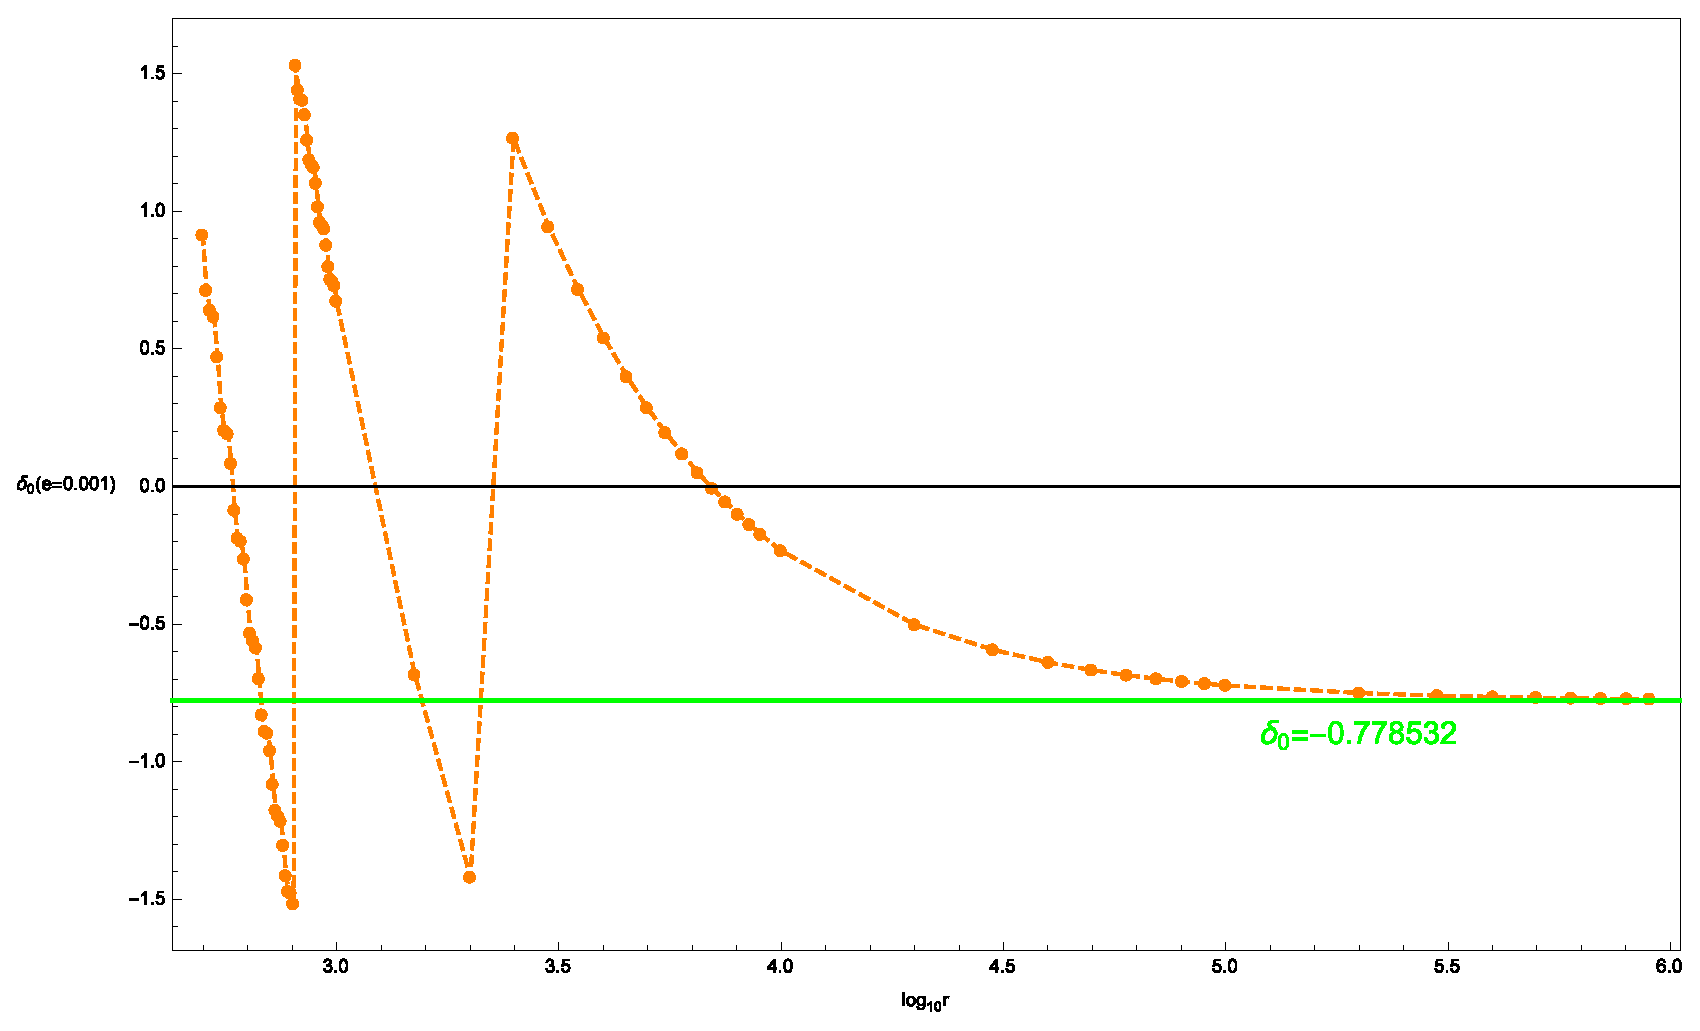
\includegraphics[width=6.2in]{Test_PhaseShift_NA_Coulomb_bothphasealter.eps}
  \caption{不同$r$下库伦势的S波相移}\label{sps1}
\end{figure}
\begin{figure}[!htbp]
  \centering
  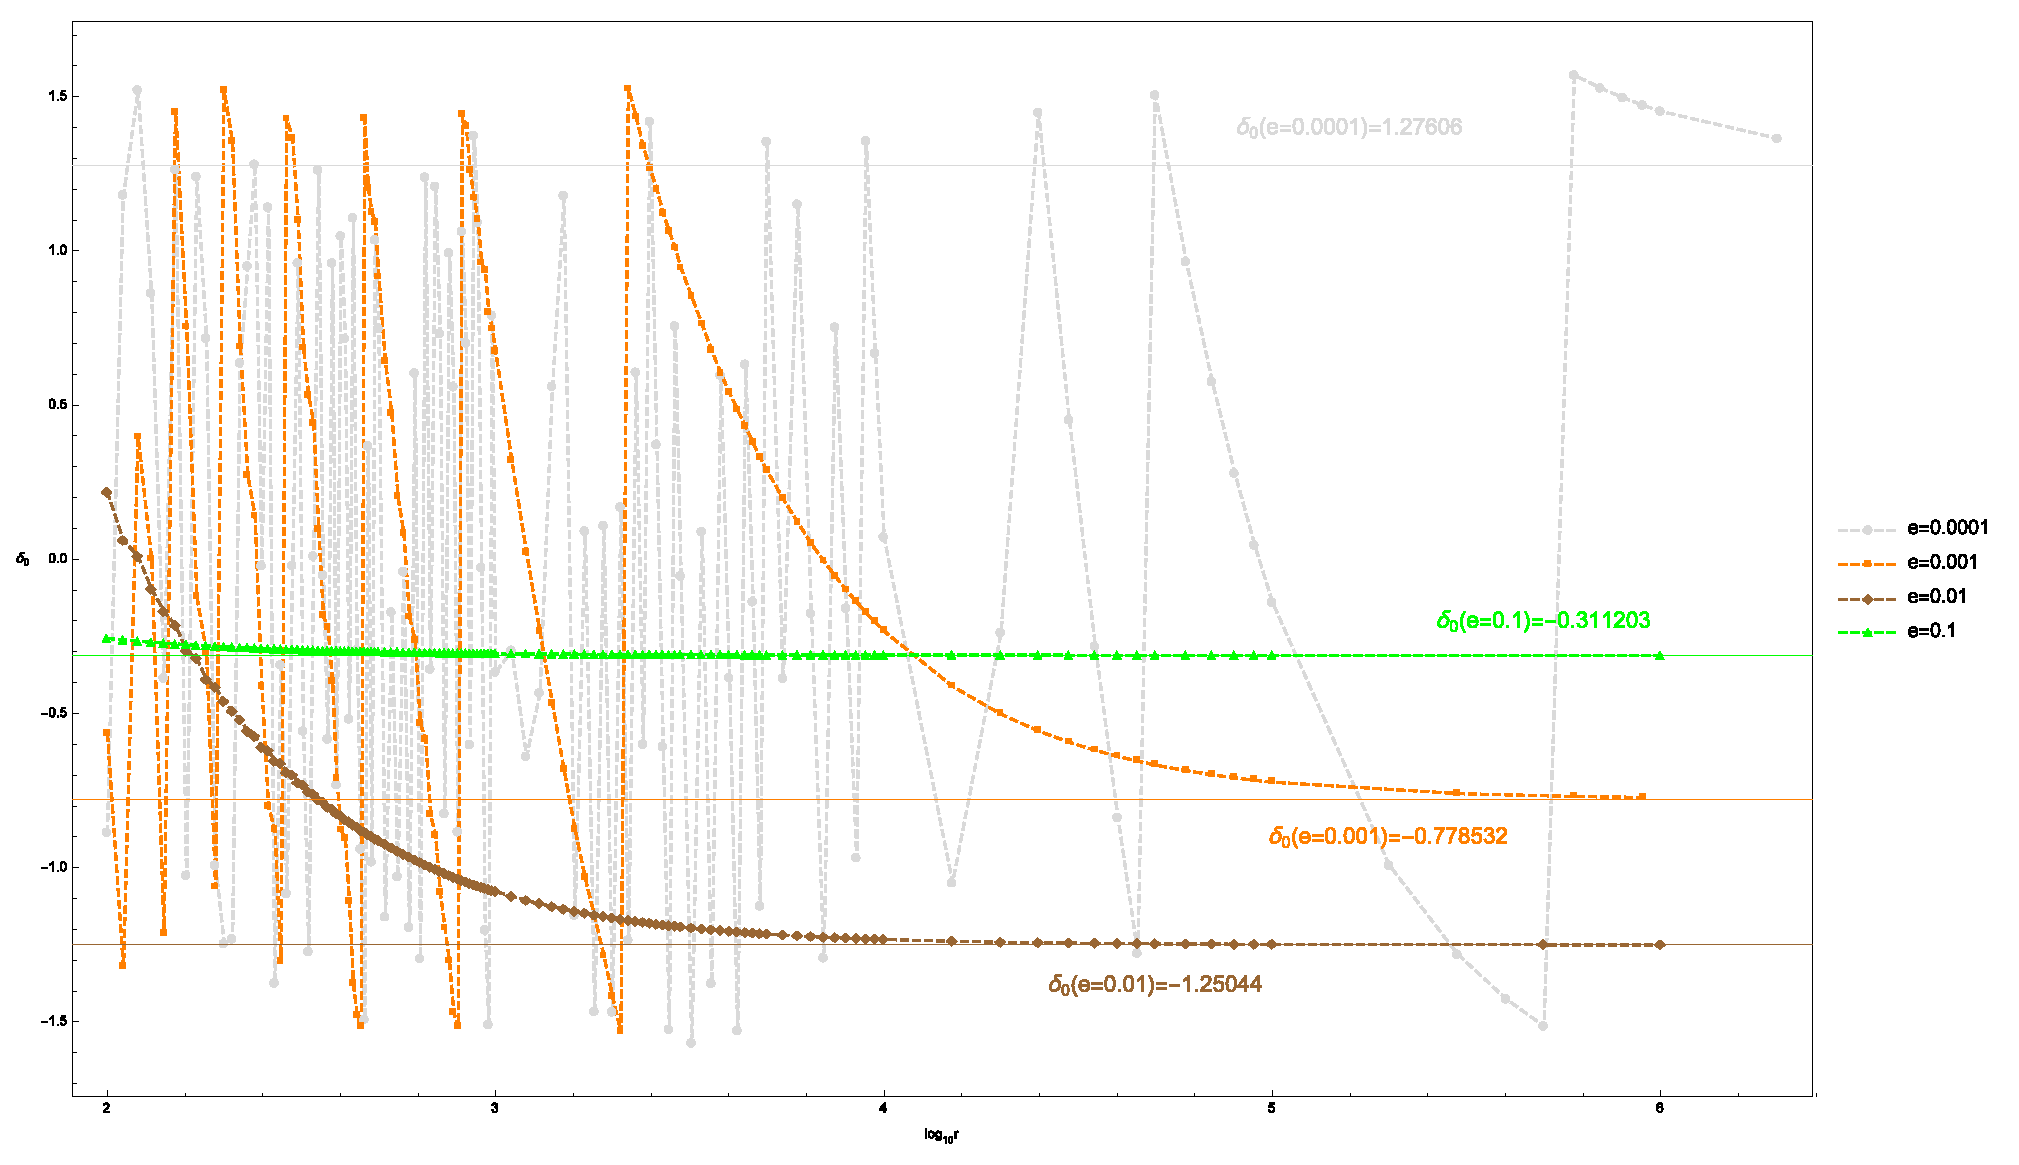
\includegraphics[width=6.2in]{Test_PhaseShift_NA_Coulomb_etest.eps}
  \caption{不同$e$下库伦势的S波相移与其解析解的比较}\label{sps3}
\end{figure}
%\subsubsection{真实势(汤川势拟合)}
%同上,利用\eqref{Coulombinffrac2},对S波相移进行求解。在$r=50$附近,$\delta_0(e=0.001)$与Lepage所给出的值较接近,但是更高能量的(如$\delta_0(e=0.1)$则在$r\in[20,200]$之间均不相符。
%
%是否有可能拟合的真实势与Lepage所用的真实势的差距导致在$r=50$处其相移的误差很大(尤其对于低能量的态来说)?库伦势解析解与Lepage相移值($r=50$)如下表:
%\begin{table}[!htbp]
%  \centering
%  \begin{tabular}{|cccc|}
%    \hline
%    % after \\: \hline or \cline{col1-col2} \cline{col3-col4} ...
%    e & 库伦势解析解 & Lepage相移值($r=50$) & 二者之差 \\
%    \hline
%    0.01 & -1.25044 & -0.654835316 & 0.595607 \\
%    0.03 & 0.716281 & 1.232867297 & 0.516587 \\
%    0.07 & -0.708782 & -0.57961962 & 0.129162 \\
%    0.1 & -0.311203 & -1.156444634 & -0.845242 \\
%    0.3 & 0.242033 & -0.106466466 & -0.348499 \\
%    0.7 & 0.306557 & -1.457426179 & 1.37761 \\
%    1 & 0.293923 & 1.160634967 & 0.866712 \\
%    \hline
%  \end{tabular}
%  \caption{库伦势解析解与Lepage相移值($r=50$)的比较}
%\end{table}
%
%高能量的几个相移计算值与Lepage所给出的相移的比较如下图(除$\delta_0(e=1)$以及$\delta_0(e=0.7)$外,其它相移与Lepage所给的值均有较大差距):
%\begin{figure}[!htbp]
%  \centering
%  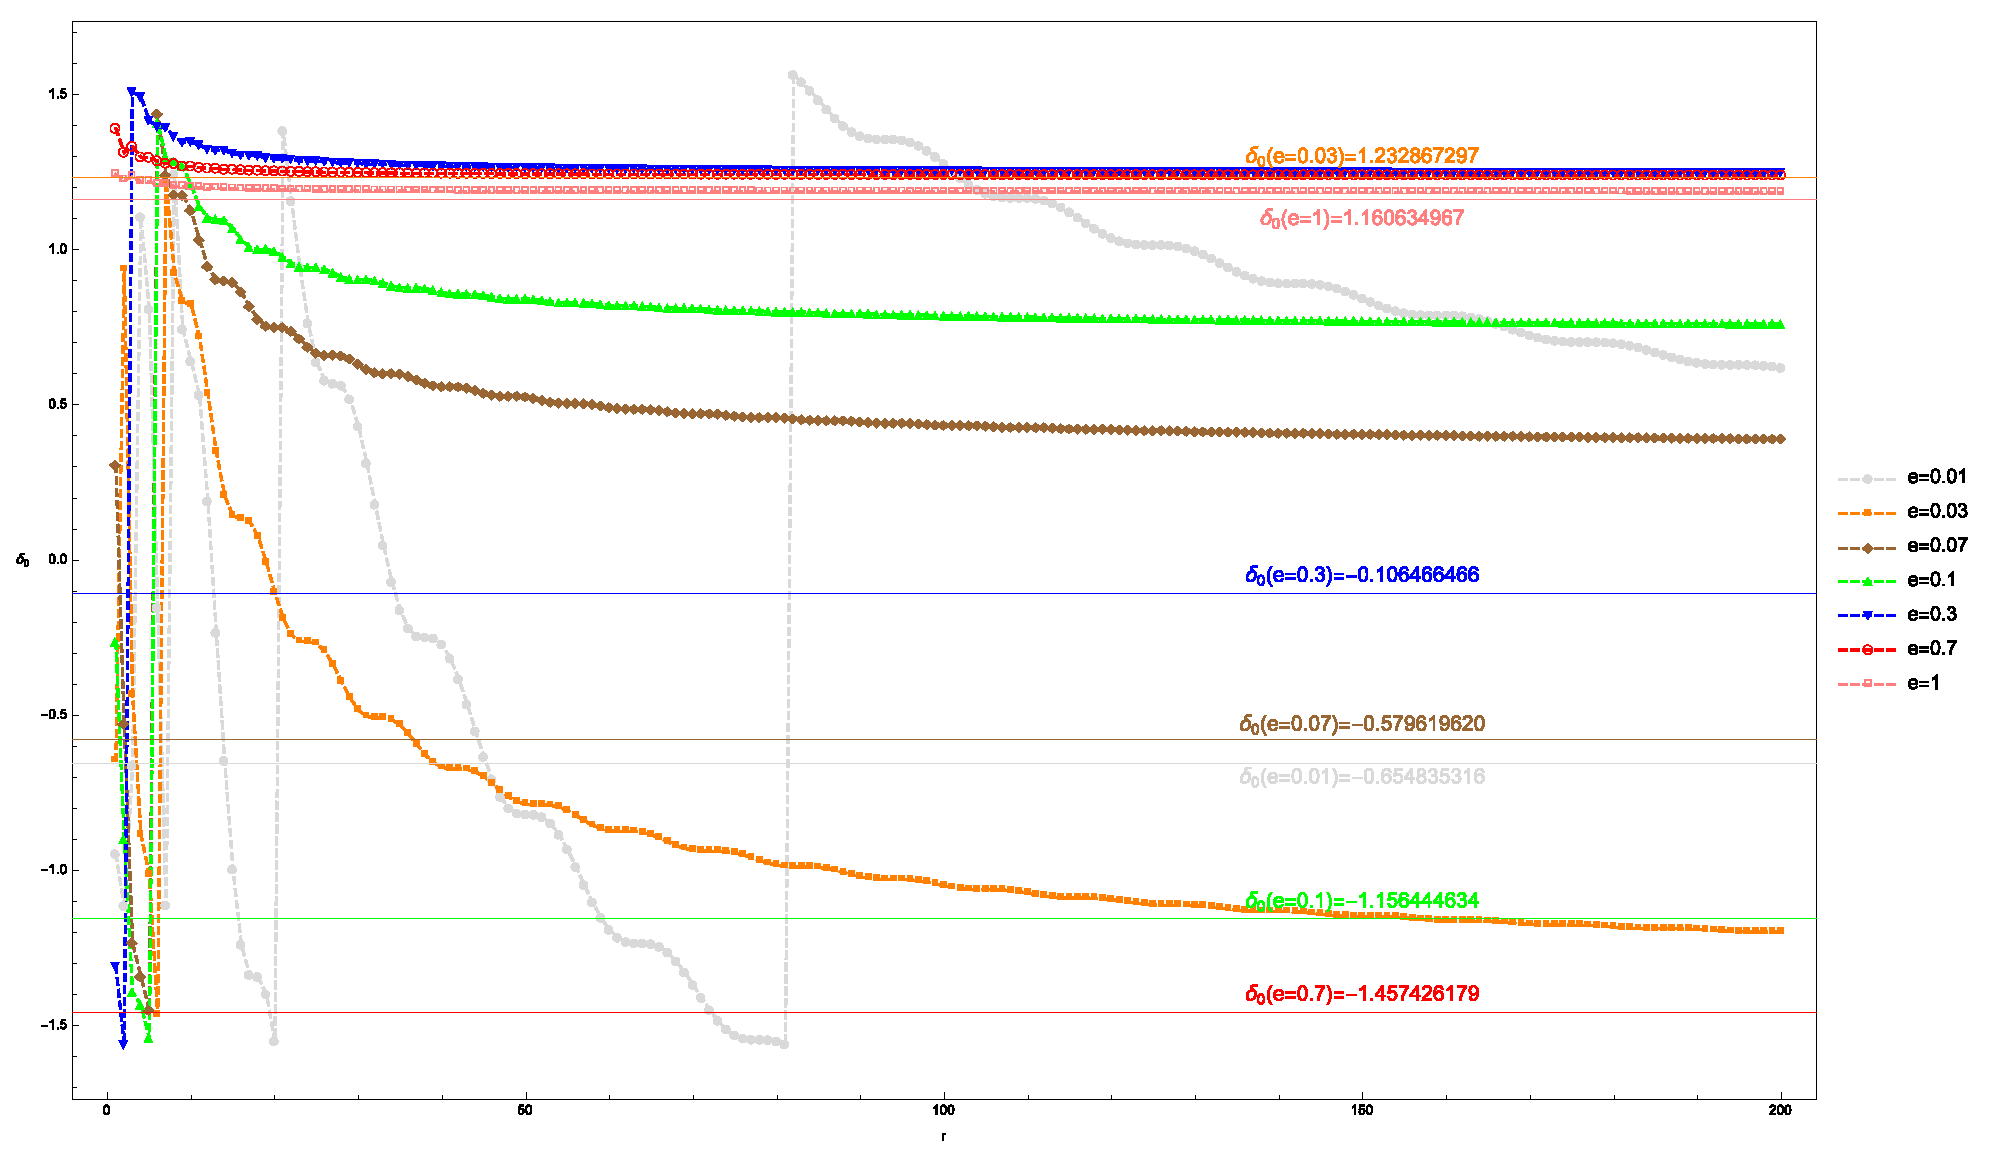
\includegraphics[width=6.2in]{Test_PhaseShift_NA_Yukawa_1.eps}
%  \caption{不同$e$下真实势(汤川势拟合)的S波相移与Lepage值的比较}\label{sps4}
%\end{figure}
%\clearpage
%\begin{figure}[!htbp]
%  \centering
%  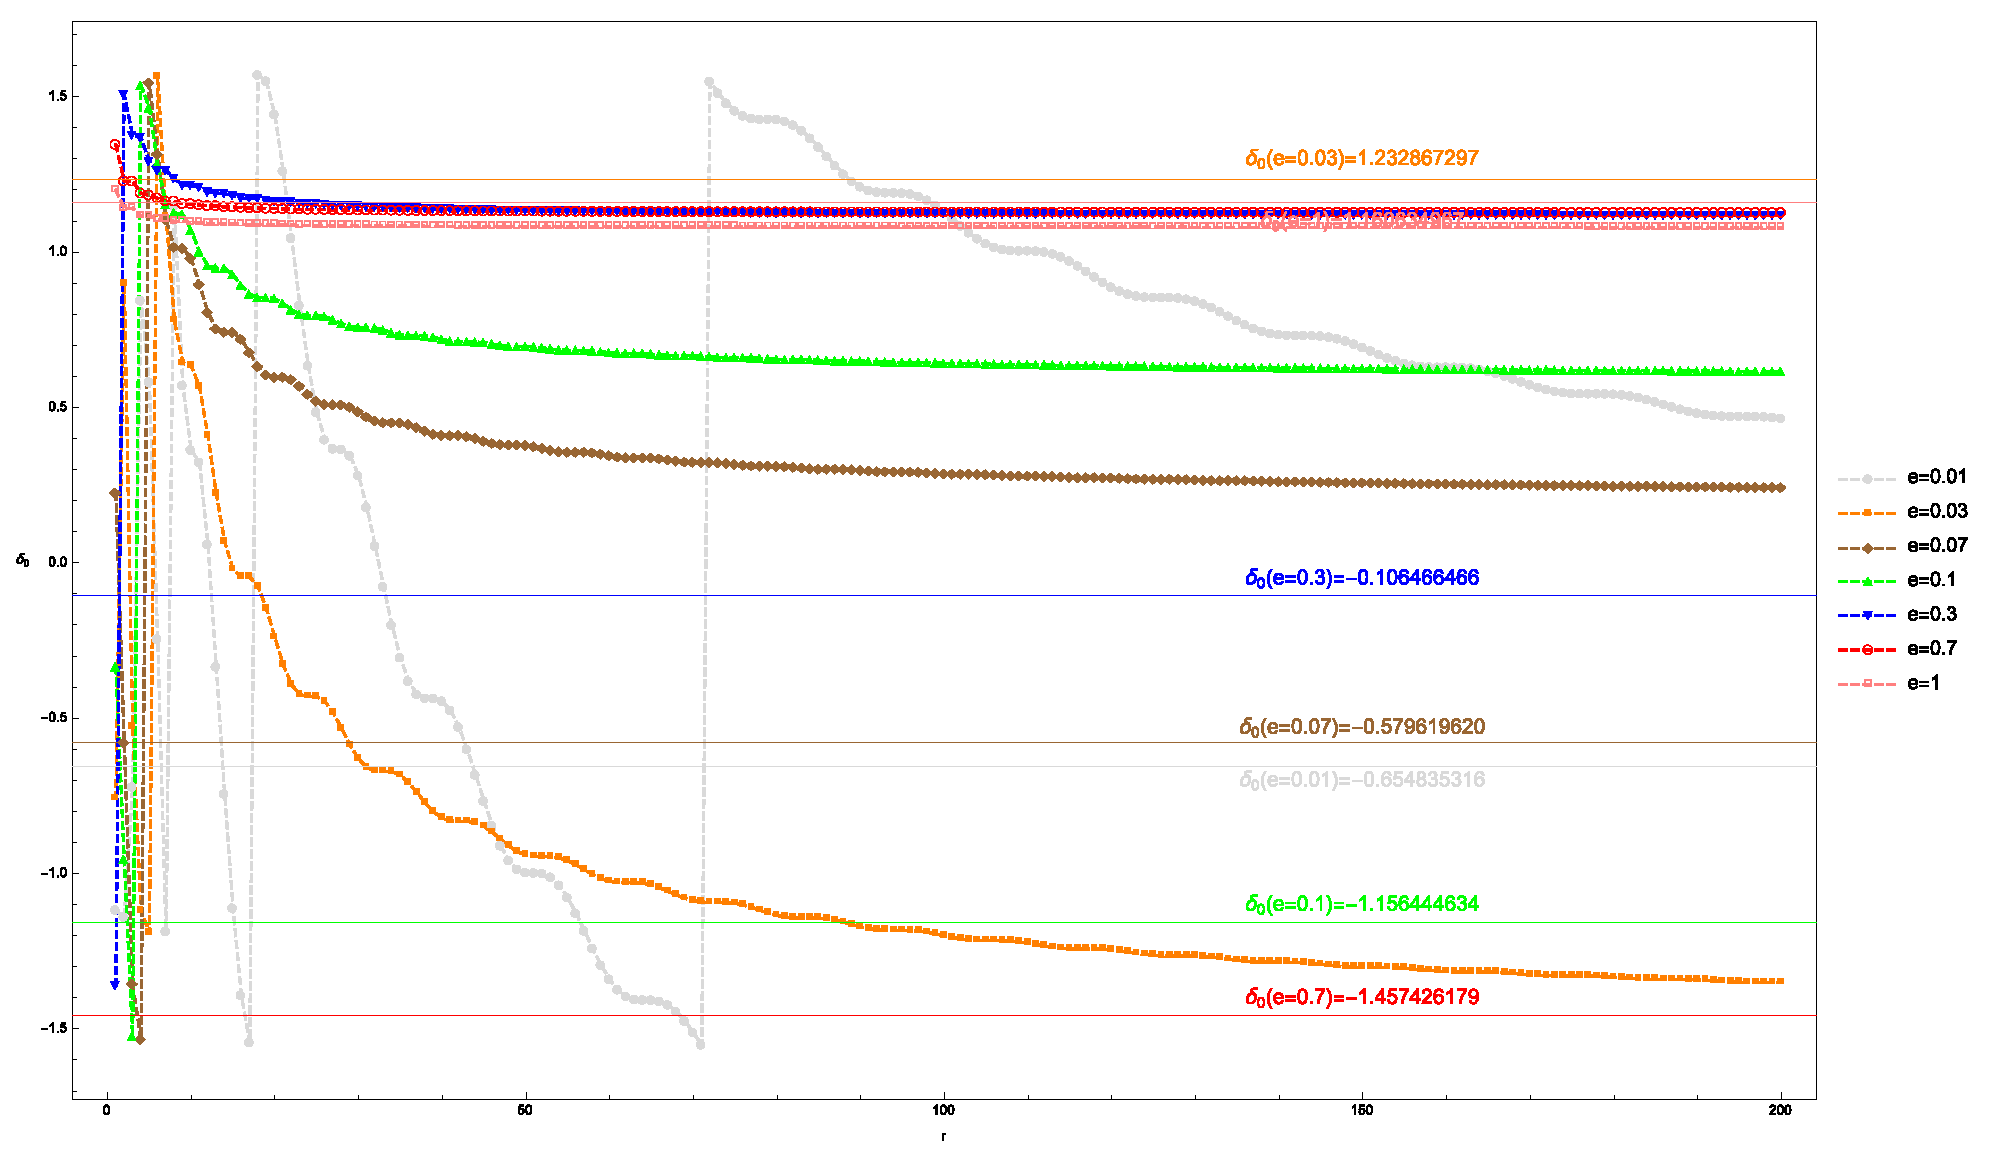
\includegraphics[width=6.2in]{Test_PhaseShift_NA_Gauss.eps}
%  \caption{不同$e$下真实势(高斯势/r拟合)的S波相移与Lepage值的比较}\label{sps5}
%\end{figure}
%\begin{figure}[!htbp]
%  \centering
%  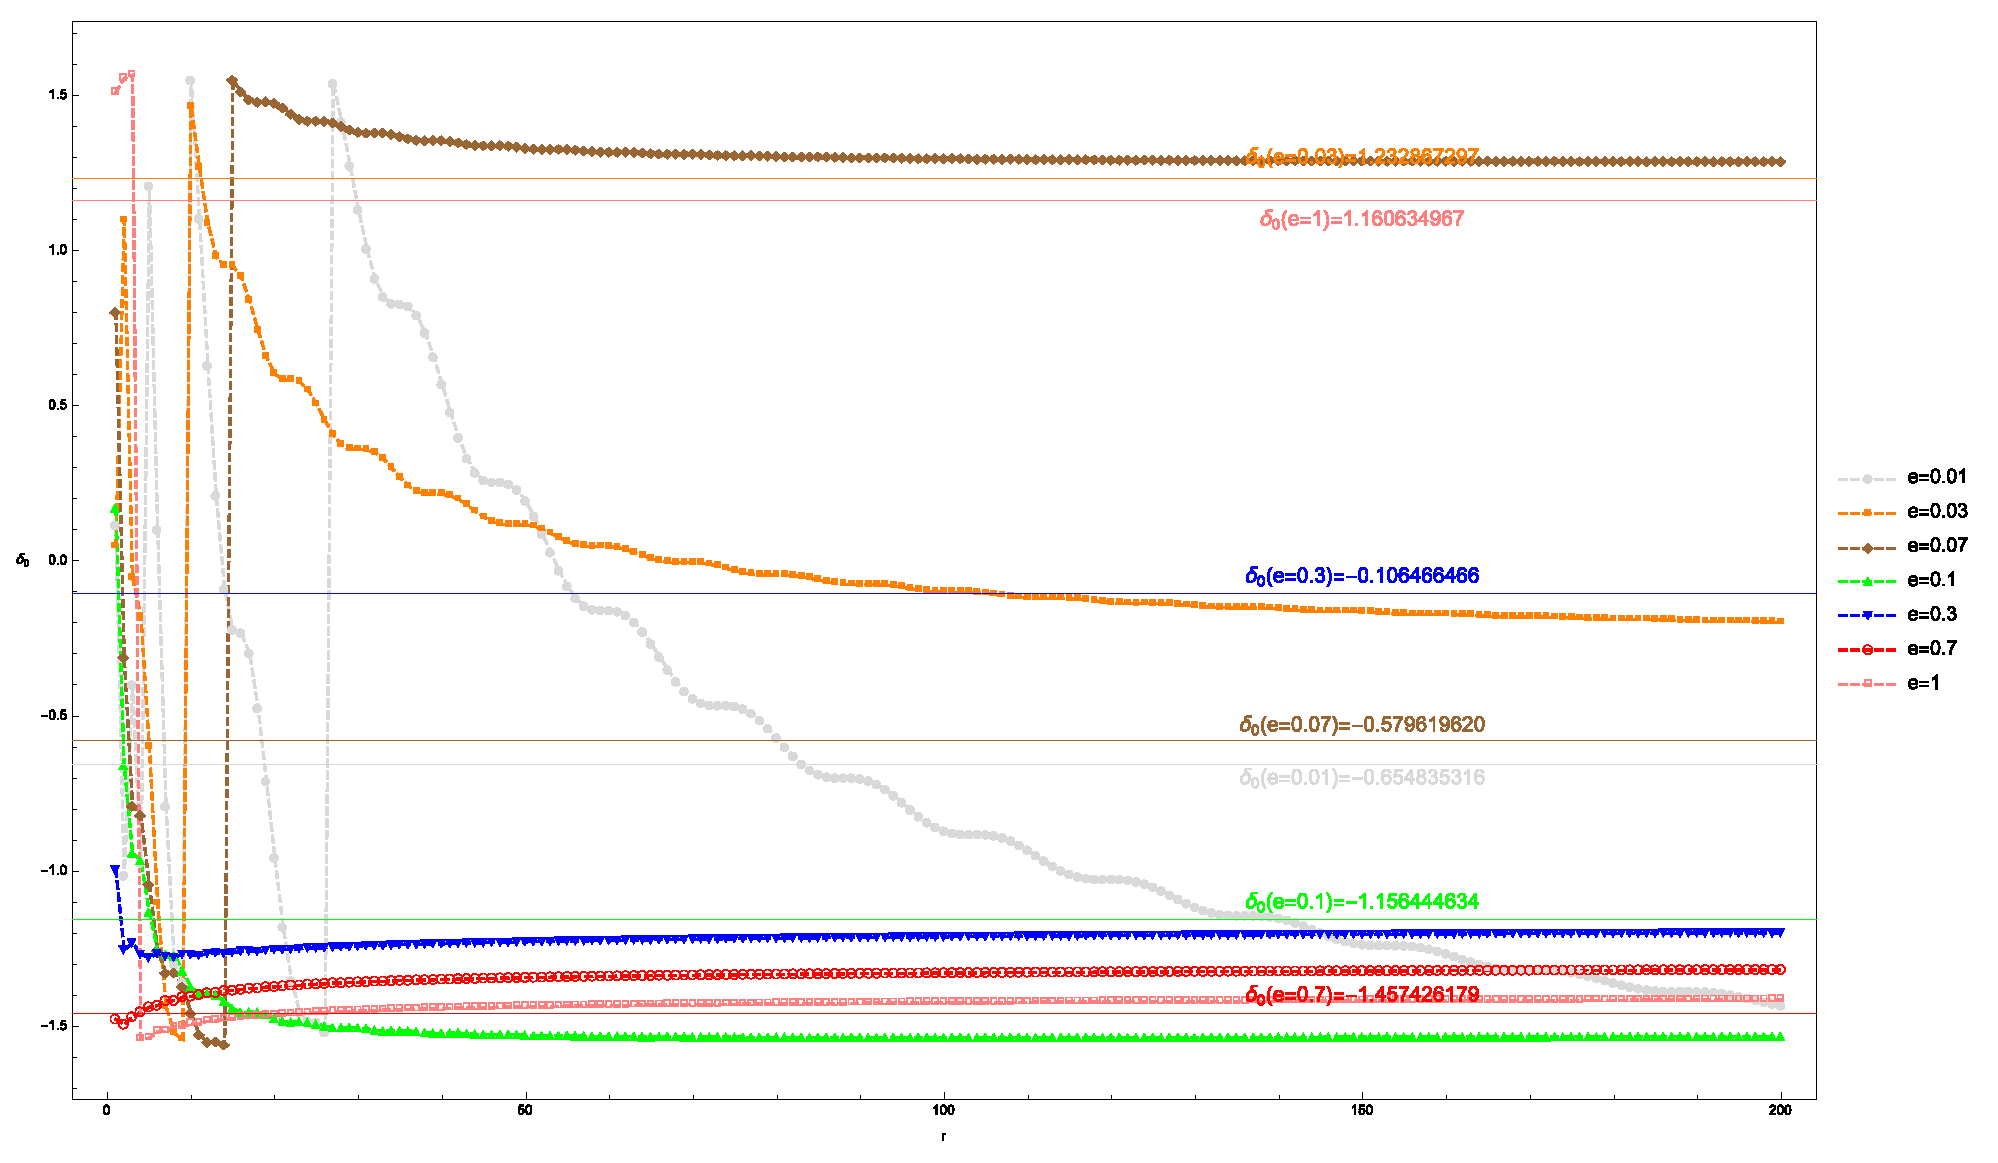
\includegraphics[width=6.2in]{Test_PhaseShift_NA_ar^b.eps}
%  \caption{不同$e$下真实势($\displaystyle\frac{a}{r^b}$拟合)的S 波相移与Lepage值的比较}\label{sps6}
%\end{figure}
%
%Lepage在库伦势基础上所附加的未知短程势对相移的影响大约在$0.5$左右。而我所拟合的真实势与未知短程势的差别是否足够大到哪怕在$e=0.7$其相移也相差甚远?又或对于不同的长程势,其渐进行为也有差别,是以不能套用相同的条件求解相移?对于前者,我对基于高斯势等其它拟合重新进行了以上计算,得到图\ref{sps5}、\ref{sps6}。相移确实产生了一些变化,变化范围最大可达到约$\pm1$内,趋势基本相同。是以不同势的差别导致相移的较大差别是可能的。而对于后者,目前讨论的所有势都是基于库伦势的,长程的行为也应当以库伦势为主,但是其渐近行为是否会有变化呢?
\subsubsection{不附加对数项}
应用条件
\begin{equation}\label{pscondition}
  \frac{u'_l(r)}{u_l(r)}=k\cot(kr+\delta_0)
\end{equation}
(在$r=50$处,这一条件虽然是近似条件,但是与利用Riccati-Bessel函数的条件相比误差已极小),对于不同的势,求解$r=50$处的相移,对于能量$E$分别取$10^{-10}$、$10^{-5}$、$0.001$、$0.003$、$0.007$、$0.01$、$0.03$、$0.07$、$0.1$、$0.3$、$0.7$、 $1$,如下三幅图,
对$E=10^{-10}$,几个不同的势与Lepage的相移几乎完全相同,$E=10^{-5}$出现了小的偏离,而之后的能量相移偏离越来越大,直到超过相移周期$\pi$。观察这些势与$\displaystyle-\frac{0.793895 e^{-0.739369 r^2}}{r}-\frac{1}{r}$的相移对比,可以发现相似的规律。势的结构越相近,相移也就越接近。相比于束缚能,相移对势的差别更敏感。
\begin{figure}[!hbtp]
  \centering
  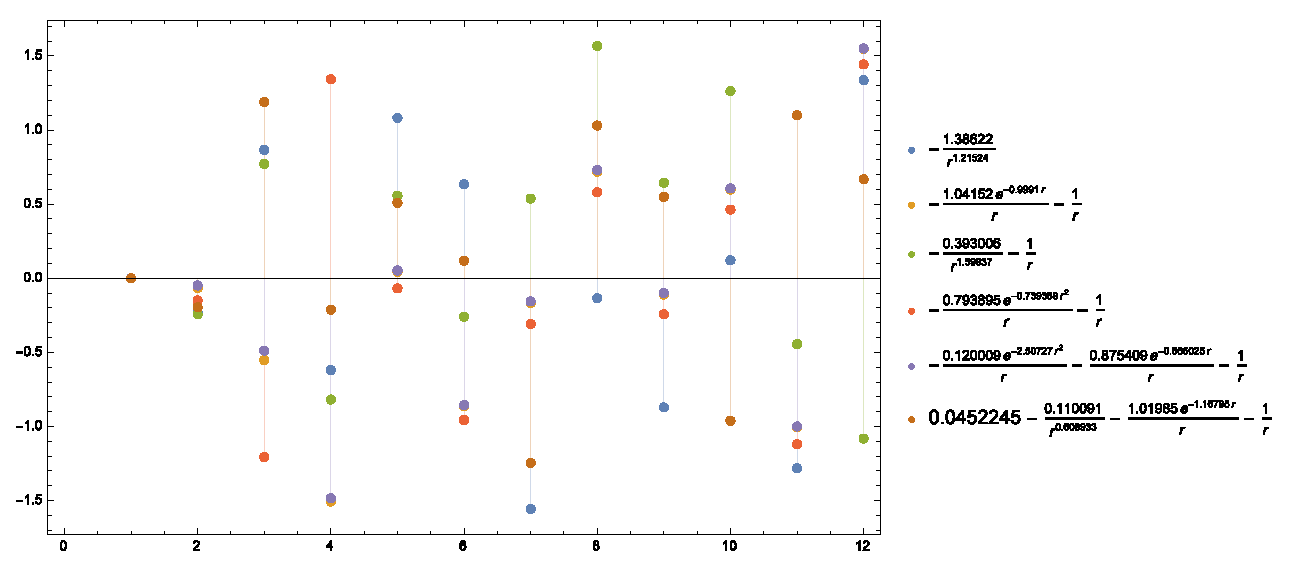
\includegraphics[width=6in]{Test_PhaseShift_delta50comparasion.eps}
  \caption{$r=50$处不同势相移值}
\end{figure}
\begin{figure}[!hbtp]
  \centering
  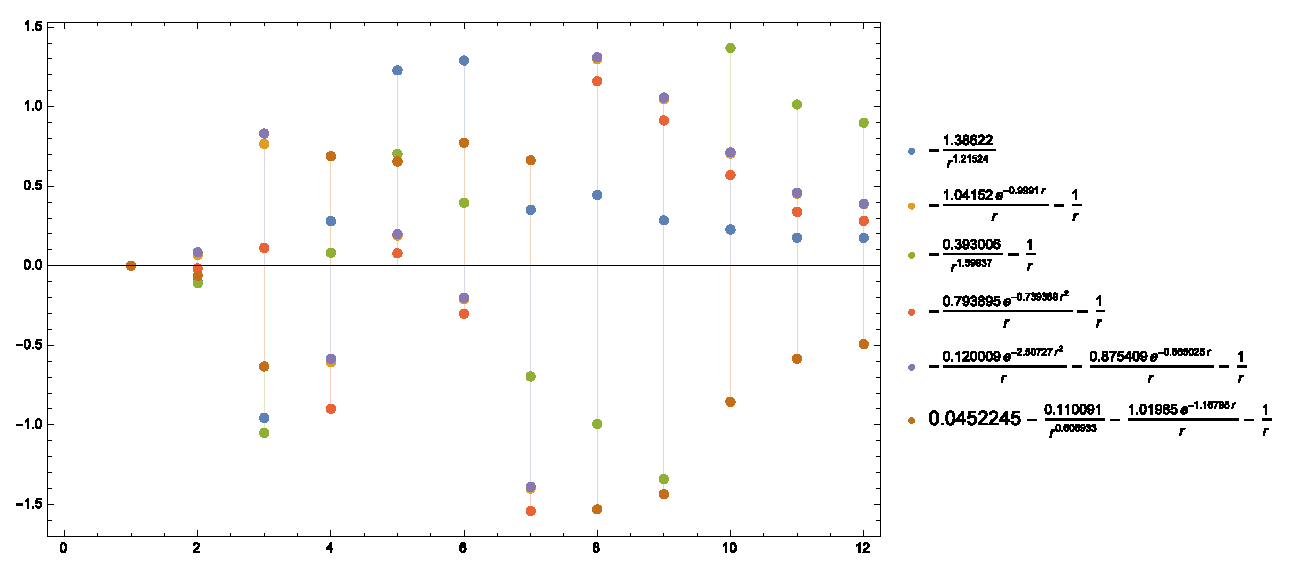
\includegraphics[width=6in]{Test_PhaseShift_delta50comparasion_2.eps}
  \caption{$r=50$处不同势相移值与Lepage相移值之差}
\end{figure}
\begin{figure}[!hbtp]
  \centering
  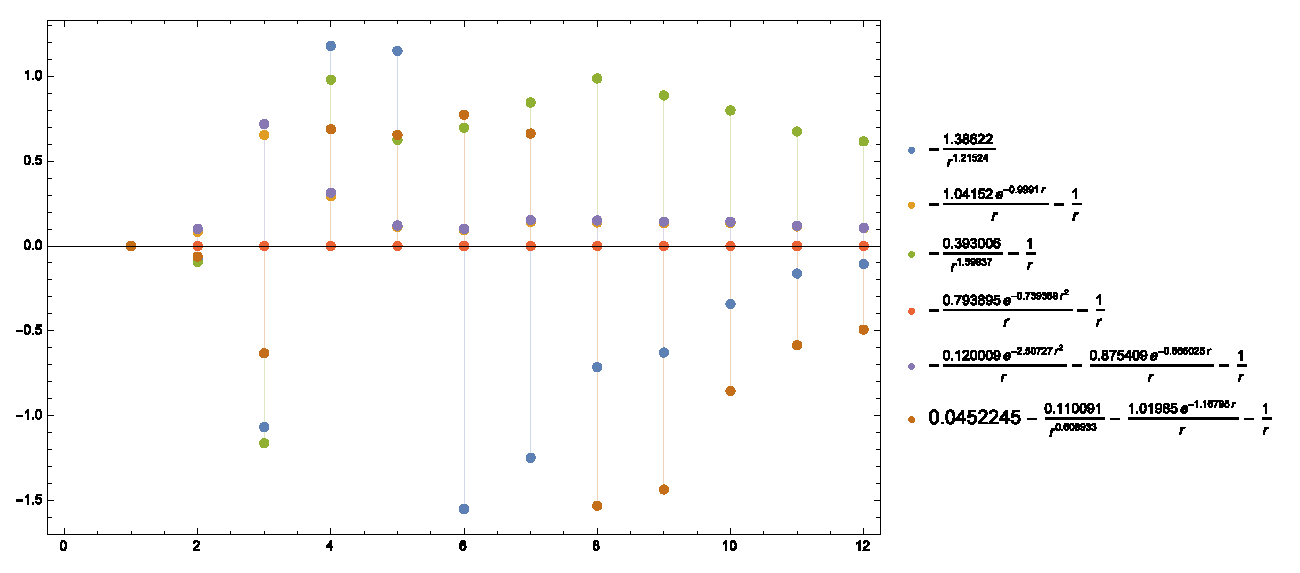
\includegraphics[width=6in]{Test_PhaseShift_delta50comparasion_3.eps}
  \caption{$r=50$处不同势相移值与$\displaystyle-\frac{0.793895 e^{-0.739369 r^2}}{r}-\frac{1}{r}$相移值之差}
\end{figure}
\clearpage
\subsubsection{有无$V_s$相减}
设:
\begin{eqnarray}
% \nonumber % Remove numbering (before each equation)
  V_0 &=& -\frac{1}{r} \\
  V_s &=& -\frac{1.04152e^{-0.9991r}}{r}
\end{eqnarray}
将$\delta_0(V_0+V_s)$与$\delta_0(V_0)$相减,则应能消去$\delta_0(V=V_0+V_s)$的库伦发散。得到减后的相移如下:
\begin{figure}[!htpb]
  \centering
  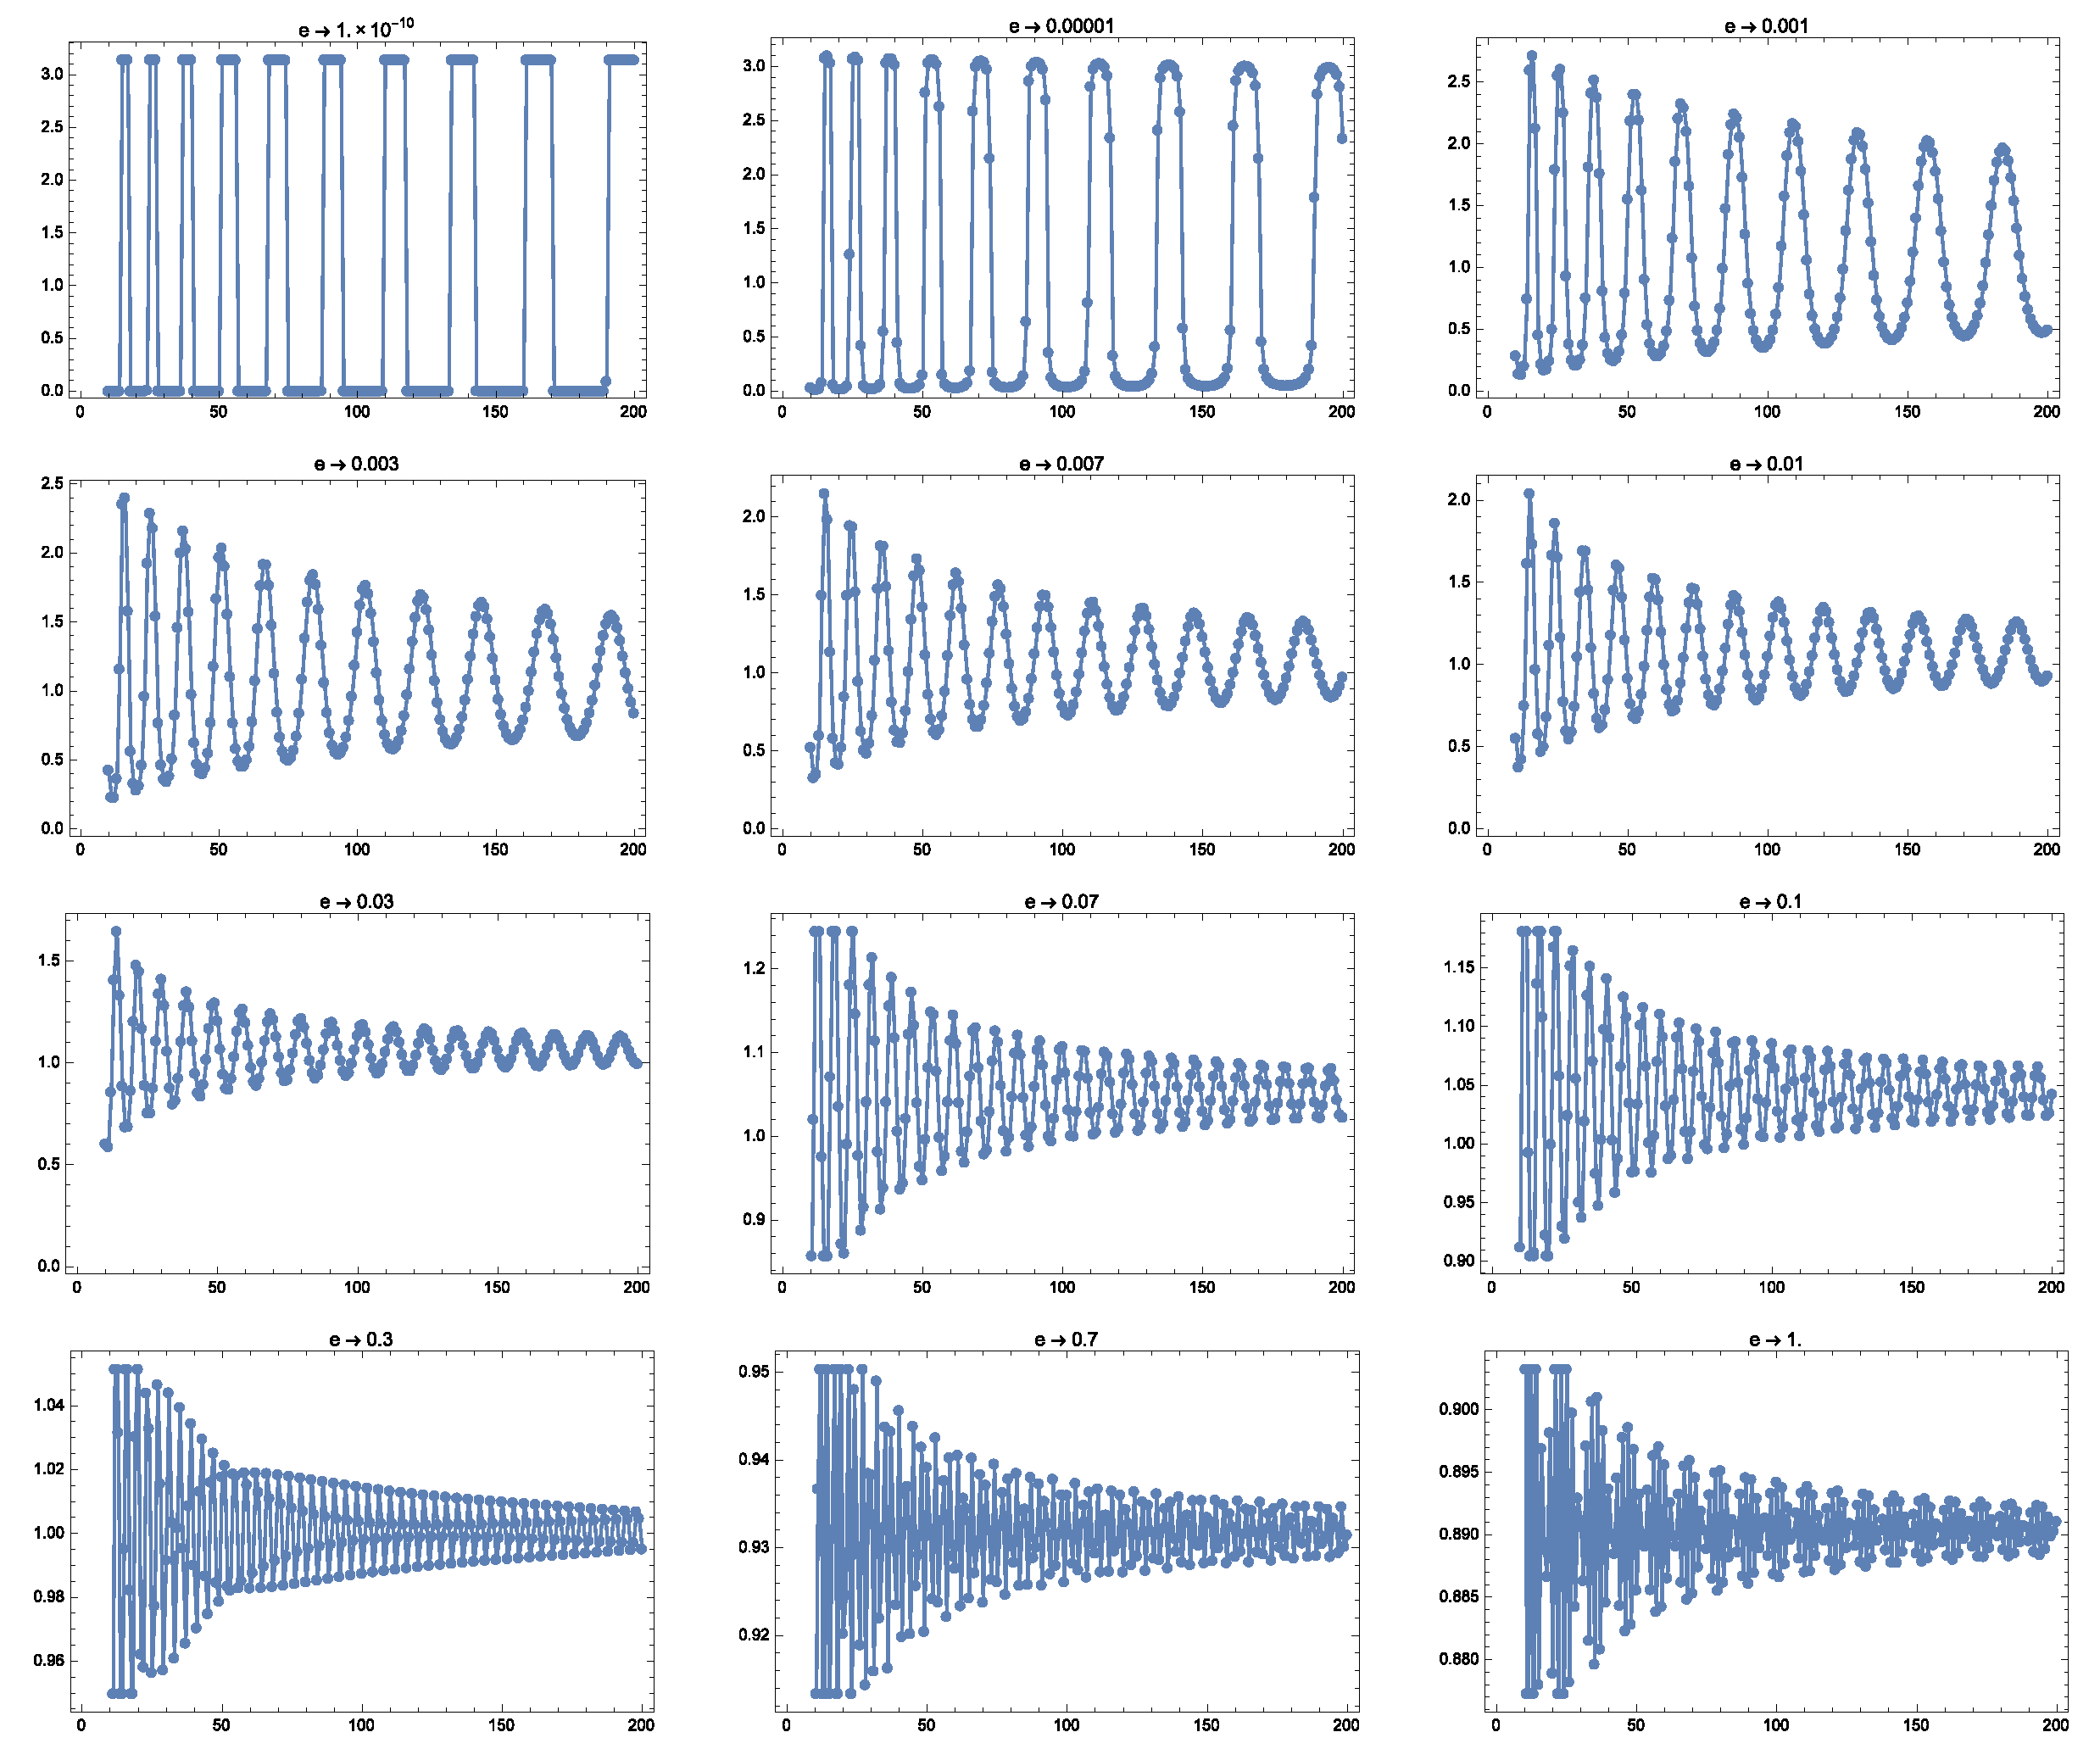
\includegraphics[width=6.2in]{Test_PhaseShift_minus.eps}
  \caption{$\delta_0(V_0+V_s)$与$\delta_0(V_0)$之差}
\end{figure}
\clearpage
\begin{figure}[!htpb]
  \centering
  \includegraphics[width=6.2in]{Test_PhaseShift_minus_1.eps}
\caption{$\delta_0(V_0+V_s)$与$\delta_0(V_0)$之差(横轴坐标为$\log_{10}r$)}
\end{figure}
但从上图可以看出减后的相移仍然依赖于$r$,虽然这一依赖比起相减之前要小,而$\delta_0(V_s)$对$r$则完全没有依赖。

\subsection{积分方程求解}
求解如下积分方程:
\begin{equation}\label{Al}
  A_l(k;r)=j_l(kr)-\frac{2mik}{\hbar^2}\times\int_{0}^{\infty}j_l(kr_<)h^{(1)}_l(kr_>)V(r')A_l(k;r')r'^2\dd r'
\end{equation}
其中$r_<$($r_>$)代表$r$和$r'$中较小(较大)的一个。再将求得的$A_l(k;r)$带入到下式中:
\begin{eqnarray}
% \nonumber % Remove numbering (before each equation)
  f_l(k) &=& e^{i\delta_l}\frac{\sin \delta_l}{k} \\
   &=& -(\frac{2m}{\hbar^2})\int_{0}^{\infty}j_l(kr)A_l(k;r)V(r)r^2\dd r
\end{eqnarray}
即可求出第$l$个分波相移$\delta_l$的值。

\eqref{Al}式是一个第二类Fredholm方程,但其核(kernel function)不是非奇异的,为此我将积分下限改为$1.0\times10^{-10}$,以避过奇点。利用已有程序求解(仅有S波,即$l=0$,并设$E$(即$k$)为已知值,具体值由Lepage原文表2得到,积分上限为$r_1=50$),并代入$f_0(k)$中求解,得到$\delta_0$的值为一个复数。由于虚数部分值较小,可近似看作$0$。

以下计算几个短程势的相移。
\subsubsection{球方势阱}
势场:
\begin{equation}\label{sq}
  V(r)=
\begin{cases}
  -V_0, & \;\;\;r\leq a \\
  0, &  \;\;\;r>a
\end{cases}
\end{equation}
其解析解为:
\begin{equation}\label{s}
  \delta_0=\arctan(\frac{k \tan k_1a-k_1\tan ka}{k_1+k\tan ka \tan k_1a})
\end{equation}
其中$\displaystyle k_1=\frac{\sqrt{2m(E+V_0)}}{\hbar}$,$\displaystyle k=\frac{\sqrt{2mE}}{\hbar}$。

当$l=0$,$m=1$,$\hbar=1$,$V_0=1$时,结果如下($n=1500$):
\begin{table}[!htbp]
  \centering
  \begin{tabular}{|c|c|c|c|c|c|c|}
    \hline
    % after \\: \hline or \cline{col1-col2} \cline{col3-col4} ...
    能量$E$ &0.0000001&0.00001& 0.001 & 0.1 & 10 & 1000\\\hline
    相移$\delta_0$计算值 &-0.0396357&-0.383836& 0.493181  & -1.08913 & 1.5069 & 1.09185  \\\hline
    相移$\delta_0$理论值 &-0.0350844&-0.34843& 0.42248 & -1.08401 & 1.50878 & 1.11759  \\\hline
  \end{tabular}
  \caption{不同能量对应的相移计算值与理论值}\label{sqq}
\end{table}
\subsubsection{$\displaystyle V(r)=\frac{\alpha}{r^2}$}
势场:
\begin{equation}\label{VVV}
  V(r)=\frac{\alpha}{r^2}
\end{equation}
根据解析解,
\begin{equation}\label{}
  \delta_l=-\frac{\pi}{2}\bqty{\sqrt{(l+\frac{1}{2})^2+\frac{2 m \alpha}{\hbar^2}}-(l+\frac{1}{2})}
\end{equation}
当$l=0$,$m=1$,$\alpha=1$,$\hbar=1$时,$\displaystyle \delta_0=-\frac{\pi}{2}\approx-1.5707963$。
\begin{table}[!htbp]
  \centering
  \begin{tabular}{|c||c|c|c|c|}
    \hline
    % after \\: \hline or \cline{col1-col2} \cline{col3-col4} ...
    \backslashbox{能量}{$r_1$} & 5 & 50 & 500 & 5000\\\hline\hline
    0.0001 & -0.0353524 & -0.350575 & -1.43881 & -1.55665  \\\hline
    0.001 & -0.11171 & -1.0149 & -1.52677 & -1.56628  \\\hline
    0.01 & -0.350575 & -1.43881 & -1.55665 & -1.56761  \\\hline
    0.1 & -1.0149 & -1.52677 & -1.56629 &   \\\hline
    1 & -1.43881 & -1.55665 & -1.5677 &   \\
    \hline
  \end{tabular}
  \caption{不同$r_1$不同能量对应的相移计算值}\label{r^2}
\end{table}\\
其结果基本与微分方程解出的一致,存在约$0.0001\%$到$2\%$的差别。
\clearpage
\section{基于Lepage文的一些计算}
根据所给的三组数据,我首先对其进行了拟合,画出Lepage文中TrueV与$a^2$、$a^4$的有效势的对照图,然后根据拟合得到的TrueV势函数求解薛定谔方程尝试得到Lepage所给出的几个S波能量本征值。关于相移,因为能量的计算还有一些问题没有解决,暂时没有着手计算。
\subsection{对三组数据的拟合}
已知有效势的形式:
\begin{eqnarray*}
% \nonumber % Remove numbering (before each equation)
  V_{eff}(\vb{r}) &=& -\frac{\alpha}{r}\;erf\pqty{\frac{r}{\sqrt{2}a}} \\
   &\phantom{=}& +c\; a^2\;\delta_a^3(\vb{r}) \\
   &\phantom{=}& +d_1\;a^4\;\laplacian{\delta_a^3(\vb{r})}+d_2\;a^4\;\div{\delta_a^3(\vb{r})}\grad \\
   &\phantom{=}& +\dots \\
   &\phantom{=}& +g\;a^{n+2}\;\nabla^n\delta_a^3(\vb{r}) \\
   &\phantom{=}& \dots\;\text{,}
\end{eqnarray*}
其中smeared delta functon定义为$\displaystyle\delta_a^3(\vb{r})=\frac{e^{-\frac{r^2}{2a^2}}}{(2\pi)^{\frac{3}{2}}\;a^3}$。

在精确到$a^2$的情况下,
\begin{equation}
  V_{eff}^{(a^2)}=-\frac{\alpha}{r}\;erf\pqty{\frac{r}{\sqrt{2}a}}+c\; a^2\;\delta_a^3(\vb{r}),
\end{equation}
精确到$a^4$的情况下,
\begin{equation}
  V_{eff}^{(a^4)}=-\frac{\alpha}{r}\;erf\pqty{\frac{r}{\sqrt{2}a}}+c\; a^2\;\delta_a^3(\vb{r})+d_1\;a^4\;\laplacian{\delta_a^3(\vb{r})}+d_2\;a^4\;\div{\delta_a^3(\vb{r})}\grad,
\end{equation}
将之分别作为model代入FindFit函数中求拟合参数,由Lepage给出的条件$a=1$得到最终结果:
\begin{eqnarray}
% \nonumber % Remove numbering (before each equation)
  V_{eff}^{(a^2)} &=& -2.74316\;e^{-\frac{r^2}{2}}-\frac{erf\pqty{\frac{r}{\sqrt{2}}}}{r} \\
  V_{eff}^{(a^4)} &=&  -2.55773\;e^{-\frac{r^2}{2}}+2.36456\pqty{-\frac{3\;e^{-\frac{r^2}{2}}}{2\sqrt{2}\;\pi^{\frac{3}{2}}}+\frac{e^{-\frac{r^2}{2}}\;r^2}{2\sqrt{2}\;\pi^{\frac{3}{2}}}}-\frac{erf\pqty{\frac{r}{\sqrt{2}}}}{r}
\end{eqnarray}
如图\ref{fit1}所示。TrueV的曲线拟合因为没有模型,留待下一节解决。
\newpage
\begin{figure}[!htp]
  \centering
  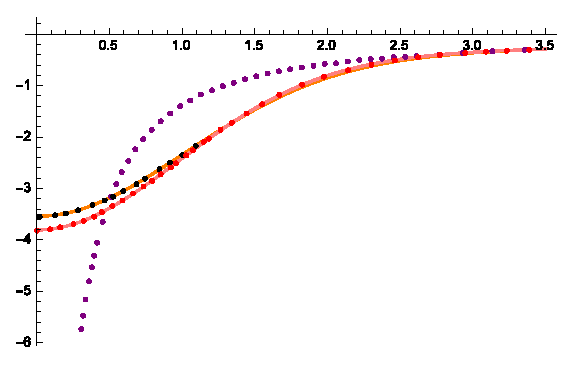
\includegraphics[width=4.50in]{Test_Veff_Three_DiracDelta&SmearedDiracDelta.eps}
  \caption{TrueV、$V_{eff}^{(a^2)}$、$V_{eff}^{(a^4)}$(原始数据点按顺序分别为紫、黑、红,后两者的拟合曲线分别为橙、粉)}\label{fit1}
\end{figure}

\subsection{重现Lepage文中的S波能量本征态}
\subsubsection{拟合TrueV}
Lepage文中并没有给出TrueV的具体解析形式。所以我使用Fit函数、FindFit函数进行其拟合函数的试探。最终发现,具备
$$
V(r)=-\frac{a}{r^b}+c\;\frac{e^{-dr}}{r}
$$
形式的拟合函数表现最好,和原始数据的差别最小。由于Lepage原文中是在一个库伦势的基础上建立的,可以作出假设$a=1$且$b=1$。最终拟合结果(对不同的model)为以下三个函数:
\begin{eqnarray}
% \nonumber % Remove numbering (before each equation)
  V_1(r) &=& -\frac{1.09835e^{-1.06921r}}{r}-\frac{1.00409}{r^{0.976102}} \\
  V_2(r) &=& -\frac{1}{r}-\frac{1.04152e^{-0.9991r}}{r} \\
  V_3(r) &=& -\frac{1.38622}{r^{1.21524}}
\end{eqnarray}
$V_2(r)$是在假设$a=1$且$b=1$下拟合出的,$V_3(r)$是以$\displaystyle-\frac{a}{r^b}$为model拟合出的。

我同时还对三个函数和原始的TrueV数据在各点上进行了对比,其函数值与原始数据的平方差(为了易于观察)如图\ref{TrueV},可以看出其中$V_1$表现与$V_2$相差无几,但是考虑到库伦势的基础,故并不采用$V_1$。$V_3(r)$在前几个点由于差距较大,超出了图的范围,并未画出。
\clearpage
\begin{figure}[!htbp]
  \centering
  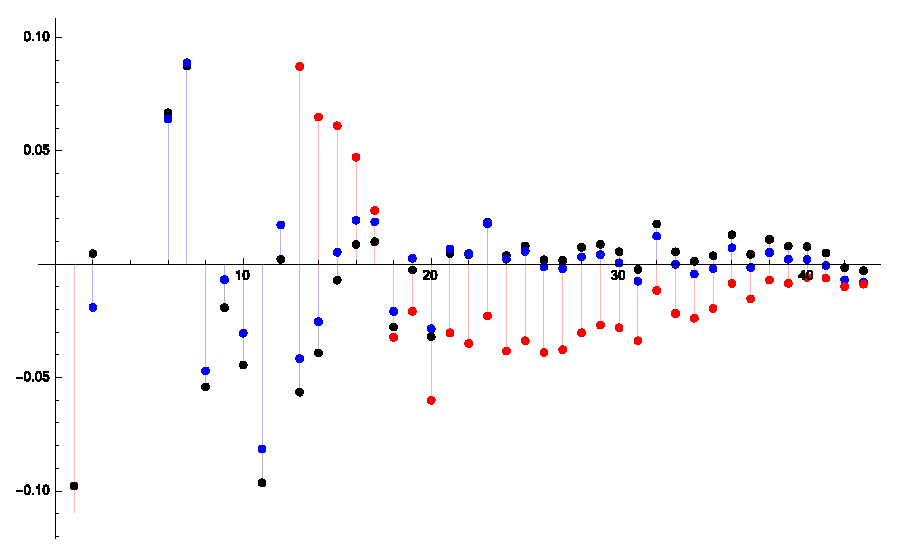
\includegraphics[width=4.5in]{Test_ReconstructLepage.eps}
  \caption{三个函数在原始数据的各点上的对比(函数值平方差,按顺序分别为蓝、黑、红)}\label{TrueV}
\end{figure}

\subsubsection{拟合的TrueV函数为$\displaystyle-\frac{1.38622}{r^{1.21524}}$}
采用$V_3(r)$为TrueV的函数,类似之前的讨论求解。结果如表\ref{V3swave}。
\begin{table}[!htbp]
  \centering
  \begin{tabular}{|cccccc|}
    \hline
    % after \\: \hline or \cline{col1-col2} \cline{col3-col4} ...
    能级 & 能量计算值 & Lepage能量值 & 能级 & 能量计算值 & Lepage 能量值 \\
    \hline
    1S & 1.31401 & 1.28711542 & 6S & 0.0168508 & 0.0155492598 \\
    2S & 0.213295 & 0.183325753  & \dots &   & \\
    3S & 0.0749002 & 0.0703755485 & 10S & 0.00536301 & 0.00534541931 \\
    4S & 0.0387671 & 0.0371495726 & 20S & 0.00126957 & 0.00129205010 \\
    5S & 0.02289 & 0.0229268241  &  &  &  \\
    \hline
  \end{tabular}
  \caption{$V_3\;\;$S波能量对比}\label{V3swave}
\end{table}
\subsubsection{拟合的TrueV函数为$\displaystyle-\frac{1}{r}-\frac{1.04152e^{-0.9991r}}{r}$}
采用$V_2(r)$为TrueV的函数,类似之前的讨论求解。结果如表\ref{V2swave}。可以看出总体误差在$1\%$左右,并且能级越高,误差越小,基态的误差最大。除了计算过程中可能的问题外,这也可能是由于$V_2(r)$与Lepage实际使用的势函数仍有不同,且在$r$较小时差别较大的原因。
\clearpage
\begin{table}[!htbp]
  \centering
  \begin{tabular}{|cccccccc|}
    \hline
    % after \\: \hline or \cline{col1-col2} \cline{col3-col4} ...
    能级 & 能量计算值 & Lepage能量值 & 相对误差 & 能级 & 能量计算值 & Lepage 能量值 & 相对误差 \\
    \hline
    1S & 1.33732 & 1.28711542 & 3.90057\% & 6S & 0.0156184 & 0.0155492598 & 0.444587\% \\
    2S & 0.186434 & 0.183325753 & 1.69544\% & \dots &   &  & \\
    3S & 0.0710575 & 0.0703755485 & 0.968963\% & 10S & 0.00535929 & 0.00534541931 & 0.259539\% \\
    4S & 0.0374072 & 0.0371495726 & 0.693401\% & 20S & 0.0012937 & 0.00129205010 &0.127336\%\\
    5S & 0.023051 & 0.0229268241 & 0.541494\% &  &  & & \\
    \hline
  \end{tabular}
  \caption{$V_2\;\;$S波能量对比}\label{V2swave}
\end{table}
\subsection{对TrueV的其他几个拟合}
目前我所用的是汤川势,类似于下文尝试的高斯势,指数衰减势有同样的问题,与原始数据的吻合度较低。故在最初Fit真实势的时候我在粗略测试了指数衰减势之后就将其除以$r$,变成汤川势的形式,吻合度大大上升。

\begin{figure}[!htbp]
  \centering
  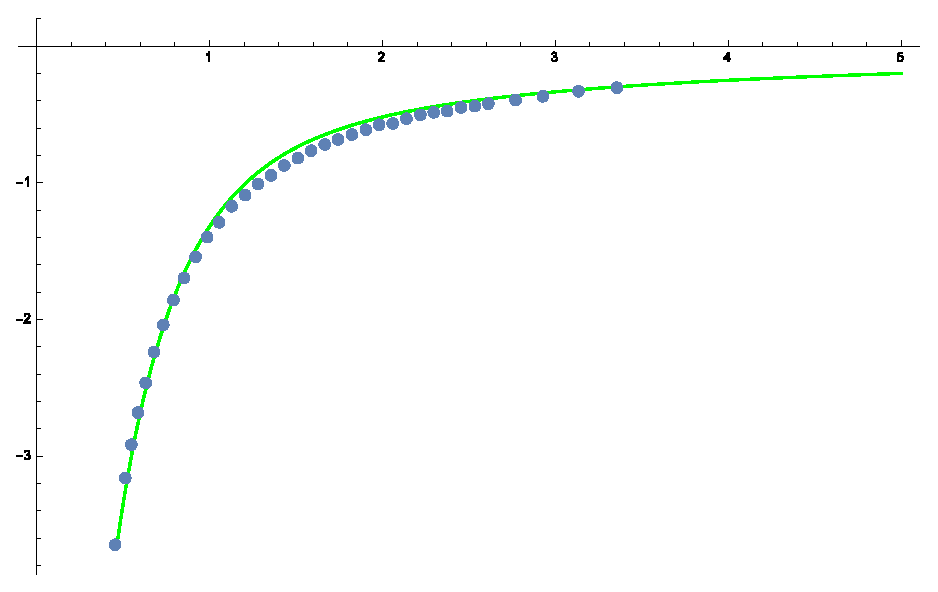
\includegraphics[width=5.2in]{Test_ReconstructLepage3.eps}
  \caption{指数衰减势函数图像}
\end{figure}
\clearpage
\begin{figure}[!htbp]
  \centering
  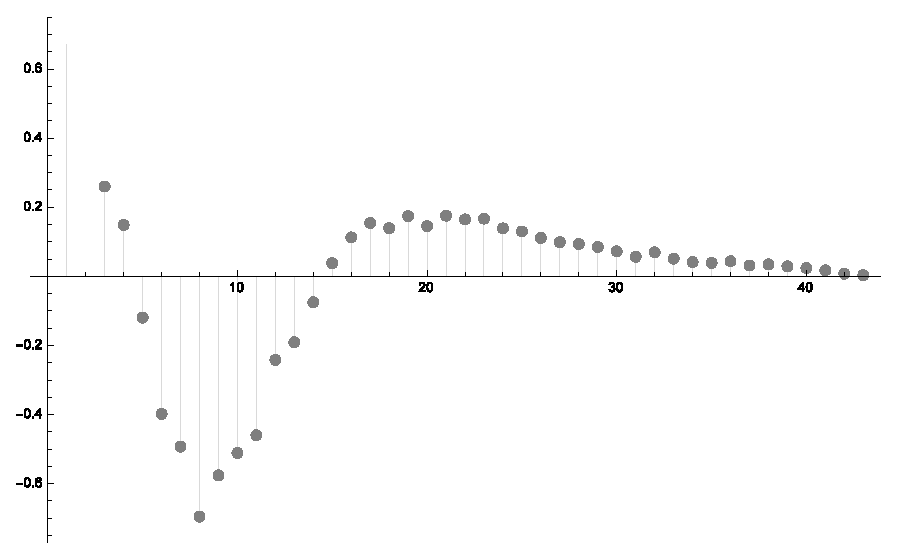
\includegraphics[width=5.2in]{Test_ReconstructLepage1.eps}
  \caption{指数衰减势在原始数据的各点上的对比(函数值平方差)}
\end{figure}
\subsubsection{高斯势}
势函数Fit如下:
\begin{equation}
  V_{Gauss}(r)=-2.87982 e^{-2.75997 r^2}-\frac{1}{r}
\end{equation}
于是有如下结果:
\begin{table}[!htbp]
  \centering
  \begin{tabular}{|cccccc|}
    \hline
    % after \\: \hline or \cline{col1-col2} \cline{col3-col4} ...
    能级 & 能量计算值 & Lepage能量值 & 能级 & 能量计算值 & Lepage 能量值 \\
    \hline
    1S & 1.07943 & 1.28711542 & 6S & 0.0150792 & 0.0155492598 \\
    2S & 0.163432 & 0.183325753  & \dots &   & \\
    3S & 0.0658655 & 0.0703755485 & 10S & 0.0052501 & 0.00534541931 \\
    4S & 0.0354216 & 0.0371495726 & 20S & 0.00128066 & 0.00129205010 \\
    5S & 0.0220872 & 0.0229268241  &  &  &  \\
    \hline
  \end{tabular}
  \caption{高斯势S波能量对比}
\end{table}\\
其结果明显不甚乐观,误差较大,尤其在基态上较汤川势更大。

\paragraph{高斯势/r}
势函数Fit如下:
\begin{equation}
  V_{Gr}(r)=-(1/r) - \frac{0.793895 e^{-0.739369 r^2}}{r}
\end{equation}
\begin{table}[!htbp]
  \centering
  \begin{tabular}{|cccccc|}
    \hline
    % after \\: \hline or \cline{col1-col2} \cline{col3-col4} ...
    能级 & 能量计算值 & Lepage能量值 & 能级 & 能量计算值 & Lepage 能量值 \\
    \hline
    1S & 1.28537 & 1.28711542 & 6S & 0.0153447 & 0.0155492598 \\
    2S & 0.172902 & 0.183325753  & \dots &   & \\
    3S & 0.0682977 & 0.0703755485 & 10S & 0.00530447 & 0.00534541931 \\
    4S & 0.03638 & 0.0371495726 & 20S & 0.00128719 & 0.00129205010 \\
    5S & 0.0225585 & 0.0229268241  &  &  &  \\
    \hline
  \end{tabular}
  \caption{高斯势/r S波能量对比}
\end{table}\\
其开始的几个能级表现较好,但之后的能级误差并没有大幅度下降,在高能级不如汤川势的表现。

附其函数图像于下页。
\paragraph{高斯势/r与汤川势的组合}
上述结果很自然引出了将高斯势/r与汤川势组合在一起的想法。Fit后所得结果如式\eqref{bind}。

\begin{figure}[!htbp]
  \centering
  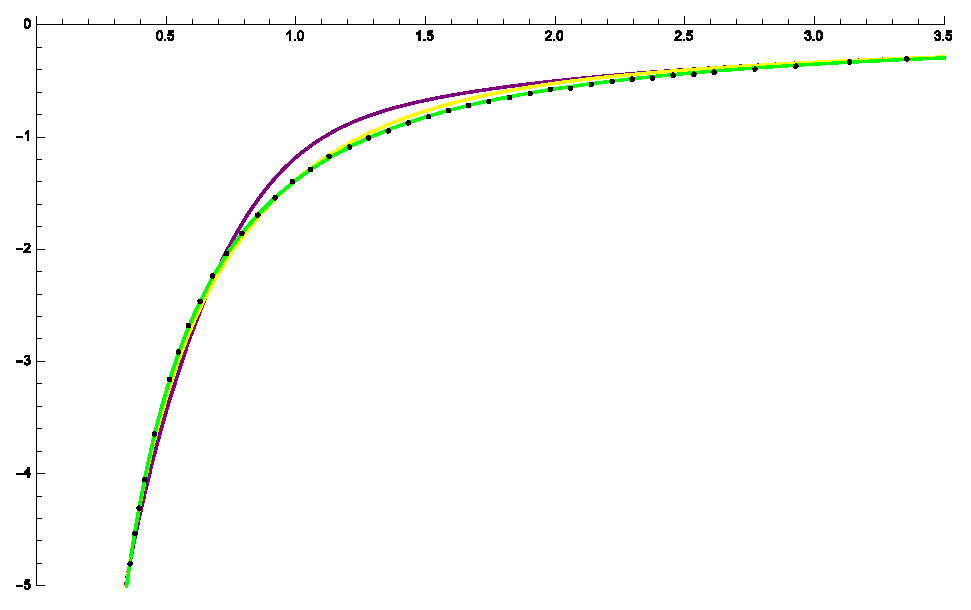
\includegraphics[width=5.2in]{Test_BindingEnergy_FitOtherwise.eps}
  \caption{汤川势与上述两势函数图像(按顺序为绿、紫、黄)}
\end{figure}

\begin{figure}[!htbp]
  \centering
  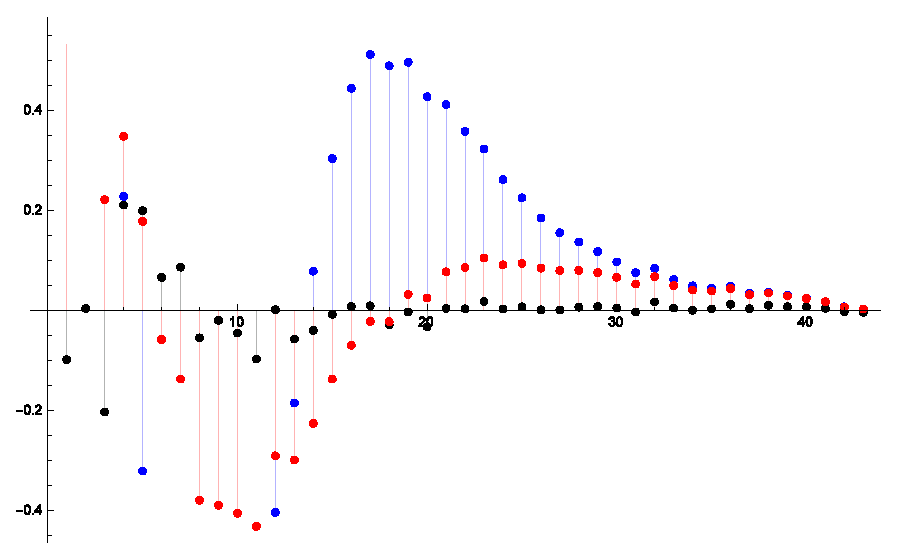
\includegraphics[width=5.2in]{Test_BindingEnergy_FitOtherwise1.eps}
  \caption{汤川势与上述两势在原始数据的各点上的对比(函数值平方差)(按顺序为黑、蓝、红)}
\end{figure}

\begin{equation}\label{bind}
  V_{bind}(x)=-\frac{0.120009 e^{-2.50727 r^2}}{r}-\frac{0.875409 e^{-0.865025 r}}{r}-\frac{1}{r}
\end{equation}
函数图像及对比见下图:
\begin{figure}[!htbp]
  \centering
  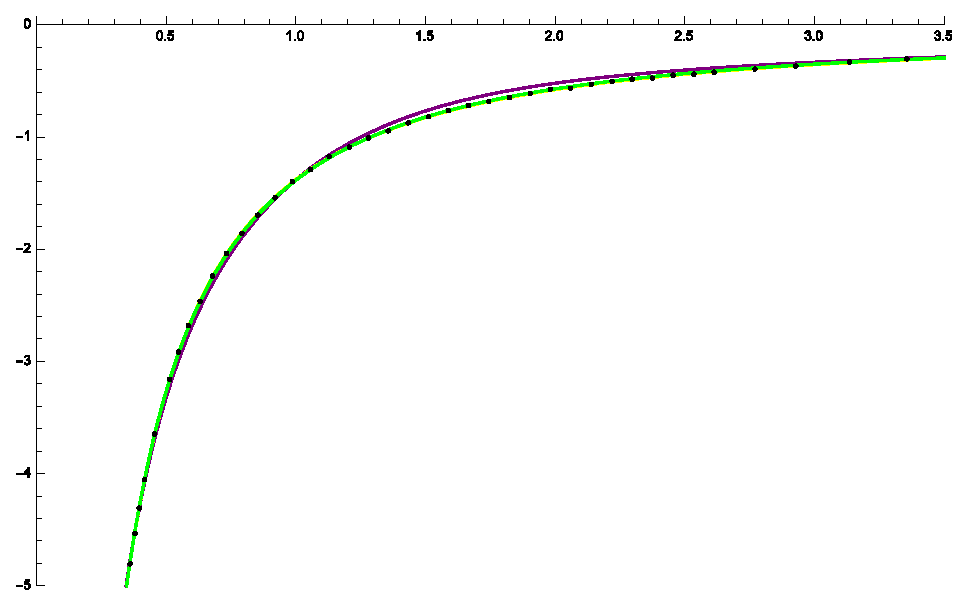
\includegraphics[width=5.2in]{Test_BindingEnergy_FitOtherwise2.eps}
  \caption{$V_{Yukawa}$、$V_{Gr}$和$V_{bind}$函数图像(按顺序为绿、紫、黄)}
\end{figure}
\clearpage
\begin{figure}[!htbp]
  \centering
  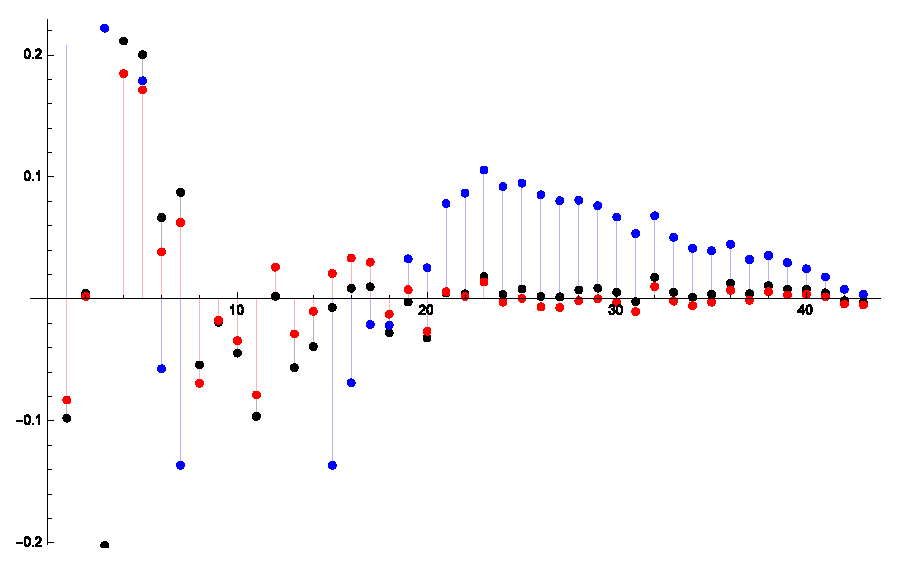
\includegraphics[width=5.2in]{Test_BindingEnergy_FitOtherwise3.eps}
  \caption{$V_{Yukawa}$、$V_{Gr}$和$V_{bind}$在原始数据的各点上的对比(函数值平方差)(按顺序为黑、蓝、红)}
\end{figure}

得到的能量本征值:
\begin{table}[!htbp]
  \centering
    \begin{tabular}{|cccccccc|}
    \hline
    % after \\: \hline or \cline{col1-col2} \cline{col3-col4} ...
    能级 & 能量计算值 & Lepage能量值 & 相对误差 & 能级 & 能量计算值 & Lepage 能量值 & 相对误差 \\
    \hline
    1S & 1.32788 & 1.28711542 & 3.16692\% & 6S & 0.0156448 & 0.0155492598 & 0.614127\% \\
    2S & 0.188546 & 0.183325753 & 2.8473\% & \dots &   &  & \\
    3S & 0.0713584 & 0.0703755485 & 1.39658\% & 10S & 0.00536445 & 0.00534541931 & 0.35602\% \\
    4S & 0.037511 & 0.0371495726 & 0.972767\% & 20S & 0.0012943 & 0.00129205010 &0.127336\%\\
    5S & 0.0230992 & 0.0229268241 & 0.751846\% &  &  & & \\
    \hline
  \end{tabular}
  \caption{组合势S波能量对比}
\end{table}\\
除了基态较汤川势稍好外,其他均不如汤川势接近。
\subsection{\emph{Figure 1}}
对于势
\begin{eqnarray}
% \nonumber % Remove numbering (before each equation)
\label{Coulomb}V_1&=&-\frac{\alpha}{r}\\
V_2&=&-\frac{\alpha}{r}+c\;\delta(\vb{r})\text{  ,}
\end{eqnarray}
其中$\alpha=1$,前者的能量容易给出:
\begin{equation}\label{e1n}
  E_{1n}=-\frac{1}{2n^2}
\end{equation}
后者能量通过一级微扰可以得到:
\begin{equation}\label{e2n}
  E_{2n}=-\frac{1}{2n^2}+c\;\frac{\delta_{l,0}}{\sqrt{\pi}\;n^3}
\end{equation}

现计算S波束缚能。

对于Lepage所给的真实束缚能,在$20S$能级处代入\eqref{e2n},可以解出$c=-.596255$;对于我之前利用我所拟合的TrueV求解的真实束缚能,同样可以解出$c=-.619584$。由此可以得到两者各能级$E_{1n}$与$E_{2n}$的值见表\ref{e2nfigure1}($E_{1n}$结果二者相同且显而易见,故不一一列出)。

\begin{table}[!htbp]
  \centering
  \begin{tabular}{|cccccc|}
    \hline
    % after \\: \hline or \cline{col1-col2} \cline{col3-col4} ...
    能级 & Lepage & 拟合TrueV & 能级 & Lepage & 拟合TrueV \\
    \hline
    1S & 1.31401 & 0.849563 & 6S & 0.0168508 & 0.0155072 \\
    2S & 0.213295 & 0.168695  & \dots &   & \\
    3S & 0.0749002 & 0.0685023 & 10S & 0.00536301 & 0.00534956 \\
    4S & 0.0387671 & 0.0367119 & 20S & 0.00126957 & 0.0012937 \\
    5S & 0.02289 & 0.0227965  &  &  &  \\
    \hline
  \end{tabular}
  \caption{按Lepage真实束缚能与拟合TrueV得到S波近似能量$E_{2n}$ 对比}\label{e2nfigure1}
\end{table}

最终得到类似Lepage原文\emph{Figure 1}的图如下:
\begin{figure}[!htbp]
  \centering
  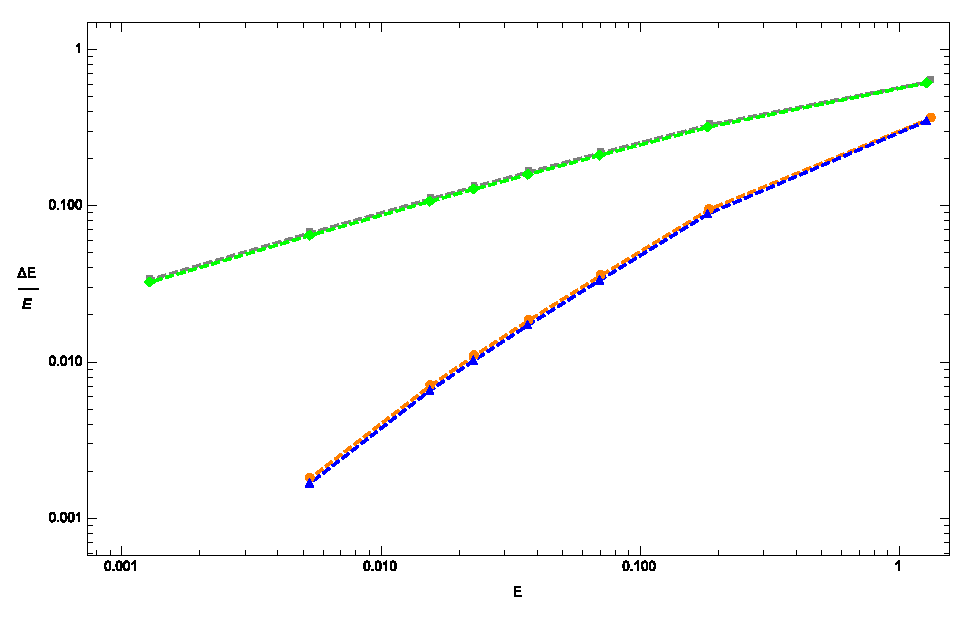
\includegraphics[width=5.2in]{Test_LepageFigure_1.eps}
  \caption{由Lepage所给能量(绿、蓝)以及拟合TrueV能量(橙、灰)得到的$E_{1n}$、$E_{2n}$ 与各自对应的真实能量的相对误差}\label{LepageFigure1}
\end{figure}
\subsection{\emph{Figure 2}}
在Lepage文中明确指出后两种使用有效理论的势是采用类似于真实势的解法得出束缚能级的,唯一的区别是用有效势代替真实势,另外在$Figure\;2$中也对此有明确的表述:“\emph{the nonperturbative effective theory}"。由此我并没有使用微扰论进行计算。

利用之前计算真实势束缚能的程序,我可以很容易得到有效势束缚能。

在精确到$a^2$的情况下,
\begin{equation}\label{Veffa2}
  V_{eff}^{(a^2)}=-\frac{\alpha}{r}\;erf\pqty{\frac{r}{\sqrt{2}a}}+c\; a^2\;\delta_a^3(\vb{r}),
\end{equation}
精确到$a^4$的情况下,
\begin{equation}\label{Veffa4}
  V_{eff}^{(a^4)}=-\frac{\alpha}{r}\;erf\pqty{\frac{r}{\sqrt{2}a}}+c\; a^2\;\delta_a^3(\vb{r})+d_1\;a^4\;\laplacian{\delta_a^3(\vb{r})}+d_2\;a^4\;\div{\delta_a^3(\vb{r})}\grad,
\end{equation}%由于有效势的系数仍需确定,这将是我所进行的第一步。
其中smeared delta functon定义为$\displaystyle\delta_a^3(\vb{r})=\frac{e^{-\frac{r^2}{2a^2}}}{(2\pi)^{\frac{3}{2}}\;a^3}$。

精确到$a^2$的有效势系数由于需要用散射相移确定,暂时不参与计算。对于精确到$a^4$的有效势,由Lepage文中给出的值,系数$c=-3.18\times4\pi$,$d_1=-0.199\times4\pi$,$d_2=0$(对S波)。
%\subsection{有效势的系数}
\subsubsection{S波束缚能级}
与计算真实势类似,我得到了各能级束缚能如下表:
\begin{table}[!htbp]
  \centering
  \begin{tabular}{|cccccc|}
    \hline
    % after \\: \hline or \cline{col1-col2} \cline{col3-col4} ...
    能级 & 能量计算值 & Lepage能量值 & 能级 & 能量计算值 & Lepage 能量值 \\
    \hline
    1S & 1.49378 & 1.28711542 & 6S & 0.0155484 & 0.0155492598 \\
    2S & 0.182098 & 0.183325753  & \dots &   & \\
    3S & 0.0703401 & 0.0703755485 & 10S & 0.00534527 & 0.00534541931 \\
    4S & 0.0371441 & 0.0371495726 & 20S & 0.00129203 & 0.00129205010 \\
    5S & 0.022925 & 0.0229268241  &  &  &  \\
    \hline
  \end{tabular}
  \caption{$V_{eff}^{(a^4)}\;\;$S波能量对比}
\end{table}
\subsubsection{重复Lepage的相对误差图}
可能是由于Lepage文中所给的有效势系数精确程度不够的原因,我所重复的图中的有效势相对误差在高能级情况下并不如原文中一般快速下降,而是有停留在$10^-5$量级上的趋势。在加大之前束缚能计算精度的情况下,束缚能仅在第10个有效数字处发生改变,变化极小,因此不太可能是由于束缚能计算误差引起这种相对误差较高的情况。

相对误差如下图:

\begin{figure}[!htbp]
  \centering
  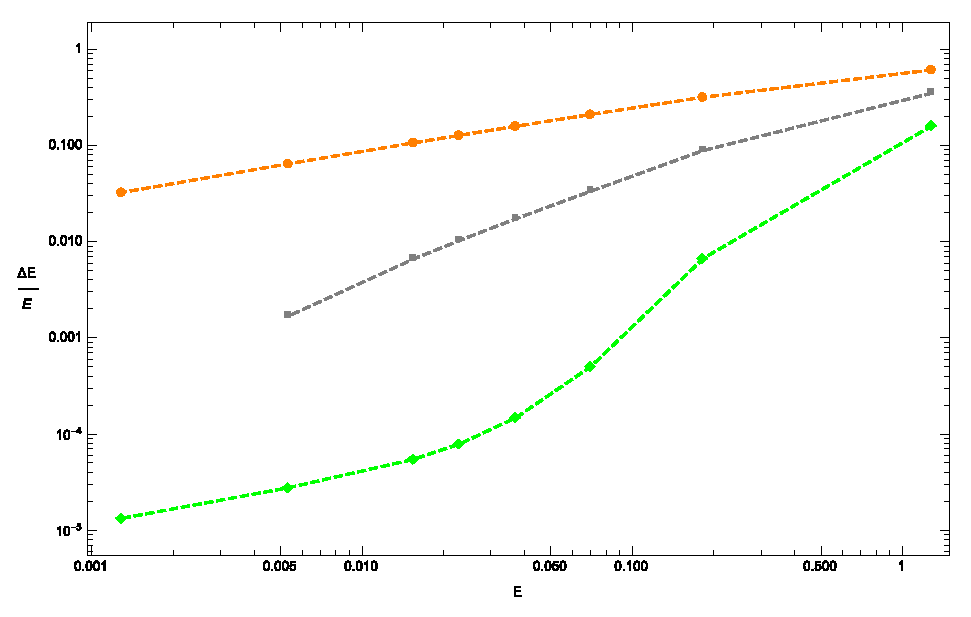
\includegraphics[width=5.2in]{Test_LepageFigure_2.eps}
  \caption{$V_1$、$V_2$、$V_{eff}^{(a^4)}$相对误差(按顺序分别为橙、灰、绿)}\label{relative error 2}
\end{figure}
由于散射相移暂时无法计算,为了验证图\ref{relative error 2}是否是由于有效势系数精度问题引起高能级数据的差别,我将系数$c$改写为$c=-(3.18+0.0008)\times4\pi$,得到下图:
\begin{figure}[!htbp]
  \centering
  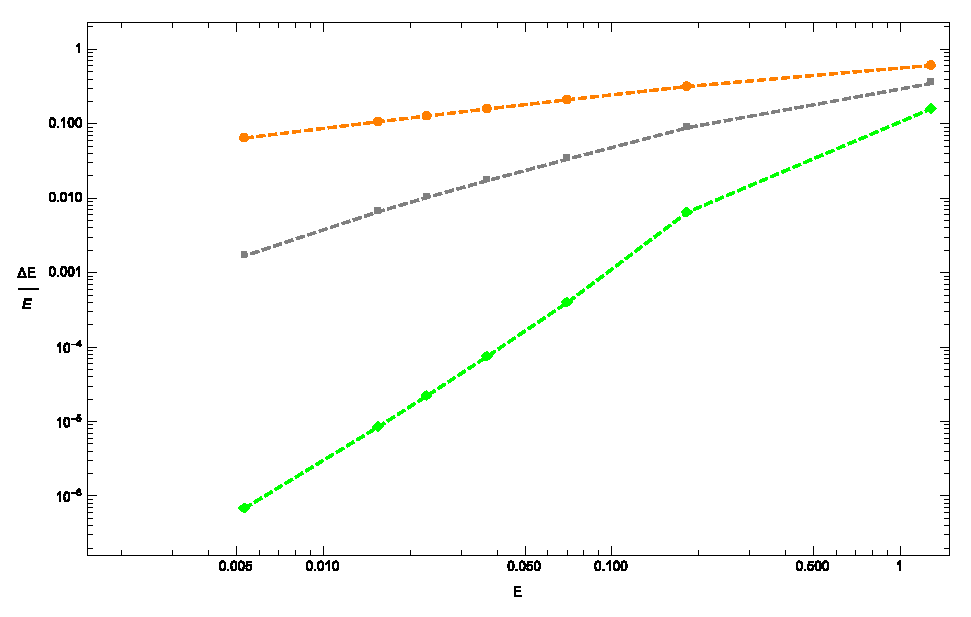
\includegraphics[width=5.2in]{Test_LepageFigure_2_2.eps}
  \caption{$V_1$、$V_2$、$V_{eff}^{(a^4)}(different\;c)$ 相对误差(按顺序分别为橙、灰、绿)}\label{relative error 2_2}
\end{figure}\\
于是可以看出图中的趋势与Lepage原图大致相同,因此可以作出猜测:数据差别的主要原因是有效势系数的精度问题。
\subsection{根据真实势(汤川势拟合)确定有效势系数}
\subsubsection{利用高能级束缚能确定系数}
现根据之前利用汤川势模型所拟合出的真实势,利用15S及20S的真实束缚能可以确定有效势\eqref{Veffa2}与\eqref{Veffa4}中的系数,除了可以假定为观测数据的真实束缚能外,无需引入其他任何条件。

于是可以得到$c^{(a^2)}=-44.291$以及$c^{(a^4)}=-40.6855$与${d_1}^{(a^4)}=2.69247$。
\subsubsection{对应束缚能及误差}
由以上确定的系数可以得到对应的束缚能及误差如下图,可以看出从总体趋势上来说,有效势的精度更高,并且确定的系数精度处在同样的数量级时,$\mathcal{O}(a^n)$幂次数越高,有效势精度越高。但是相对的,$\mathcal{O}(a^n)$幂次数越高,系数就越难精确确定(待确定的系数就越多)。第二幅图中低能量处$V_{eff}^{(a^4)}$对应相对误差所出现的抖动就是这一原因引起的。
\begin{figure}[!htbp]
  \centering
  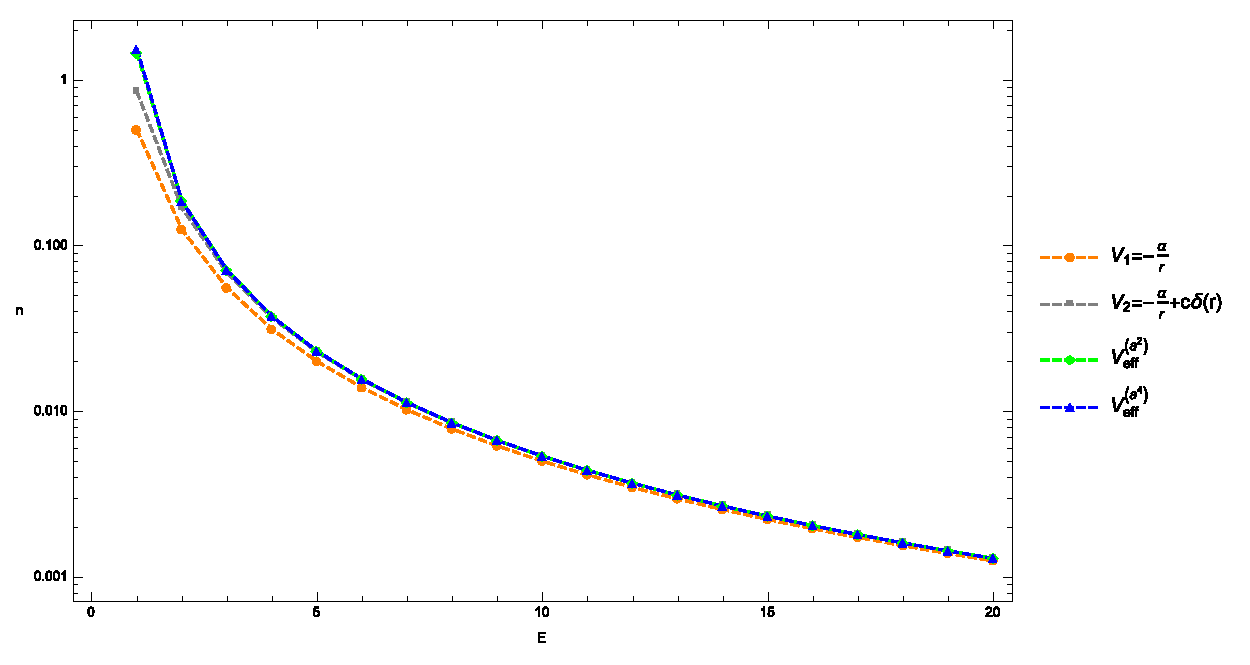
\includegraphics[width=6in]{Test_CurveFitting1_Figure2_1.eps}
  \caption{不同势对应的束缚能}
\end{figure}
\clearpage
\begin{figure}[!htbp]
  \centering
  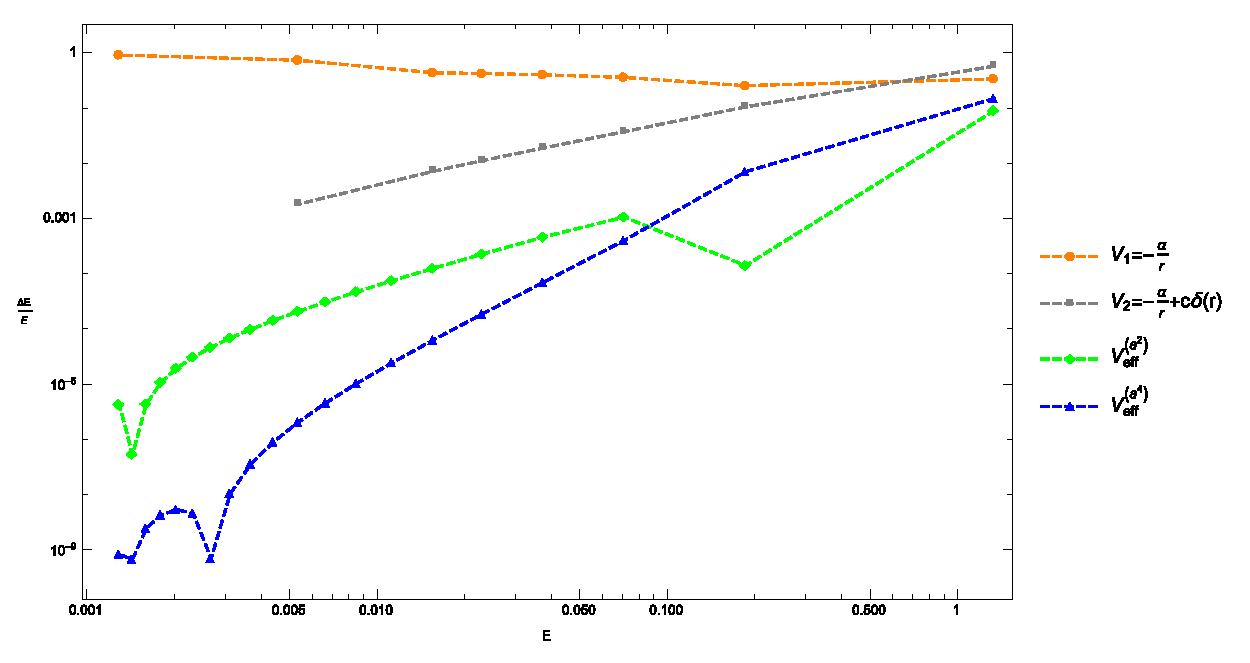
\includegraphics[width=6in]{Test_CurveFitting1_Figure2.eps}
  \caption{不同势对应束缚能的相对误差}
\end{figure}
\subsubsection{利用低能量相移确定系数}
根据之前利用汤川势模型所拟合出的真实势,利用$E=10^{-10}$及$E=10^{-5}$的相移可以确定有效势\eqref{Veffa2}与\eqref{Veffa4}中的系数,同样除了可以假定为观测数据的真实相移外,无需引入其他任何条件。

于是可以得到$c^{(a^2)}=-44.294$以及$c^{(a^4)}=-39.9477$与${d_1}^{(a^4)}=3.26552$。可以看到,利用相移确定的系数与利用束缚能确定的有些微的差别,这一差别是由于求解过程中所采用的准度的评判标准不同而引起的。
\subsubsection{对应束缚能及误差}
由以上确定的系数可以得到对应的束缚能及误差如下图。相比于利用束缚能所确定的系数,这里产生的结果更平滑,没有低能量处的抖动。
\clearpage
\begin{figure}[!htbp]
  \centering
  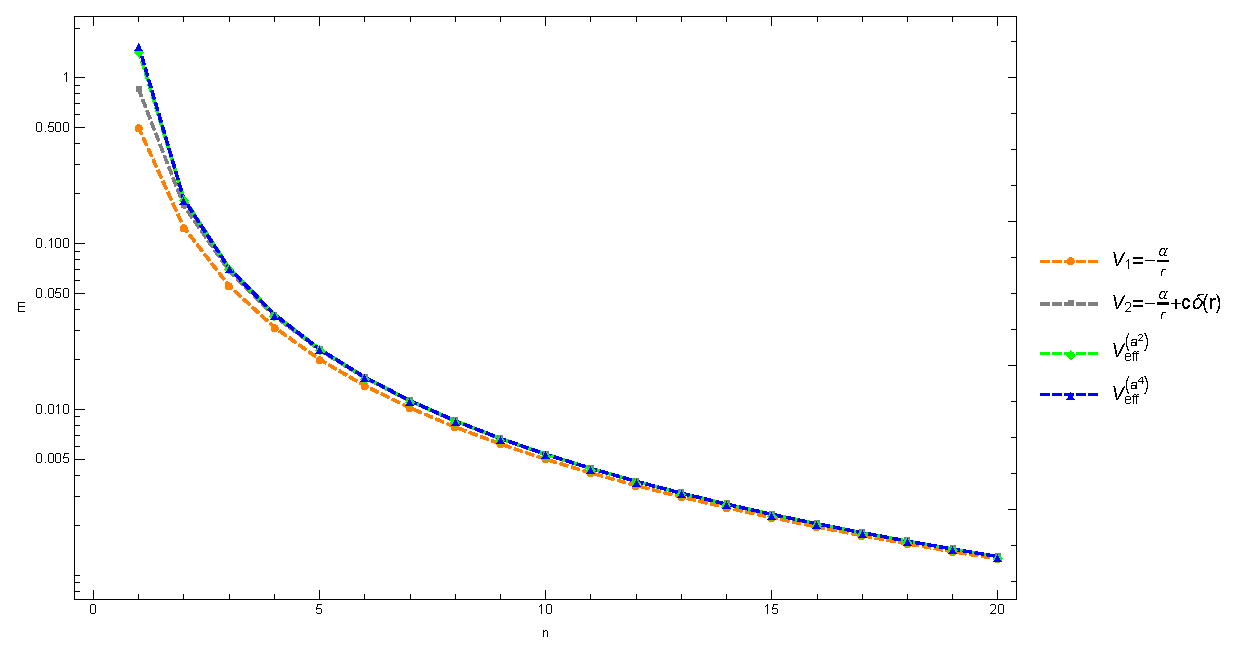
\includegraphics[width=6in]{Test_PS_CurveFitting_Figure2_1.eps}
  \caption{不同势对应的束缚能}
\end{figure}
\begin{figure}[!htbp]
  \centering
  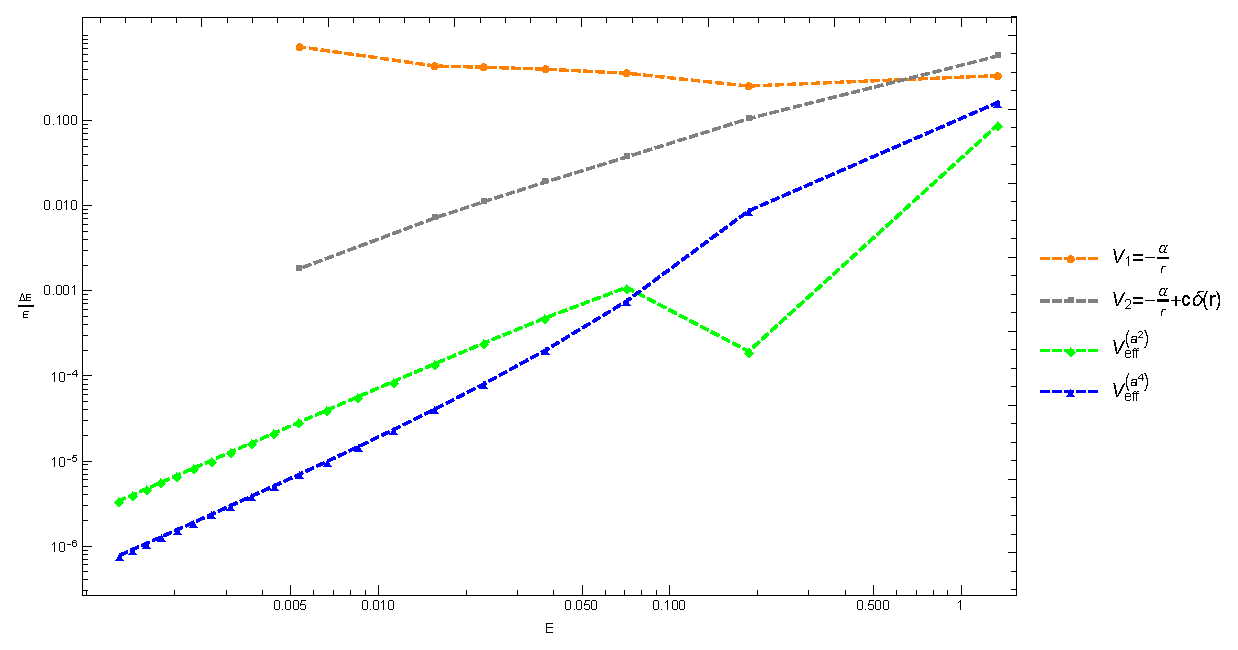
\includegraphics[width=6in]{Test_PS_CurveFitting_Figure2.eps}
  \caption{不同势对应束缚能的相对误差}
\end{figure}
\subsubsection{对应相移及误差}
由以上确定的系数可以得到对应的相移的绝对误差如下图(列入库伦势\eqref{Coulomb}作为对比),有效势的精度显然更高,且有效势的阶数越高,精度越高。\eqref{Veffa4}的相移误差图线中的下陷的原因类似于\eqref{Veffa2}的束缚能误差图线,是由于误差正负号转换引起的。
\begin{figure}[!htbp]
  \centering
  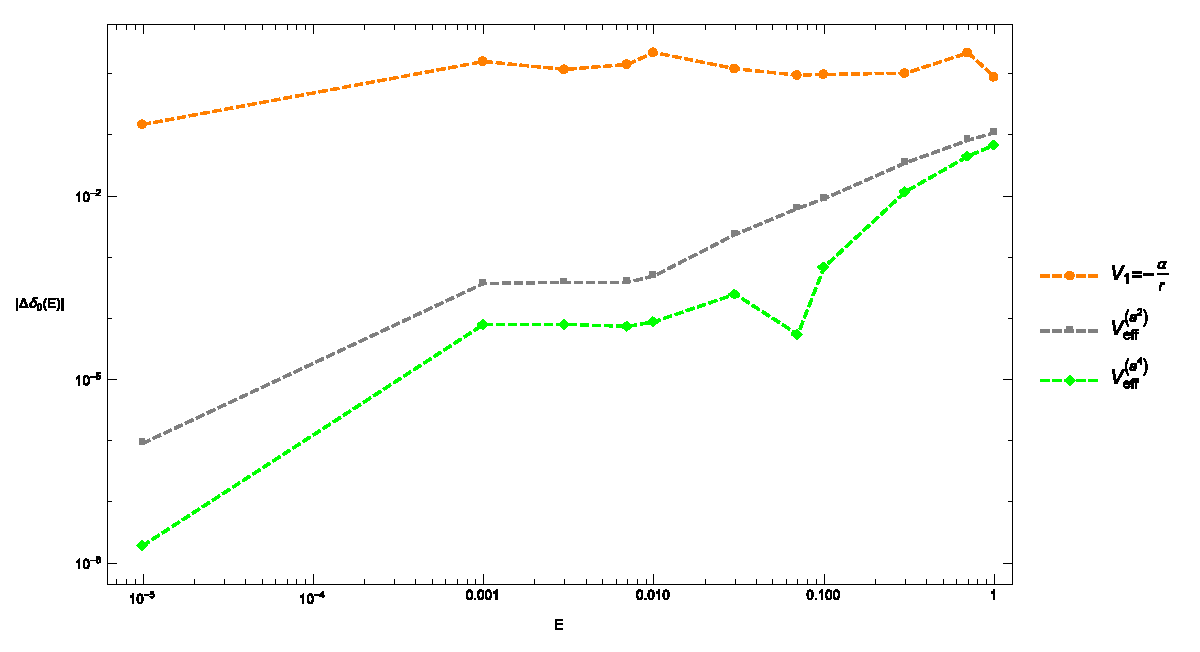
\includegraphics[width=6in]{Test_PS_CurveFitting_Figure3.eps}
  \caption{不同势对应相移的绝对误差}
\end{figure}
\begin{figure}[!htbp]
  \centering
  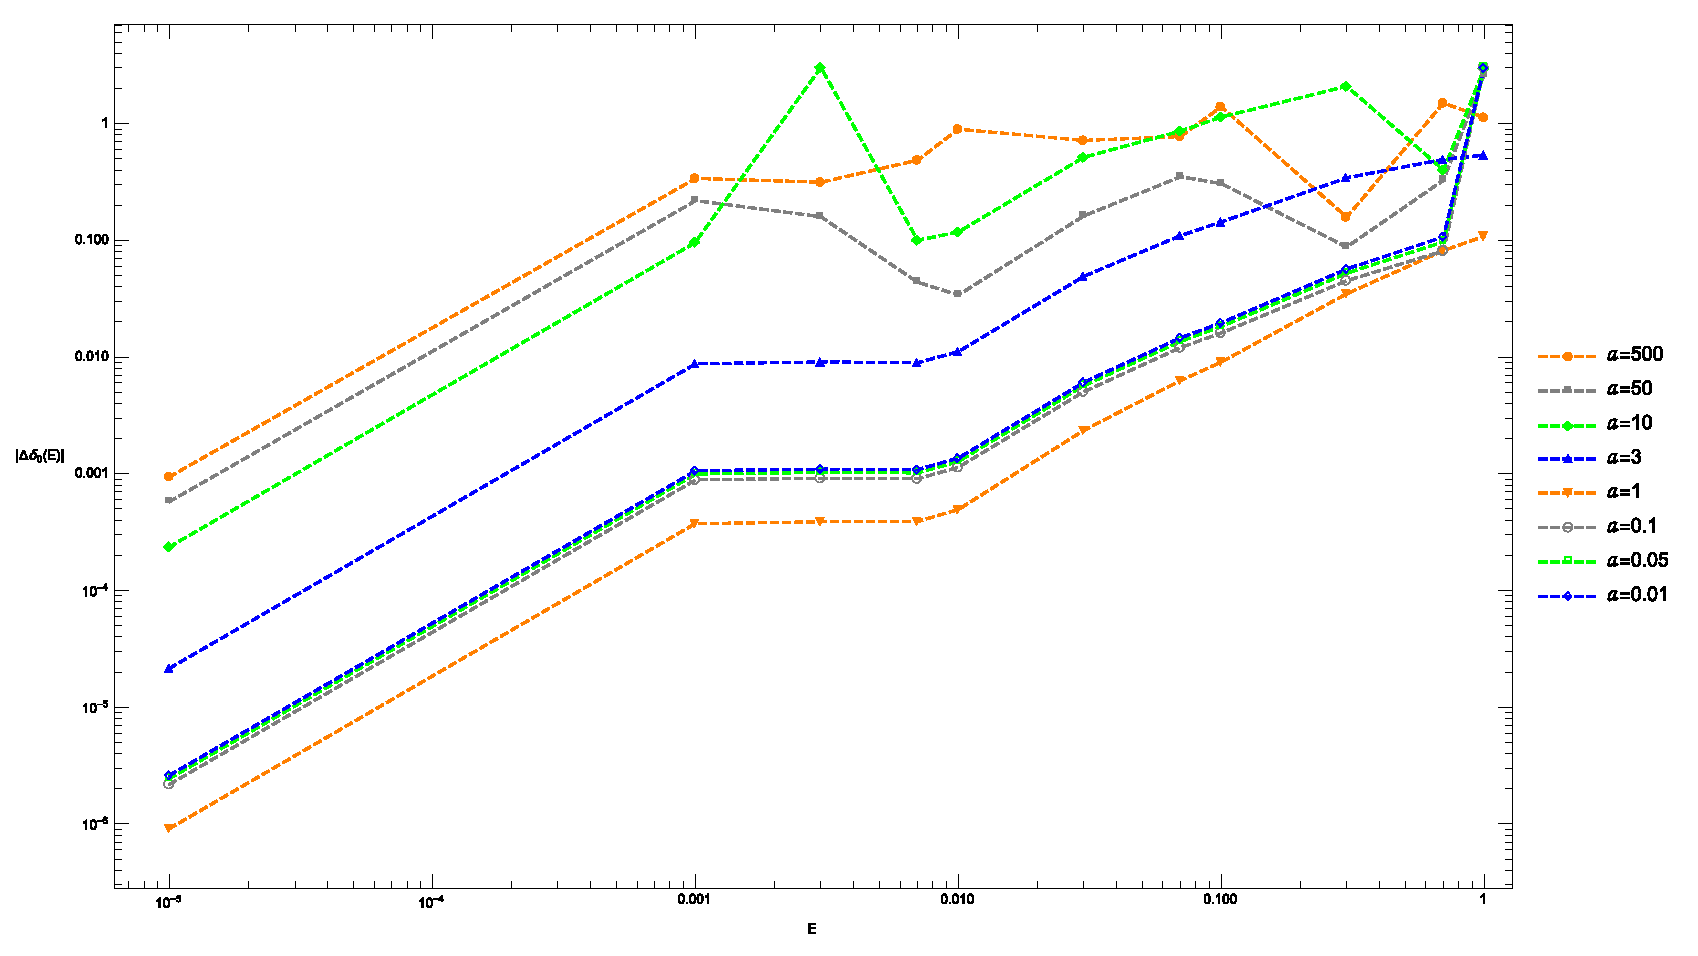
\includegraphics[width=6in]{Test_PhaseShift_Various_a.eps}
  \caption{Cutoff $a$的取值对有效势相移的影响}\label{cutoffa}
\end{figure}
\subsection{\emph{Figure 4}:Cutoff $a$的取值对有效势的影响}
式\eqref{Veffa2}、\eqref{Veffa4}所给出的有效势不仅依赖于$c$、$d1$,还依赖于$a$。之前的计算一直默认$a=1$,但$a$同样也可取其他值。

如图\ref{cutoffa},当$a$取得较大时,有效理论所产生的相移相比于真实相移的相对误差较大;随着$a$的逐渐减小,其相对误差也逐渐减小。当$a$减小到$1$时,相对误差达到最小;如果$a$继续减小,则相对误差又会逐渐增大,但此时其增大的速率会逐渐放缓。由此可见$a=1$更接近于使上述相对误差最小的$a$值。对于之前所讨论的库伦势附加一个汤川势的问题,变换不同的库伦势系数$\alpha$与质量$m$,其最佳的$a$值始终在$1$附近。而问题变到单一的库伦势时,则不能找到一个最佳的$a$值,整体误差随$a$的减小而降低。对于库伦势而言,当$a$变小时,我们的有效势将会逐渐收敛为库伦势:第一项误差函数当$a=0$时显然会变成库伦势,而剩下的局域修正项当$a\rightarrow0$时也将趋于$0$。所以随着$a$的减小,有效势的整体误差会随着减小,但却并不会像附加一个短程势之后那样当$a$小到一定值之后误差反会上扬。这是因为附加了短程势导致$a\rightarrow0$时有效势所收敛到的形式恰是一个库伦势,并不包含对短程势结构的修正,因此误差变高也是可以预期的。
\begin{figure}[!htbp]
\begin{minipage}[t]{0.5\linewidth}
  \centering
  \includegraphics[width=1\textwidth]{{Test_Determine_a_Alpha=0.01&m=10}.eps}
\end{minipage}
\begin{minipage}[t]{0.5\linewidth}
  \centering
  \includegraphics[width=1\textwidth]{{Test_Determine_a_Alpha=0.1&m=1}.eps}
\end{minipage}\\

\begin{minipage}[t]{0.5\linewidth}
  \centering
  \includegraphics[width=1\textwidth]{{Test_Determine_a_Alpha=0.1&m=10}.eps}
\end{minipage}
\begin{minipage}[t]{0.5\linewidth}
  \centering
  \includegraphics[width=1\textwidth]{{Test_Determine_a_Alpha=0.01&m=100}.eps}
\end{minipage}\\

\begin{minipage}[t]{0.5\linewidth}
  \centering
  \includegraphics[width=1\textwidth]{{Test_Determine_a_Alpha=1&m=10}.eps}
\end{minipage}
\begin{minipage}[t]{0.5\linewidth}
  \centering
  \includegraphics[width=1\textwidth]{{Test_Determine_a_Alpha=0.1&m=100}.eps}
\end{minipage}
\caption{库伦势附加短程势$a$的不同取值对有效势相移的影响}
\end{figure}
\begin{figure}[!htbp]
\begin{minipage}[t]{0.5\linewidth}
  \centering
  \includegraphics[width=1\textwidth]{{Test_Determine_Coulomb_a_Alpha=0.01&m=10}.eps}
\end{minipage}
\begin{minipage}[t]{0.5\linewidth}
  \centering
  \includegraphics[width=1\textwidth]{{Test_Determine_Coulomb_a_Alpha=0.1&m=1}.eps}
\end{minipage}\\

\begin{minipage}[t]{0.5\linewidth}
  \centering
  \includegraphics[width=1\textwidth]{{Test_Determine_Coulomb_a_Alpha=0.1&m=10}.eps}
\end{minipage}
\begin{minipage}[t]{0.5\linewidth}
  \centering
  \includegraphics[width=1\textwidth]{{Test_Determine_Coulomb_a_Alpha=0.01&m=100}.eps}
\end{minipage}\\

\begin{minipage}[t]{0.5\linewidth}
  \centering
  \includegraphics[width=1\textwidth]{{Test_Determine_Coulomb_a_Alpha=1&m=10}.eps}
\end{minipage}
\begin{minipage}[t]{0.5\linewidth}
  \centering
  \includegraphics[width=1\textwidth]{{Test_Determine_Coulomb_a_Alpha=0.1&m=100}.eps}
\end{minipage}
\caption{库伦势不附加短程势$a$的不同取值对有效势相移的影响}
\end{figure}
\clearpage
\subsection{有效势的傅里叶变换}
如下式所示:
\begin{eqnarray}
% \nonumber % Remove numbering (before each equation)
  V(\vb{r}) &=& -\frac{1}{r}-\frac{1.04152 e^{-0.9991 r}}{r} \\
  V_{eff}^{(a^2)}(\vb{r}) &=& -\frac{\text{erf}\left(\frac{r}{\sqrt{2}}\right)}{r}-2.81241 e^{-\frac{r^2}{2}} \\
  V_{eff}^{(a^4)}(\vb{r}) &=& -\frac{\text{erf}\left(\frac{r}{\sqrt{2}}\right)}{r}+3.26552 \left(\frac{e^{-\frac{r^2}{2}} r^2}{2 \sqrt{2} \pi ^{3/2}}-\frac{3 e^{-\frac{r^2}{2}}}{2 \sqrt{2} \pi ^{3/2}}\right)-2.53643 e^{-\frac{r^2}{2}}
\end{eqnarray}
有效势与真实势在坐标空间即有较大的差别,二者短程行为并不一致,后者在接近原点处发散,而前者并不发散。
\begin{figure}[!htbp]
  \centering
  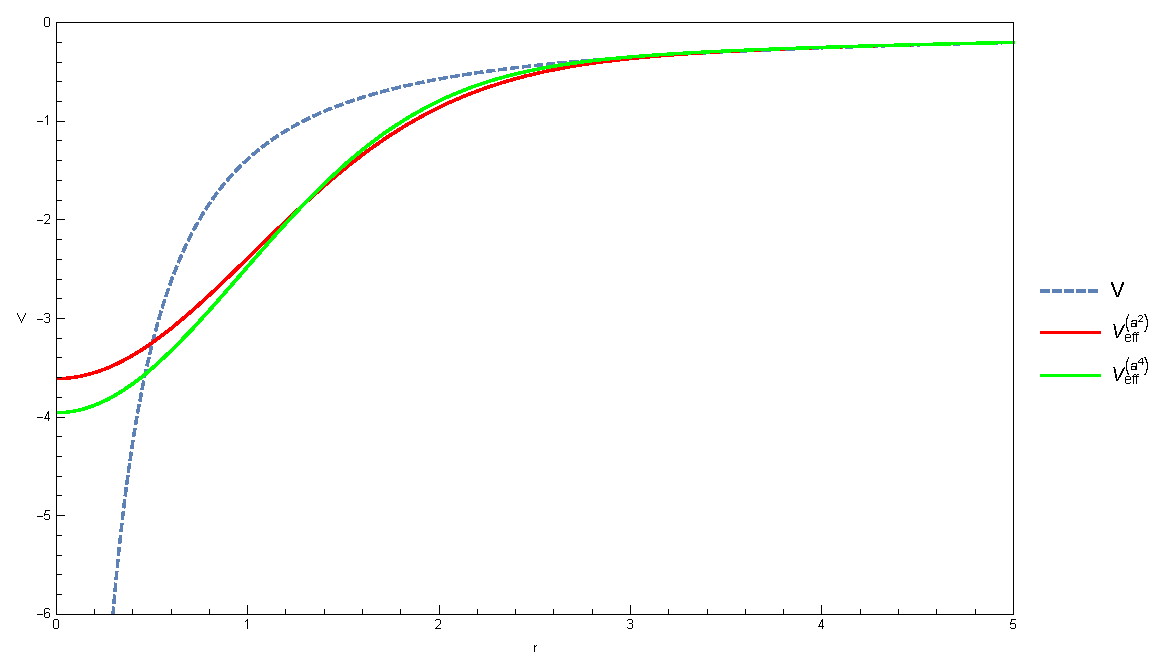
\includegraphics[width=6in]{NoFourierTransformation.eps}
  \caption{有效势与真实势在坐标空间的对比}
\end{figure}\\
将真实势与有效势分别傅里叶变换到动量空间后,其形式如下:
\begin{eqnarray}
% \nonumber % Remove numbering (before each equation)
  v(\vb{k}) &=& -\frac{12.5438}{k^2 \left(k^2+0.998201\right)}-\frac{25.6545}{k^2+0.998201} \\
  v_{eff}^{(a^2)}(\vb{k}) &=& -\frac{12.5664 e^{-0.5 k^2}}{k^2} -44.2944 e^{-0.5 k^2} \\
  v_{eff}^{(a^4)}(\vb{k}) &=& -\frac{12.5664 e^{-0.5 k^2}}{k^2}-3.26552 e^{-0.5 k^2} k^2-39.9477 e^{-0.5 k^2}
\end{eqnarray}
由于动量较大的部分被截断,这部分有效势与真实势的行为出现了极大的差别如图\ref{TotalFourier},而从图像上看,低能行为则趋向一致:
\clearpage
\begin{figure}[!htbp]
  \centering
  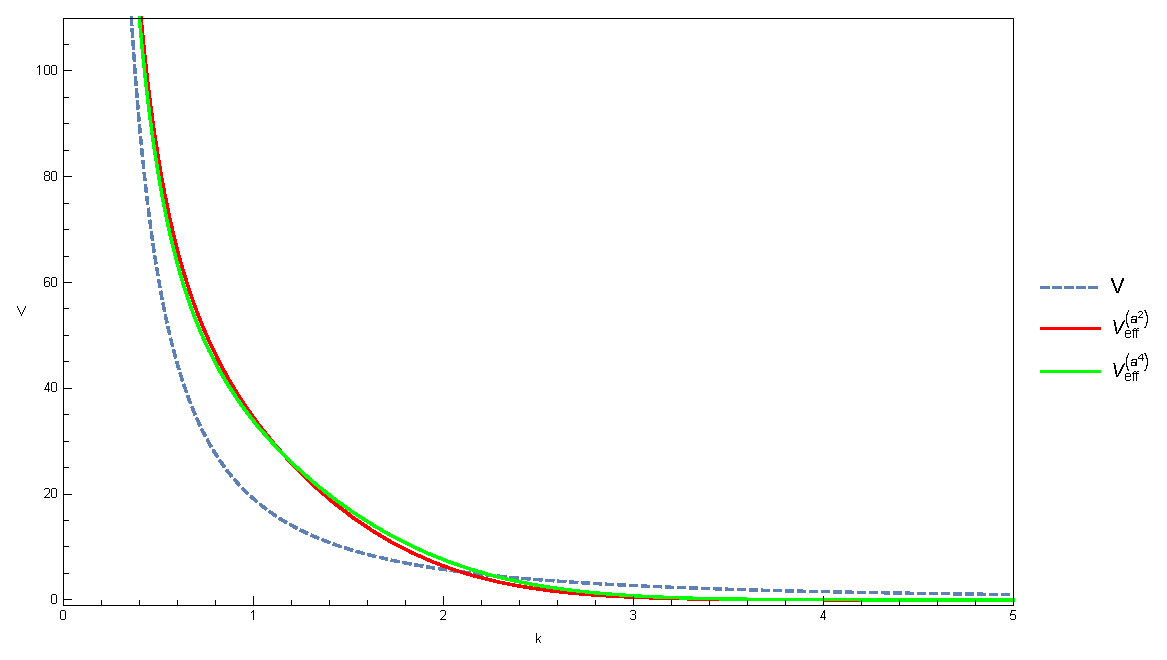
\includegraphics[width=6in]{FourierTransformation_1.eps}
  \caption{有效势与真实势在动量空间的对比}\label{TotalFourier}
\end{figure}
从动量空间的表达式来看,有效势与真实势的第一项较为相似,而真实势的第二项与有效势关于短程部分的修正项则产生了较大差别:
\begin{figure}[!htbp]
  \centering
  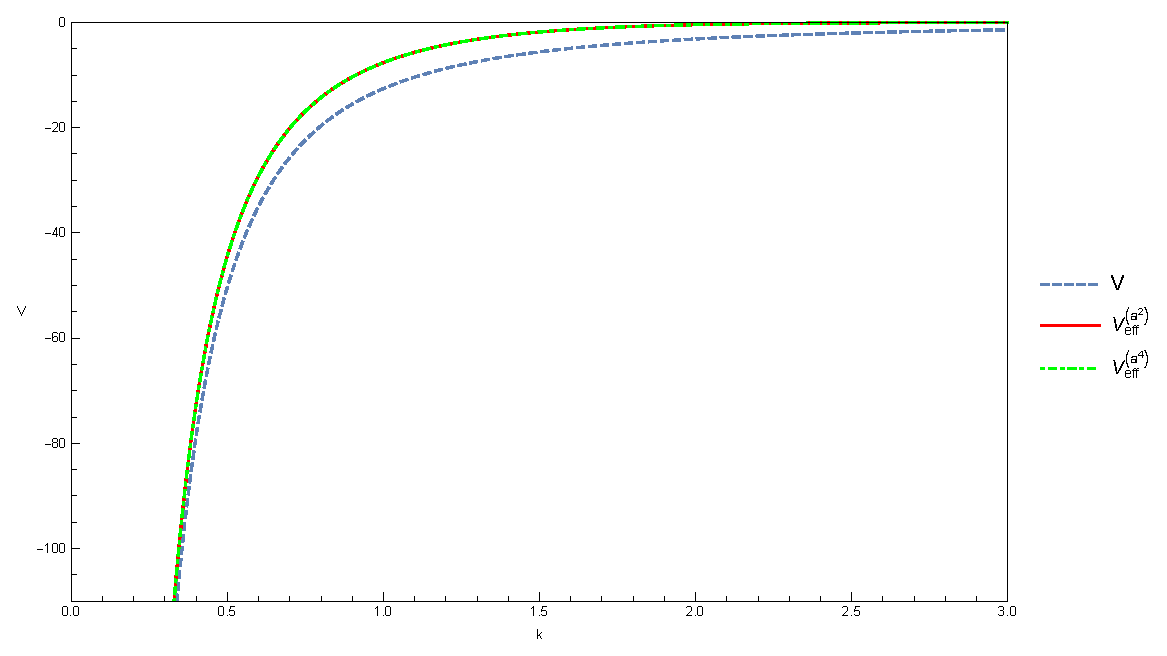
\includegraphics[width=6in]{FourierTransformation_2.eps}
  \caption{有效势与真实势第一项在动量空间的对比}
\end{figure}
\clearpage
\begin{figure}[!htbp]
  \centering
  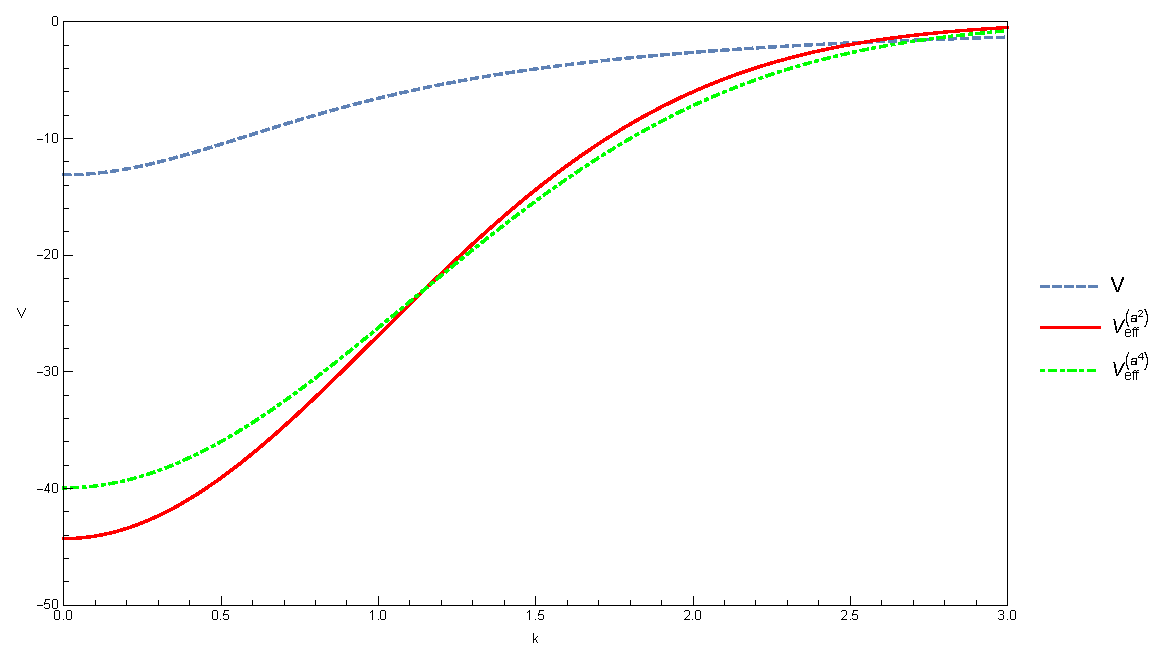
\includegraphics[width=6in]{FourierTransformation_3.eps}
  \caption{有效势与真实势剩余项在动量空间的对比}
\end{figure}
\setlength{\parindent}{0pt}但是当$k\rightarrow0$时,第一项也并不是完全趋于一致的:
\begin{figure}[!htbp]
  \centering
  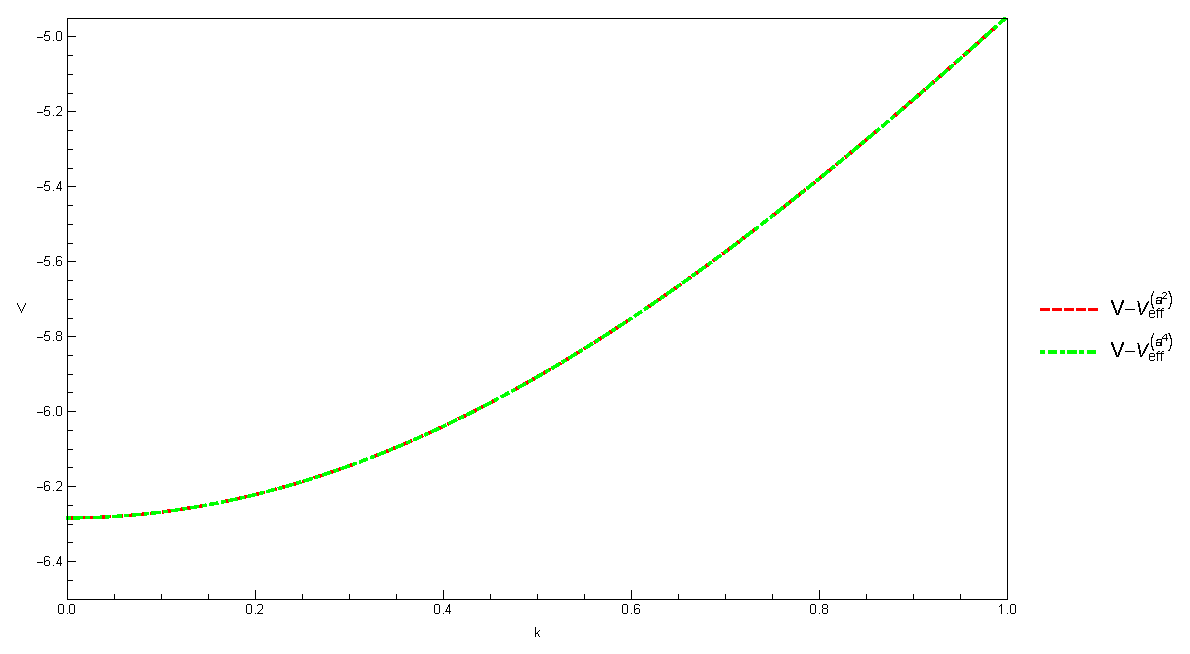
\includegraphics[width=6in]{FourierTransformation_4.eps}
  \caption{真实势与有效势第一项之差在动量空间的对比}
\end{figure}\\
可见即使在动量相比于截断极小时,傅里叶变换后的有效势也并不能收敛到真实势。
\clearpage
\section{矩阵元}
\subsection{$\expval{\vb{p}^4}$}
\subsubsection{利用束缚能确定的有效势}
在真实理论中计算矩阵元$\expval{\vb{p}^4}$,并将之与有效理论($V_{eff}^{(a^4)}$,$a=1$)中的矩阵元$\expval{\vb{p}^4}_{eff}$进行对比,可以发现其差距十分巨大。引入修正,得到以下表达式\cite{Lepage}:
\begin{equation}\label{p4true}
  \expval{\vb{p}^4}_{true}=Z\expval{\vb{p^4}}_{eff}+\frac{\gamma}{a}\expval{\delta^3_a(\vb{r})}_{eff}+\eta a\expval{\laplacian{\delta^3_a(\vb{r})}}_{eff}+\mathcal{O}(a^3)
\end{equation}
并利用10S、15S、20S的真实理论矩阵元确定其系数。得到的系数为$Z=1.26946$、$\gamma=1243.77$与$\eta=82.2527$。于是发现其结果基本与真实理论相符,基态误差较大,能级越高,误差越低。
\begin{table}[!hbtp]
  \centering
  \begin{tabular}{|cccc|}
    \hline
    % after \\: \hline or \cline{col1-col2} \cline{col3-col4} ...
    能级 & $\expval{\vb{p}^4}$ & $\expval{\vb{p^4}}_{eff}$ & $\expval{Z\vb{p}^4+\gamma \delta^3_a/a+\dots}_{eff}$ \\
    \hline
    1S & 75.0651 & 6.16161 & 48.2667 \\
    2S & 5.89805 & 1.79905 & 6.05497 \\
    3S & 1.38388 & 0.454726 & 1.40424 \\
    4S & 0.533537 & 0.179181 & 0.536869 \\
    5S & 0.259685 & 0.0882584 & 0.260443 \\
    6S & 0.145438 & 0.0498093 & 0.145645 \\
    \hline
  \end{tabular}
  \caption{$\expval{\vb{p}^4}$矩阵元在真实势及有效理论中的对比}\label{p4}
\end{table}

为了提高精度,我选取了不同的系数组合,其结果及误差如下图:
\begin{figure}[!htbp]
  \centering
  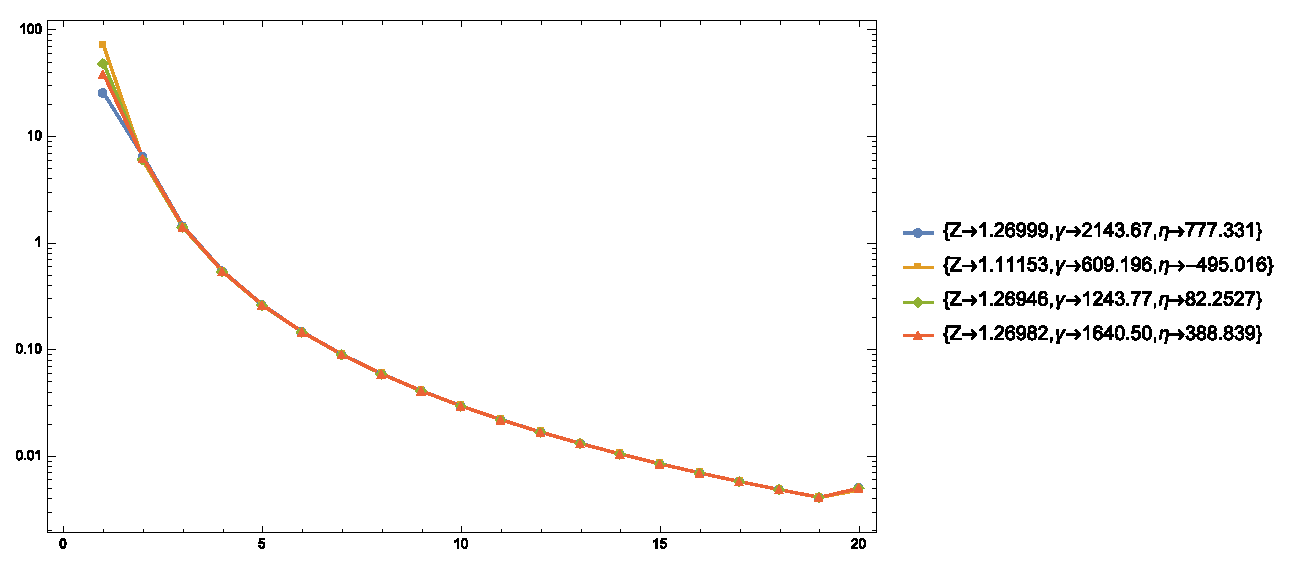
\includegraphics[width=6in]{Test_p4True_2.eps}
  \caption{不同系数组合$\expval{\vb{p}^4}_{true}$的值}\label{p4true pic}
\end{figure}
\begin{figure}[!htbp]
  \centering
  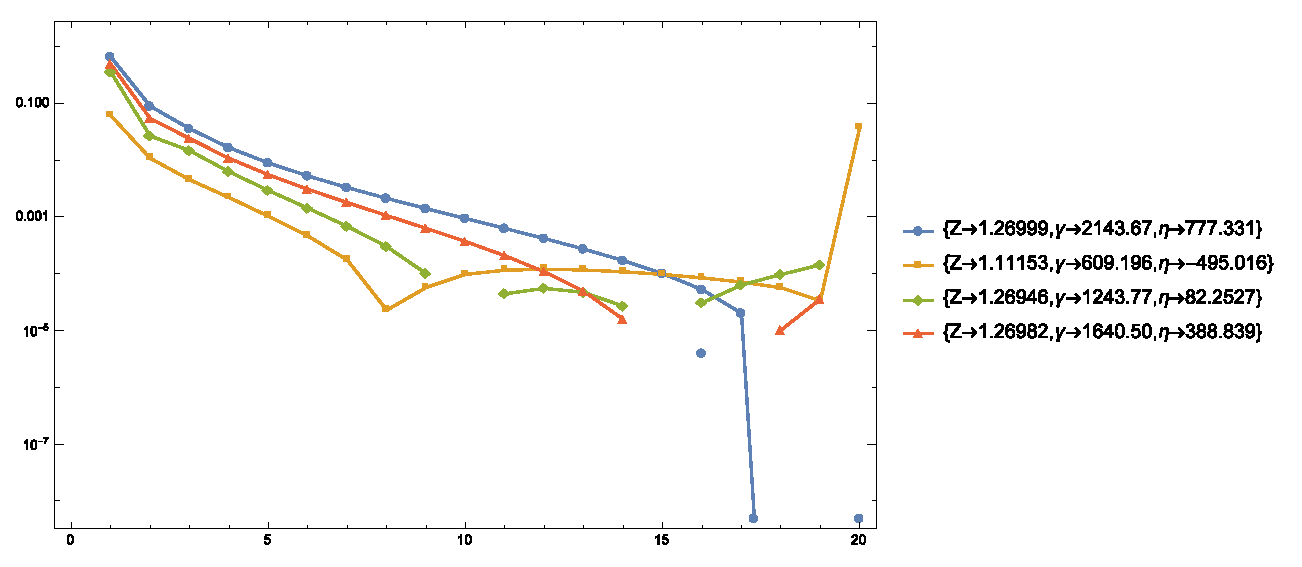
\includegraphics[width=6in]{Test_p4True_2_1.eps}
  \caption{不同系数组合$\expval{\vb{p}^4}_{true}$的相对误差}\label{relative error p4true}
\end{figure}
\subsubsection{利用相移确定的有效势}
由式\eqref{p4true}给出的修正,其中的有效势采用相移所确定的有效势,利用10S、15S、20S的真实理论矩阵元确定其系数,得到$Z=0.988848$、$\gamma=245.680$与$\eta=-851.230$。其结果见表\ref{p41}。
\begin{table}[!hbtp]
  \centering
  \begin{tabular}{|cccccc|}
    \hline
    % after \\: \hline or \cline{col1-col2} \cline{col3-col4} ...
    能级 & $\expval{\vb{p}^4}$ & $\expval{\vb{p^4}}_{eff}$ & $\expval{\vb{p^4}}_{eff}$相对误差 & $\expval{Z\vb{p}^4+\gamma \delta^3_a/a+\dots}_{eff}$ & 修正后相对误差 \\
    \hline
    1S & 75.0651 & 6.39016&0.914872 & 86.2584&0.149114 \\
    2S & 5.89805 & 1.80467&0.694022 & 5.63427&0.0447230 \\
    3S & 1.38388 & 0.459182&0.668193 & 1.37834&0.00400119 \\
    4S & 0.533537 & 0.181115&0.660539 & 0.533006&0.000995149 \\
    5S & 0.259685 & 0.0892336&0.656377 & 0.259594&0.000349898 \\
    6S & 0.145438 & 0.0503636&0.653711 & 0.145417&0.000142768 \\
    7S & 0.0895058 & 0.0311615&0.651849 & 0.895003&0.0000608579 \\
    8S & 0.0589478 & 0.0206038&0.650473 & 0.0589463&0.0000247520 \\
    9S & 0.0408594 & 0.0143248&0.649413 & 0.0408591&$7.89362\times10^{-6}$ \\
    10S& 0.0294762 & 0.0103588 & 0.648572 & 0.0294762 & $0.\times10^{-50}$\\
    11S& 0.0219577 & 0.00773158 & 0.647888 & 0.0219578 & $2.86723\times10^{-6}$\\
    12S& 0.0167936 & 0.00592277 & 0.647320 & 0.0167937 & $3.65482\times10^{-6}$\\
    13S& 0.0131299 & 0.00463692 & 0.646842 & 0.0131299 & $3.06033\times10^{-6}$\\
    14S& 0.0104589 & 0.00369791 & 0.646433 & 0.0104589 & $1.68057\times10^{-6}$\\
    15S& 0.00846592 & 0.00299626 & 0.646080 & 0.00846592 &  $0.\times10^{-50}$\\
    16S& 0.00694880 & 0.00246146 & 0.645772 & 0.00694878 & $1.78021\times10^{-6}$\\
    17S& 0.00577356 & 0.00204673 & 0.645500 & 0.00577354 & $3.67384\times10^{-6}$\\
    18S& 0.00484908 & 0.00172016 & 0.645260 & 0.00484906 & $5.47461\times10^{-6}$\\
    19S& 0.00411194 & 0.00145962 & 0.645029 & 0.00411195 & $2.37062\times10^{-6}$\\
    20S& 0.00503698 & 0.00278627 & 0.446837 & 0.00503698 & $0.\times10^{-50}$\\
    \hline
  \end{tabular}
  \caption{$\expval{\vb{p}^4}$矩阵元在真实势及有效理论(相移)中的对比}\label{p41}
\end{table}
\subsection{$\displaystyle\expval{\frac{1}{r}}$}
\subsubsection{利用束缚能确定的有效势}
类似于$\expval{\vb{p}^4}$,$\displaystyle\expval{\frac{1}{r}}$具备同样的表现。修正后的表达式为:
\begin{equation}\label{rtrue}
  \expval{\frac{1}{r}}_{true}=Z\expval{\frac{1}{r}}_{eff}+\frac{\gamma}{a}\expval{\delta^3_a(\vb{r})}_{eff}+\eta a\expval{\laplacian{\delta^3_a(\vb{r})}}_{eff}+\mathcal{O}(a^3)
\end{equation}
修正项系数为$Z=1.00001$、$\gamma=-14.6632$与$\eta= -13.1376$。 从下表可以看出,相比于$\expval{\vb{p}^4}$,$\displaystyle\expval{\frac{1}{r}}$的有效理论在未经修正时的误差相对较小,但修正后仍大幅降低了这一误差。
\begin{table}[!hbtp]
  \centering
  \begin{tabular}{|cccccc|}
    \hline
    % after \\: \hline or \cline{col1-col2} \cline{col3-col4} ...
    能级 & $\expval{1/r}$ & $\expval{1/r}_{eff}$ & $\expval{1/r}_{eff}$ 相对误差& $\expval{Z/r+\gamma \delta^3_a/a+\dots}_{eff}$ & 修正后相对误差 \\
    \hline
    1S & 1.92548 & 1.27796 &0.336292& 1.79727&0.0665873 \\
    2S & 0.351169 & 0.345255 &0.0168427& 0.345975&0.0147922 \\
    3S & 0.136034 & 0.134806 &0.00902901& 0.13596&0.000546773 \\
    4S & 0.0724346 & 0.0718963 &0.00743124& 0.0724315&0.0000425632 \\
    5S & 0.0449404 & 0.0446631 &0.00617019& 0.0449405&$3.91509^{-6}$ \\
    6S & 0.0305861 & 0.0304262 &0.00522542& 0.0305863&$6.28028^{-6}$ \\
    \hline
  \end{tabular}
  \caption{$\displaystyle\expval{\frac{1}{r}}$矩阵元在真实势及有效理论中的对比}\label{evr}
\end{table}
\subsubsection{利用相移确定的有效势}
由式\eqref{rtrue}给出的修正,其中的有效势采用相移所确定的有效势,利用10S、15S、20S的真实理论矩阵元确定其系数,得到$Z=0.999998$、$\gamma=-12.36$与$\eta=-11.4262$。
\begin{table}[!hbtp]
  \centering
  \begin{tabular}{|cccccc|}
    \hline
    % after \\: \hline or \cline{col1-col2} \cline{col3-col4} ...
    能级 & $\expval{1/r}$ & $\expval{1/r}_{eff}$ & $\expval{1/r}_{eff}$ 相对误差& $\expval{Z/r+\gamma \delta^3_a/a+\dots}_{eff}$ & 修正后相对误差 \\
    \hline
    1S & 1.92548 & 1.28960 &0.330244& 1.7642&0.0837596 \\
    2S & 0.351169 & 0.344153 &0.0199786& 0.345096&0.0172951 \\
    3S & 0.136034 & 0.134796 &0.00909973& 0.135905&0.00094791 \\
    4S & 0.0724346 & 0.0719137 &0.00719131& 0.0724226&0.000165167 \\
    5S & 0.0449404 & 0.0446755 &0.00589443& 0.0449384&$0.0000438437$ \\
    6S & 0.0305861 & 0.0304343 &0.00496313& 0.0305856&$0.0000143115$ \\
    \hline
  \end{tabular}
  \caption{$\displaystyle\expval{\frac{1}{r}}$矩阵元在真实势及有效理论(相移)中的对比}\label{evr1}
\end{table}
\subsection{$\displaystyle\expval{\frac{1}{r^2}}$}
\subsubsection{利用束缚能确定的有效势}
$\displaystyle\expval{\frac{1}{r^2}}$的有效理论修正后的表达式为:
\begin{equation}\label{r2true}
  \expval{\frac{1}{r^2}}_{true}=Z\expval{\frac{1}{r^2}}_{eff}+\frac{\gamma}{a}\expval{\delta^3_a(\vb{r})}_{eff}+\eta a\expval{\laplacian{\delta^3_a(\vb{r})}}_{eff}+\mathcal{O}(a^3)
\end{equation}
修正项系数为$Z=7.14984$、$\gamma=-206.7$与$\eta=329.741$。对于这一矩阵元,最大的问题在于基态的值上;未经修正的有效理论在基态上误差比修正后还小。但是未经修正的值在之后的几个能级上误差基本不变,而修正后误差则快速降低。
\begin{table}[!hbtp]
  \centering
  \begin{tabular}{|cccccc|}
    \hline
    % after \\: \hline or \cline{col1-col2} \cline{col3-col4} ...
    能级 & $\expval{1/r^2}$ & $\expval{1/r^2}_{eff}$ & $\expval{1/r^2}_{eff}$ 相对误差& $\expval{Z/r^2+\gamma \delta^3_a/a+\dots}_{eff}$ & 修正后相对误差 \\
    \hline
    1S & 7.54675 & 2.64833 &0.649077& -15.8996&3.10682 \\
    2S & 0.513020 & 0.338657 &0.339876& 0.519597&0.0128214 \\
    3S & 0.117680 & 0.0787820 &0.330541& 0.11814&0.00391092 \\
    4S & 0.0448732 & 0.0299838 &0.331810& 0.0449209&0.00106295 \\
    5S & 0.0217022 & 0.0144860 &0.332509& 0.02171&0.000359689 \\
    6S & 0.0121042 & 0.00807484 &0.332891& 0.0121059&0.000136607 \\
    \hline
  \end{tabular}
  \caption{$\displaystyle\expval{\frac{1}{r^2}}$矩阵元在真实势及有效理论中的对比}\label{evr2}
\end{table}
\subsubsection{利用相移确定的有效势}
由式\eqref{r2true}给出的修正,其中的有效势采用相移所确定的有效势,利用10S、15S、20S的真实理论矩阵元确定其系数,得到$Z=0.879922$、$\gamma=7.98866$与$\eta=-48.2468$。
\begin{table}[!hbtp]
  \centering
  \begin{tabular}{|cccccc|}
    \hline
    % after \\: \hline or \cline{col1-col2} \cline{col3-col4} ...
    能级 & $\expval{1/r^2}$ & $\expval{1/r^2}_{eff}$ & $\expval{1/r^2}_{eff}$ 相对误差& $\expval{Z/r^2+\gamma \delta^3_a/a+\dots}_{eff}$ & 修正后相对误差 \\
    \hline
    1S & 7.54675 & 2.69689 &0.642641& 6.67706&0.115240 \\
    2S & 0.513020 & 0.336075 &0.344909& 0.494684&0.0357409 \\
    3S & 0.117680 & 0.0787285 &0.330996& 0.117379&0.00255816 \\
    4S & 0.0448732 & 0.0300000 &0.331449& 0.0448488&0.000542838 \\
    5S & 0.0217022 & 0.0144998 &0.331875& 0.0216986&0.000167238 \\
    6S & 0.0121042 & 0.00808401 &0.332134& 0.0121035&0.0000609963 \\
    \hline
  \end{tabular}
  \caption{$\displaystyle\expval{\frac{1}{r^2}}$矩阵元在真实势及有效理论(相移)中的对比}\label{evr21}
\end{table}
\subsection{$\displaystyle\expval{\frac{1}{r^3}}$}
\subsubsection{利用束缚能确定的有效势}
$\displaystyle\expval{\frac{1}{r^3}}$的有效理论修正后的表达式为:
\begin{equation}\label{r3true}
  \expval{\frac{1}{r^3}}_{true}=Z\expval{\frac{1}{r^3}}_{eff}+\frac{\gamma}{a}\expval{\delta^3_a(\vb{r})}_{eff}+\eta a\expval{\laplacian{\delta^3_a(\vb{r})}}_{eff}+\mathcal{O}(a^3)
\end{equation}
修正项系数为$Z=-28.2863$、$\gamma=1.334\times10^6$与$\eta=-1.722\times10^6$。
\begin{table}[!hbtp]
  \centering
  \begin{tabular}{|cccccc|}
    \hline
    % after \\: \hline or \cline{col1-col2} \cline{col3-col4} ...
    能级 & $\expval{1/r^3}$ & $\expval{1/r^3}_{eff}$ & $\expval{1/r^3}_{eff}$ 相对误差& $\expval{Z/r^3+\gamma \delta^3_a/a+\dots}_{eff}$ & 修正后相对误差 \\
    \hline
    1S & 21319.2 & 2549.00 &0.880436& 119482&4.60443 \\
    2S & 1369.00 & 338.751 &0.752555& 1183.99&0.135143 \\
    3S & 310.592 & 77.9955 &0.748881& 302.84&0.0249606 \\
    4S & 118.122 & 29.5950 &0.749453& 116.967&0.00977874 \\
    5S & 57.0661 & 14.3001 &0.749412& 56.2036&0.0151141 \\
    6S & 31.8107 & 7.94969 &0.750094& 31.8548&0.00138628 \\
    \hline
  \end{tabular}
  \caption{$\displaystyle\expval{\frac{1}{r^3}}$矩阵元在真实势及有效理论中的对比}\label{evr3}
\end{table}\\
$\expval{\frac{1}{r^3}}$的被积函数在接近0处出现了较明显的奇异性,积分上遇到了困难。对于更高次的算符则更加明显,例如$\expval{\frac{1}{r^4}}$,积分出现发散。
\subsubsection{利用相移确定的有效势}
由式\eqref{r3true}给出的修正,其中的有效势采用相移所确定的有效势,对积分策略稍作修正,利用10S、15S、20S的真实理论矩阵元确定其系数,得到$Z=-1.88313$、$\gamma=252685$与$\eta=-311567$。
\begin{table}[!hbtp]
  \centering
  \begin{tabular}{|cccccc|}
    \hline
    % after \\: \hline or \cline{col1-col2} \cline{col3-col4} ...
    能级 & $\expval{1/r^3}$ & $\expval{1/r^3}_{eff}$ & $\expval{1/r^3}_{eff}$ 相对误差& $\expval{Z/r^3+\gamma \delta^3_a/a+\dots}_{eff}$ & 修正后相对误差 \\
    \hline
    1S & 21261.3 & 2612.36 &0.877131& 30560.7&0.437390 \\
    2S & 1365.28 & 336.763 &0.753337& 1302.27&0.0461507 \\
    3S & 309.748 & 78.1585 &0.747671& 308.562&0.00382939 \\
    4S & 117.801 & 29.6996 &0.747882& 117.700&0.000849579 \\
    5S & 56.9110 & 14.3375 &0.748072& 56.8958&0.000265940 \\
    6S & 31.7243 & 7.98857 &0.748187& 31.7212&0.0000974506 \\
    \hline
  \end{tabular}
  \caption{$\displaystyle\expval{\frac{1}{r^3}}$矩阵元在真实势及有效理论中的对比}\label{evr31}
\end{table}
\subsection{$\psi(0)$}
\subsubsection{利用束缚能确定的有效势}
$\psi_{eff}(0)$修正后表达式为:
\begin{equation}\label{psi0}
  \psi_{true}(0)=\overline{\gamma}\int\dd^3r\psi_{eff}\delta^3_a(\vb{r})+\overline{\eta}a^2\int\dd^3r\psi_{eff}\laplacian{\delta^3_a(\vb{r})}+\mathcal{O}(a^3)
\end{equation}
\begin{table}[!hbtp]
  \centering
  \begin{tabular}{|cccccc|}
    \hline
    % after \\: \hline or \cline{col1-col2} \cline{col3-col4} ...
    能级 & $\psi(0)$ & $\psi_{eff}(0)$ & $\psi_{eff}(0)$ 相对误差& $\overline{\gamma}\int\psi_{eff}\delta^3_a+\dots$ & 修正后相对误差 \\
    \hline
    1S & -1.54924 & -0.535135 &0.654583& 3.81087&3.45983 \\
    2S & -0.392598 & -0.195113 &0.503021& -0.378348&0.0362967 \\
    3S & -0.187001 & -0.0936242 &0.499339& -0.186402&0.00320329 \\
    4S & 0.115323 & 0.0576719 &0.499908& 0.115252&0.000609275 \\
    5S & 0.0801566 & 0.0400607 &0.500219& 0.0801461&0.000130787 \\
    6S & -0.0598462 & -0.0298998 &0.50039& -0.0598455&0.0000122656 \\
    \hline
  \end{tabular}
  \caption{$\psi(0)$在真实势及有效理论中的对比}
\end{table}
\subsubsection{利用相移确定的有效势}
由式\eqref{psi0}给出的修正,其中的有效势采用相移所确定的有效势,利用15S、20S的真实理论$\psi(0)$确定其系数,得到$\overline{\gamma}=-30.3085$与$\overline{\eta}=-3.07358$。
\clearpage
\begin{table}[!htbp]
  \centering
  \begin{tabular}{|cccccc|}
    \hline
    % after \\: \hline or \cline{col1-col2} \cline{col3-col4} ...
    能级 & $\psi(0)$ & $\psi_{eff}(0)$ & $\psi_{eff}(0)$ 相对误差& $\overline{\gamma}\int\psi_{eff}\delta^3_a+\dots$ & 修正后相对误差 \\
    \hline
    1S & -1.54924 & -0.542484 &0.64984& 3.76435&3.42979 \\
    2S & -0.392598 & -0.194805 &0.503805& -0.378129&0.0368562 \\
    3S & -0.187001 & -0.0938498 &0.498132& -0.186388&0.00327793 \\
    4S & 0.115323 & 0.0578526 &0.498341& 0.115252&0.000614599 \\
    5S & 0.0801566 & 0.0401962 &0.498529& 0.0801468&0.000122377 \\
    6S & -0.0598462 & -0.0300043 &0.498643& -0.0598461&$1.89745\times10^{-6}$ \\
    \hline
  \end{tabular}
  \caption{$\psi(0)$在真实势及有效理论(相移)中的对比}\label{psi01}
\end{table}
\subsection{$\psi(r)$}
$\psi_{eff}(r)$修正后表达式为:
\begin{equation}\label{psi0r}
  \psi_{true}(r)=\overline{\gamma}(r)\int\dd^3r\psi_{eff}\delta^3_a(\vb{r})+\overline{\eta}(r)a^2\int\dd^3r\psi_{eff}\laplacian{\delta^3_a(\vb{r})}+\mathcal{O}(a^3)
\end{equation}
这一关系仅在$r<a$时成立。
\begin{figure}[!htbp]
  \centering
  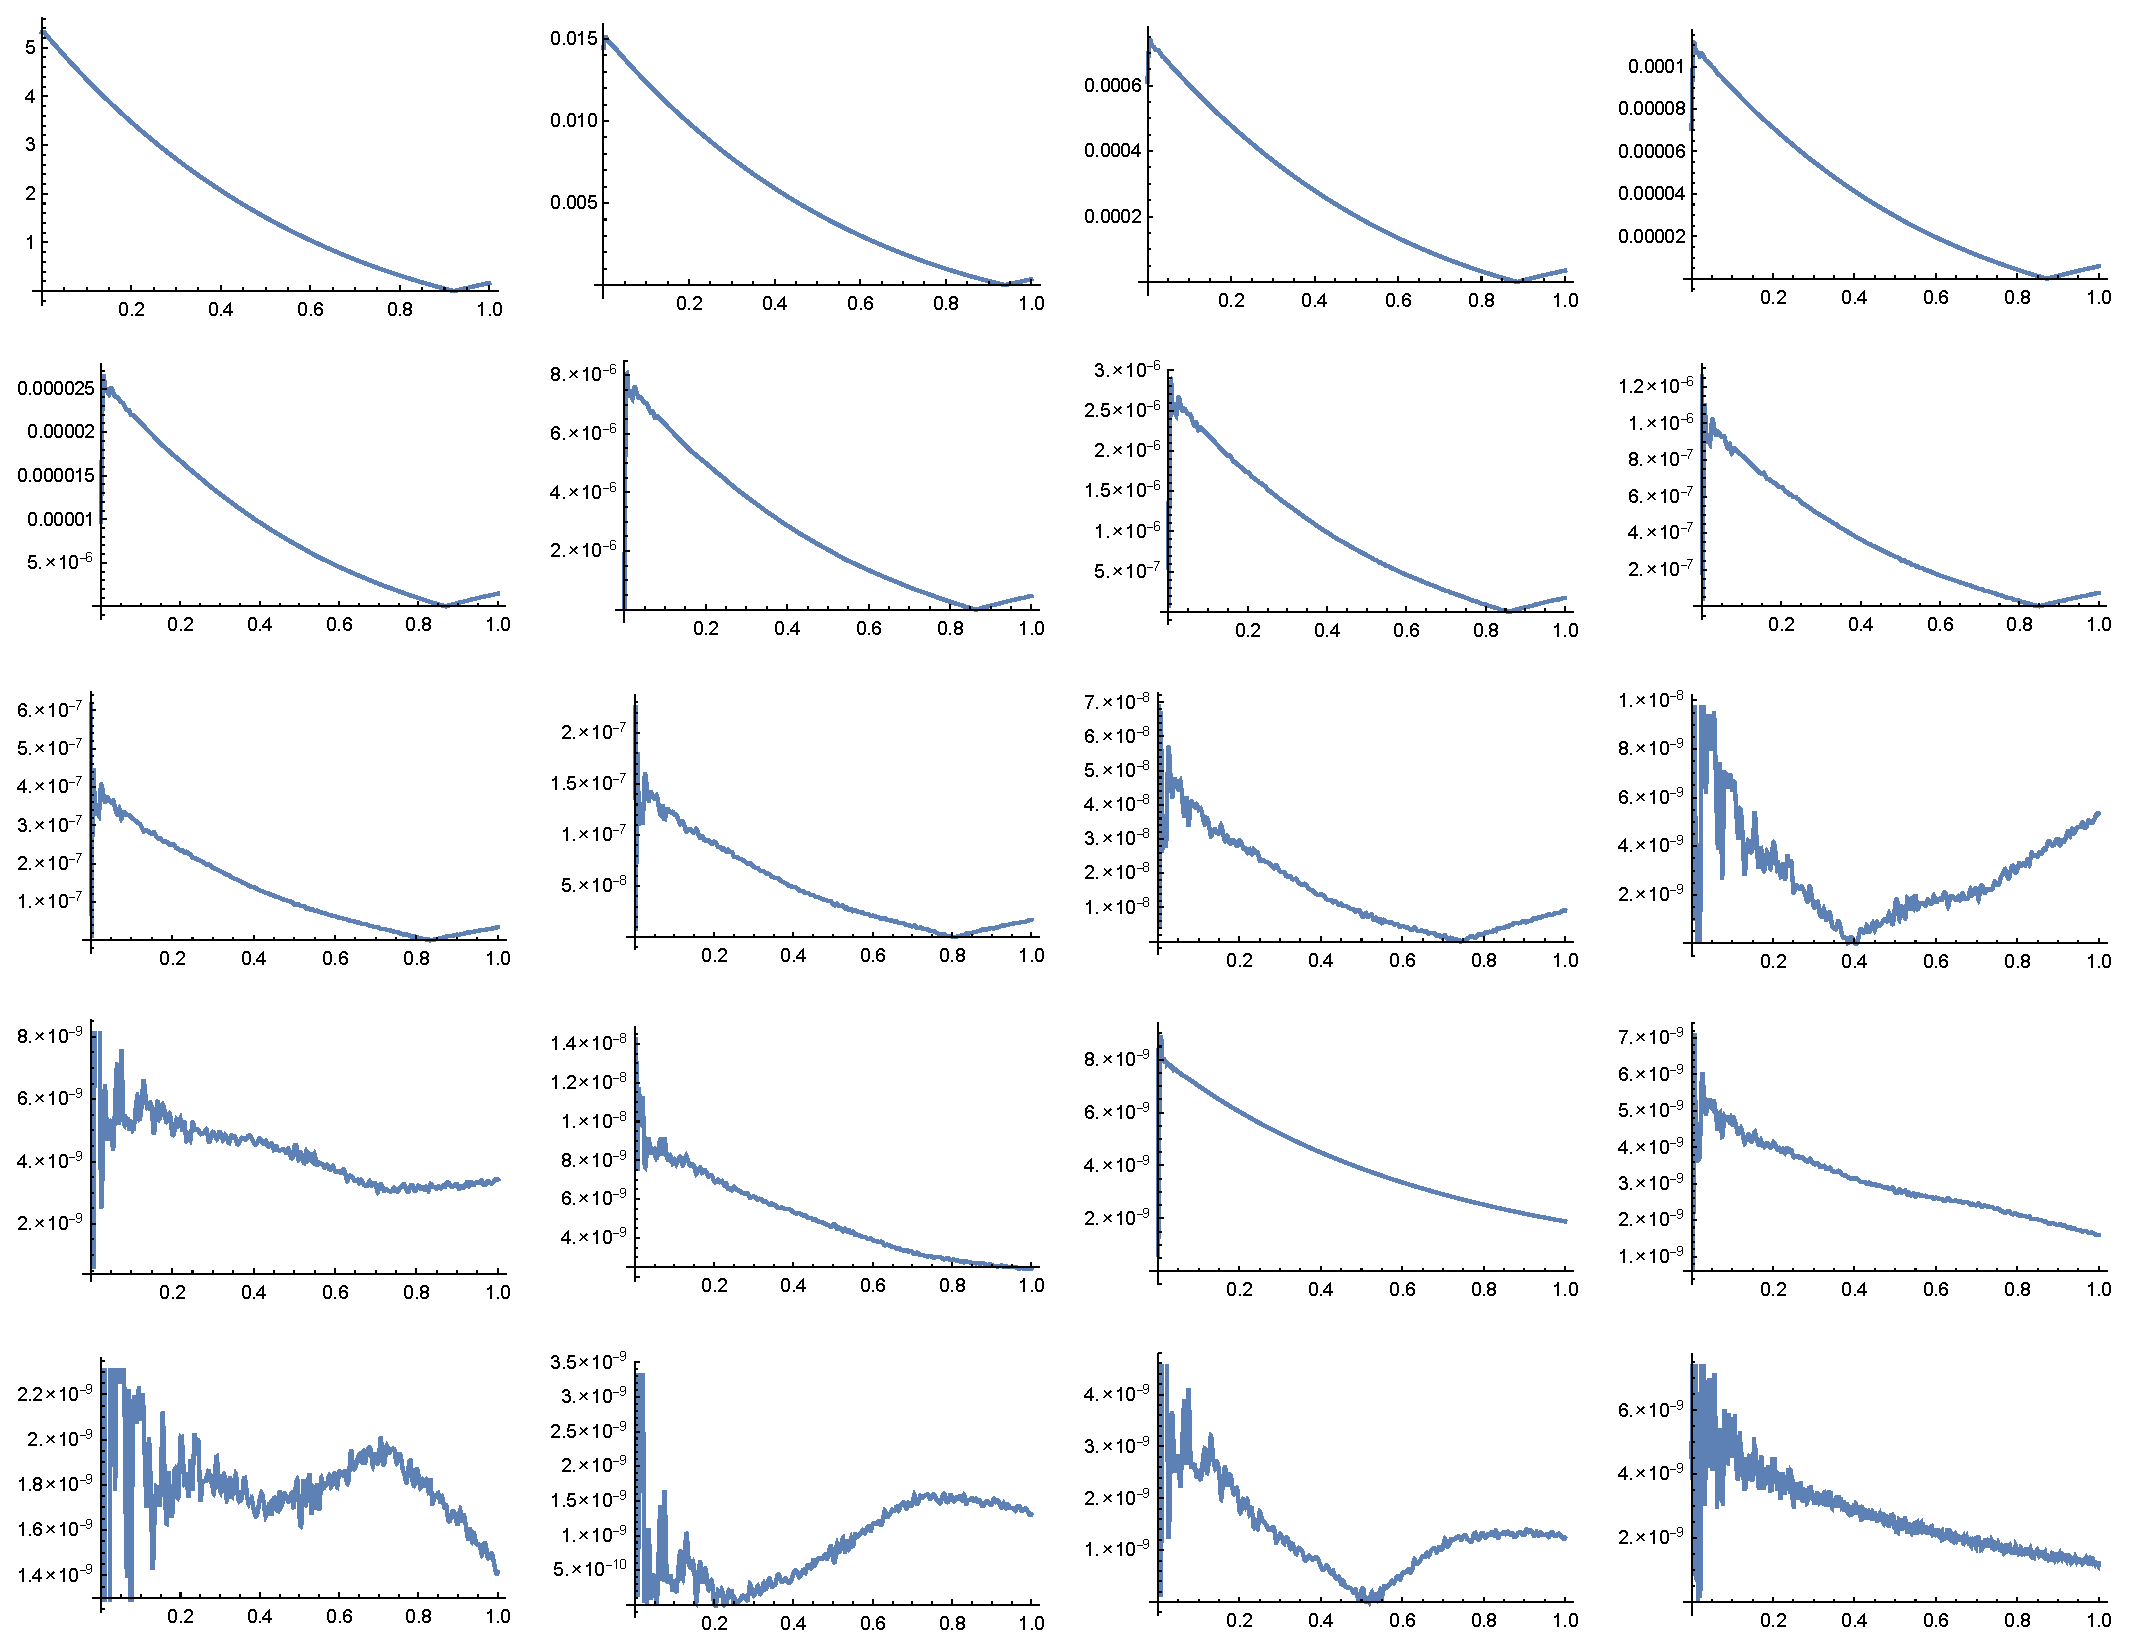
\includegraphics[width=6in]{psir.eps}
  \caption{$\psi_{eff}(r)$在前20个能级与真实波函数的对比}
\end{figure}\\
可以发现除了第一个能级之外,其它能级与真实波函数都符合得较好,并且能级越高,符合得越好。若$r>a$,则
\clearpage
\begin{figure}[!htbp]
  \centering
  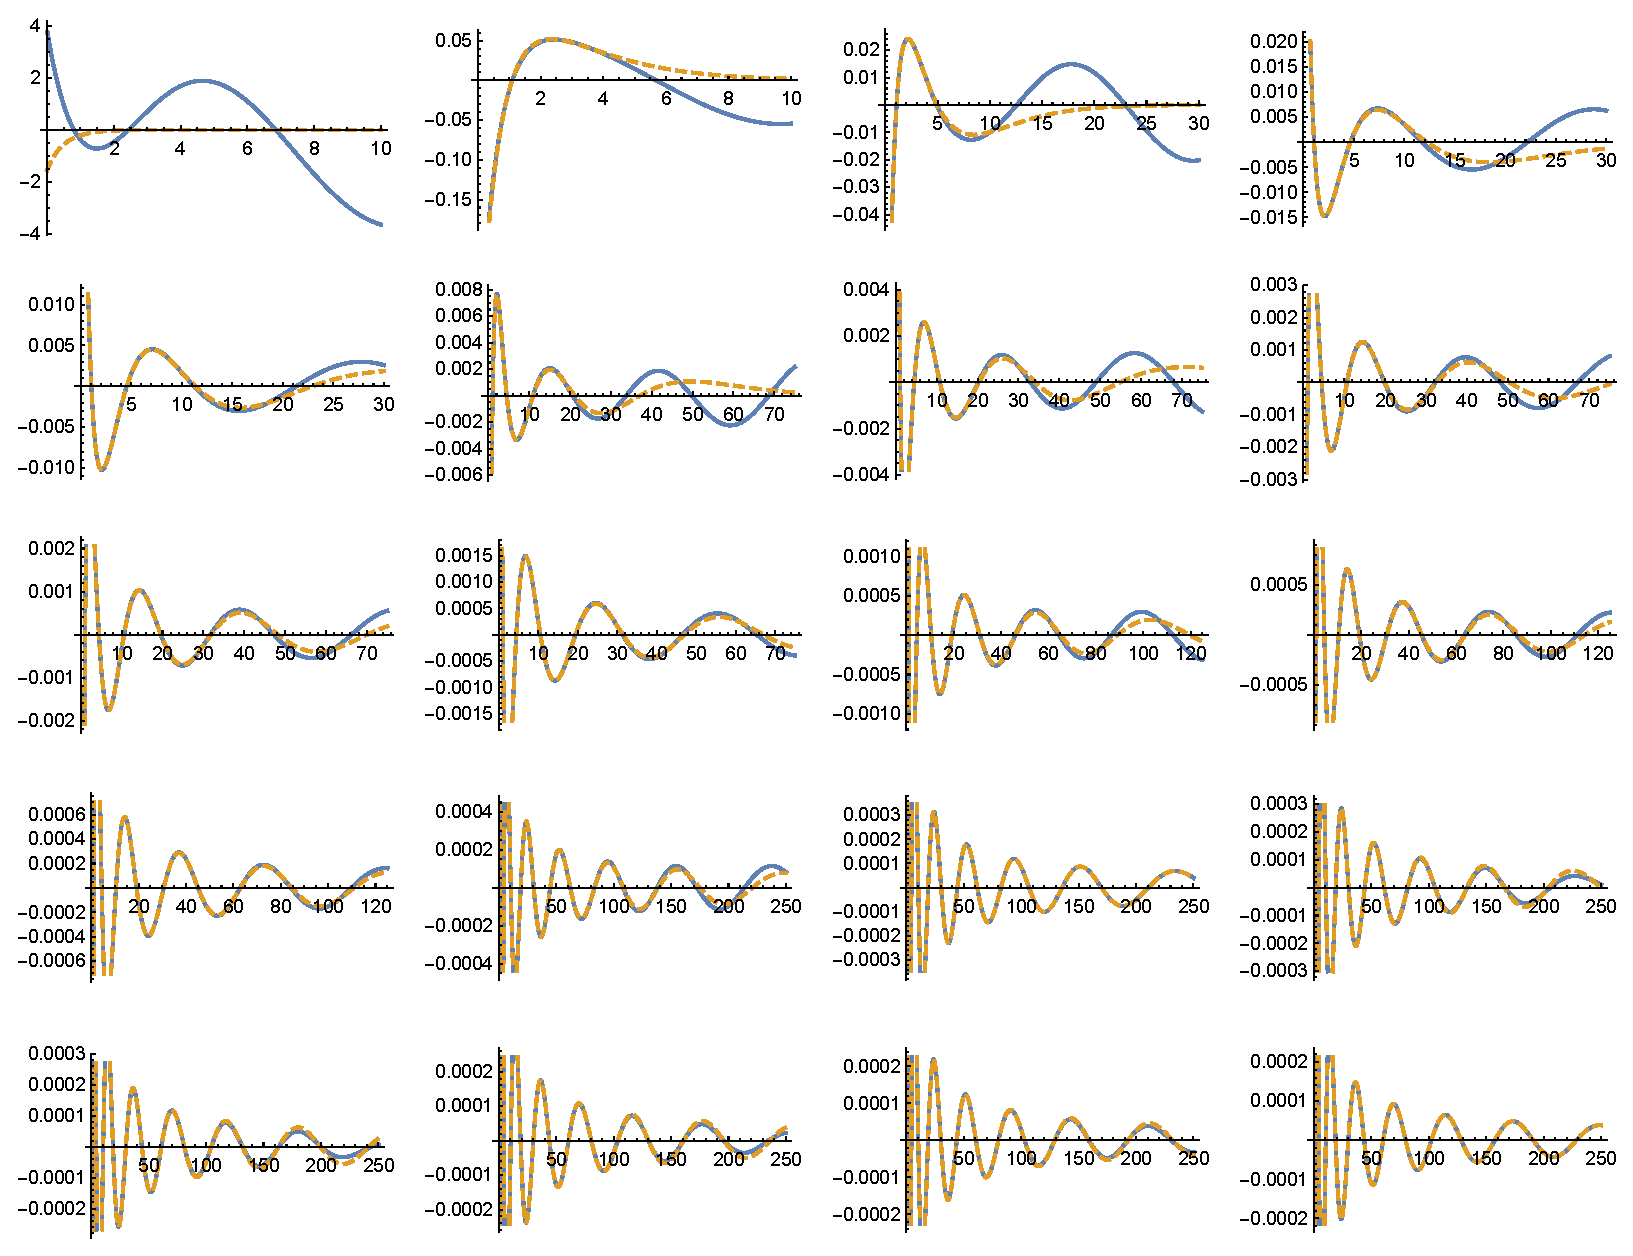
\includegraphics[width=6in]{psir_2.eps}
  \caption{$\psi_{eff}(r)(r>a)$在前20个能级与真实波函数的对比}
\end{figure}
但若再加上$\overline{Z}(r)\psi_{eff}(r)$,则可让$\psi_{true}(r)$在$r>a$时也能成立。

加上$\overline{Z}(r)$,$\psi_{true}(r)$可写为
\begin{equation}\label{psi0ra}
  \psi_{true}(r)=\overline{Z}(r)\psi_{eff}(r)+\overline{\gamma}(r)\int\dd^3r\psi_{eff}\delta^3_a(\vb{r})+\overline{\eta}(r)a^2\int\dd^3r\psi_{eff}\laplacian{\delta^3_a(\vb{r})}+\mathcal{O}(a^3)
\end{equation}
于是可以得到$\psi_{true}(r)$的图像。
\begin{figure}[!htbp]
  \centering
  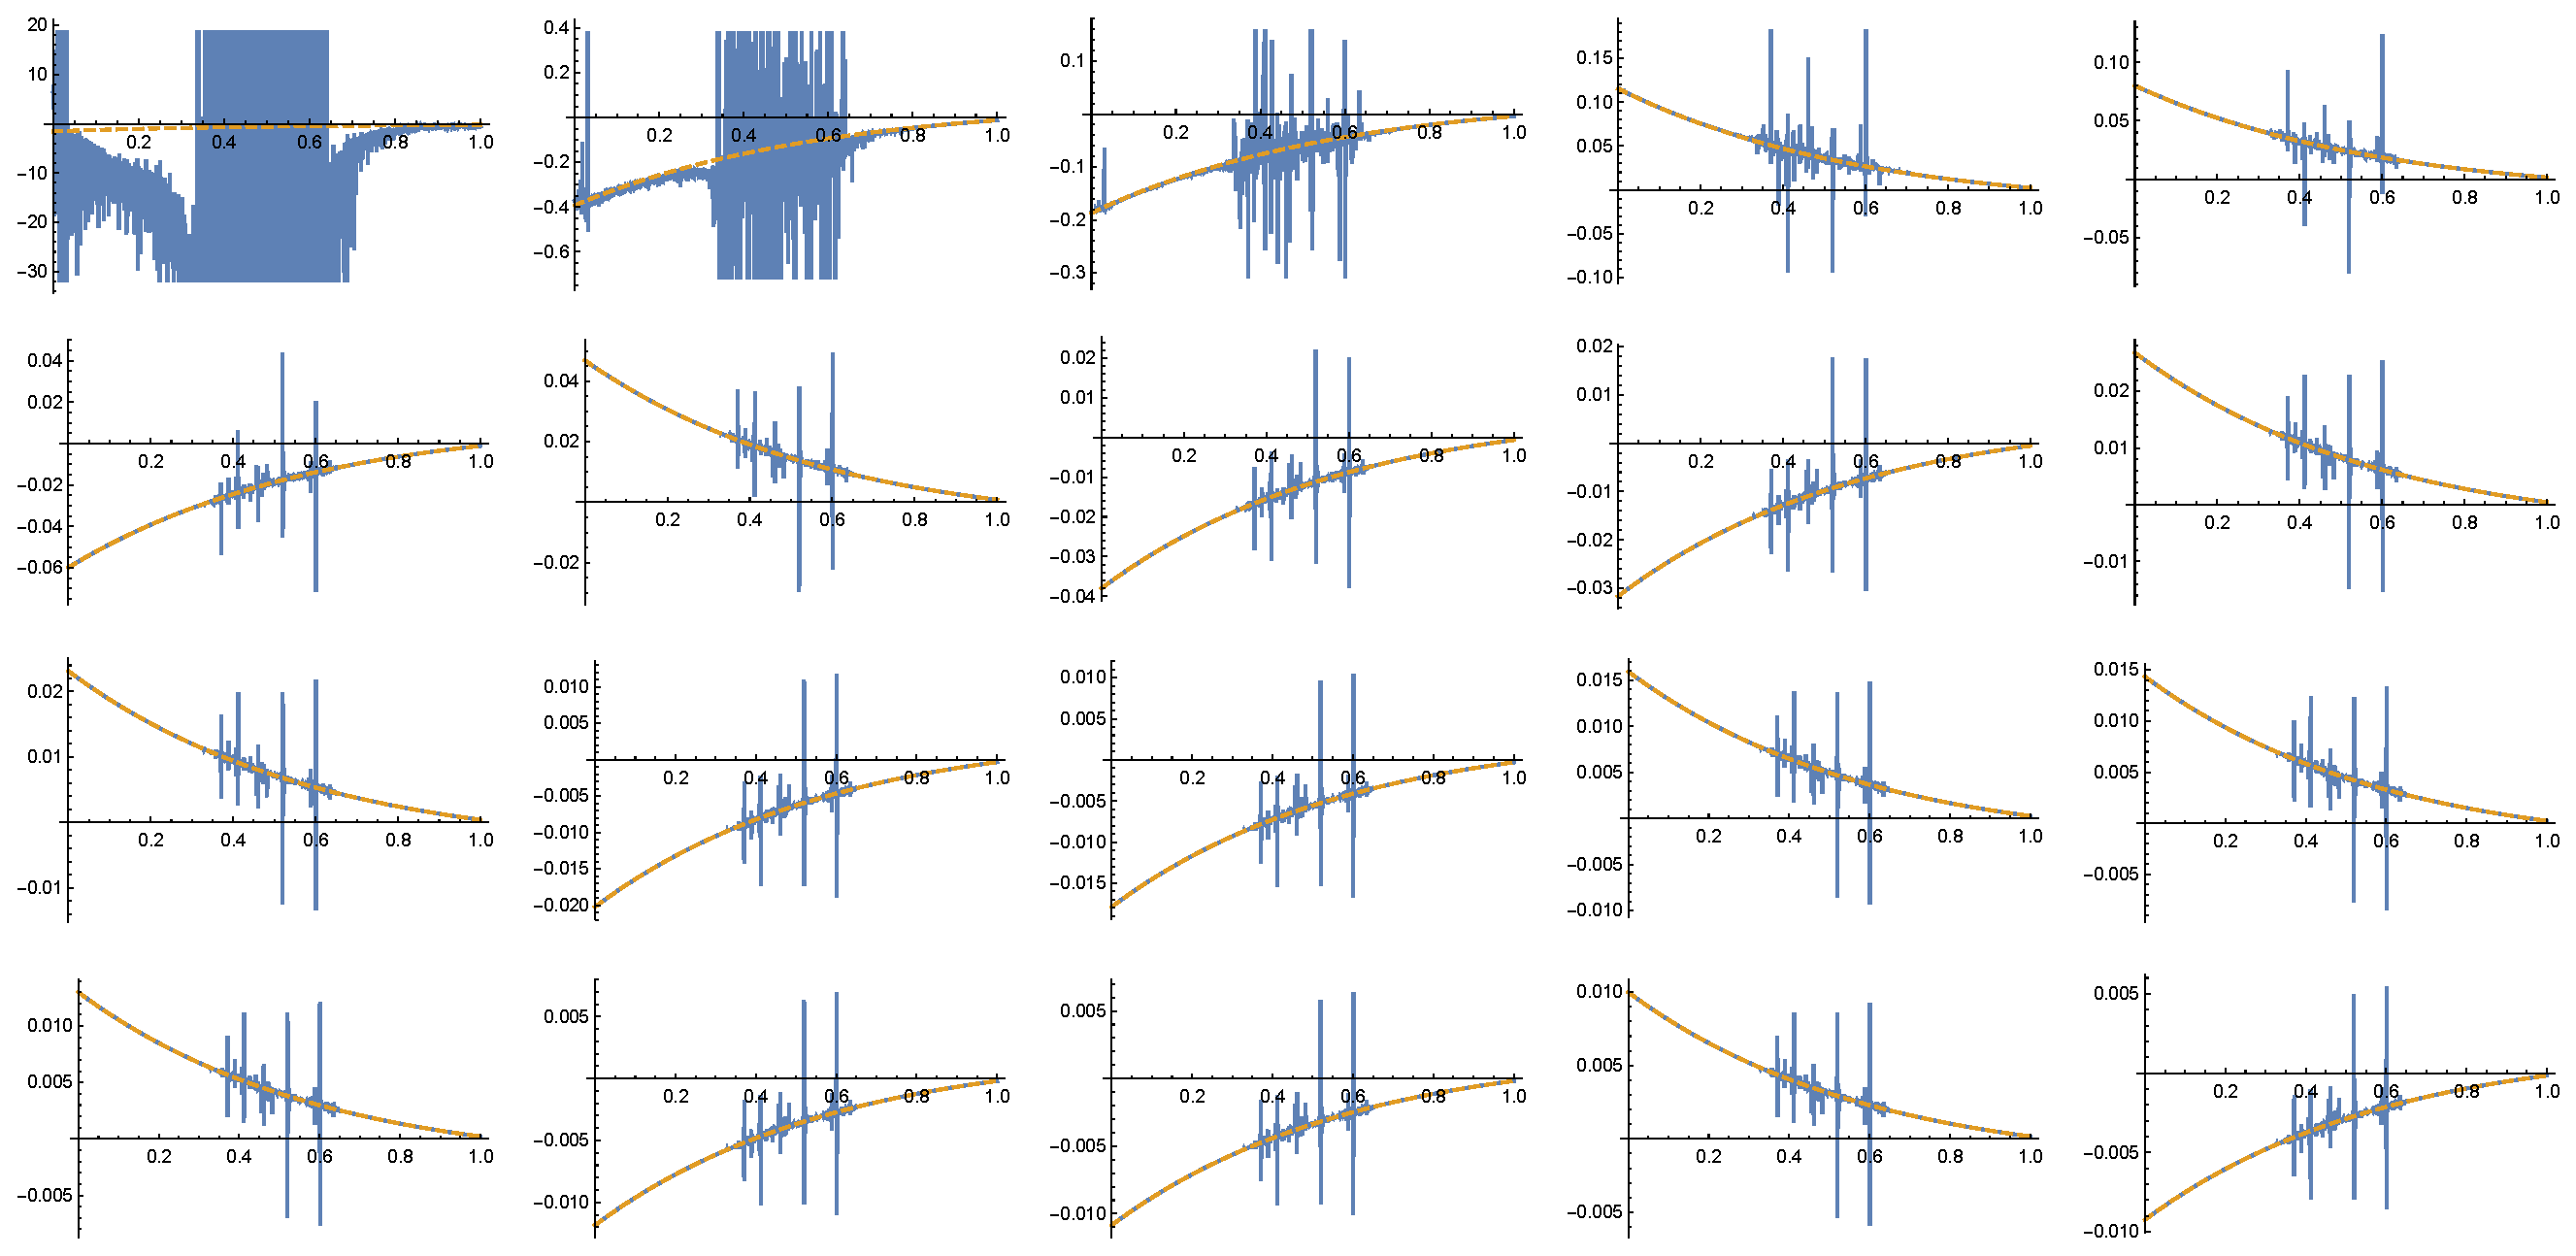
\includegraphics[width=6in]{psirmodified2.eps}
  \caption{$\psi_{eff}(r)(r>a)$在前20个能级与真实波函数的对比}
\end{figure}\\
可以发现,对于几乎所有能级(除了1S外),大范围的$r$内基本都与真实波函数一致。但是图像中的波函数并不是完全光滑的,这是因为\eqref{psi0ra}中的参数不止有一种可能,而不光滑的地方则是参数从一种可能跳到另一种可能所导致的。
\begin{figure}[!htbp]
  \centering
  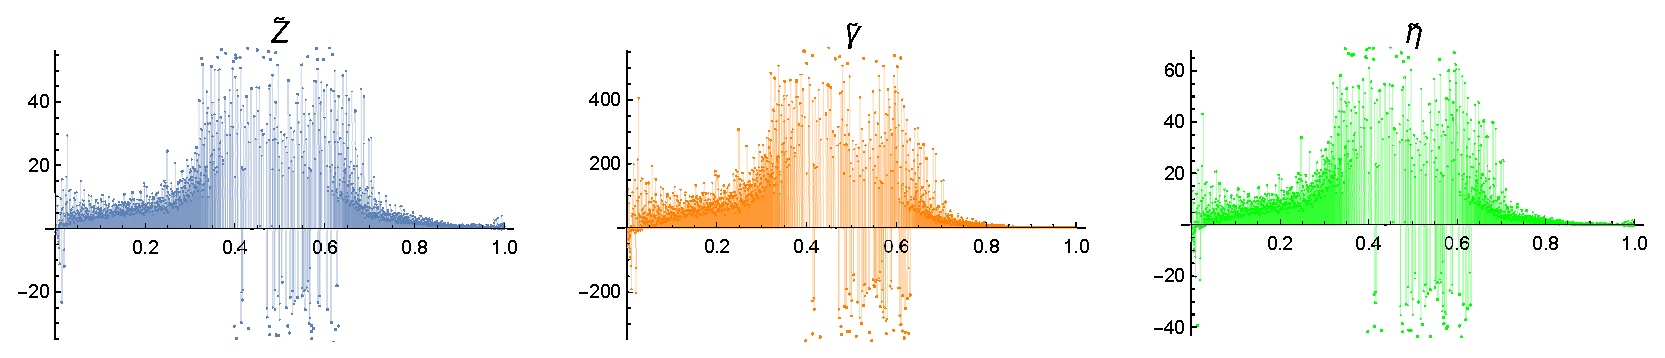
\includegraphics[width=6in]{psirmodified2_2.eps}
  \caption{$\overline{Z}(r)$、$\overline{\gamma}(r)$、$\overline{\eta}(r)$ 的取值}
\end{figure}

$\laplacian{\psi_{true}(r)}$同样可以用相同的办法求出。对方程\eqref{psi0r}左右同时求导后可以得到
\begin{alignat}{1}\label{psi0rl}
  \laplacian{\psi_{true}(r)}=&\overline{\gamma}(r)\int\dd^3r\psi_{eff}\delta^3_a(\vb{r})+\overline{\gamma'}(r)\int\dd^3r\laplacian{\bqty{\psi_{eff}\delta^3_a(\vb{r})}}+\overline{\eta}(r)a^2\int\dd^3r\psi_{eff}\laplacian{\delta^3_a(\vb{r})}
 \nonumber\\&+\overline{\eta'}(r)a^2\int\dd^3r\laplacian{\bqty{\psi_{eff}\laplacian{\delta^3_a(\vb{r})}}}+\mathcal{O}(a^3)
\end{alignat}
其中可以证明$\int\dd^3r\laplacian{\bqty{\psi_{eff}\delta^3_a(\vb{r})}}$与$\int\dd^3r\laplacian{\bqty{\psi_{eff}\laplacian{\delta^3_a(\vb{r})}}}$之值为0。于是\eqref{psi0rl}仅剩两项
\begin{equation}\label{psi0rl2}
  \laplacian{\psi_{true}(r)}=\overline{\gamma}(r)\int\dd^3r\psi_{eff}\delta^3_a(\vb{r})+\overline{\eta}(r)a^2\int\dd^3r\psi_{eff}\laplacian{\delta^3_a(\vb{r})}+\mathcal{O}(a^3)
\end{equation}
其形式与\eqref{psi0r}基本相同。画出$r<a$时的图像,则为
\begin{figure}[!htbp]
  \centering
  \includegraphics[width=6in]{psirlap.eps}
  \caption{$\psi_{eff}(r)(r<a)$在前20个能级与真实波函数的对比}
\end{figure}
\clearpage
\section{有效理论应用于库伦势}
\subsection{确定有效势的具体形式}
对于库伦势加一个短程势的“真实势场”形式,有效理论可以做到较高的精确程度。但是对于纯粹的库伦势,之前的有效理论所得出的结论是否仍然适用呢?

给定一个吸引的库伦势
\begin{equation}
  V(\vb{r})=-\frac{\alpha}{r}
\end{equation}
根据之前的结论,有效势可以定为
\begin{equation}
  V_{eff}(\vb{r})=-\frac{\alpha}{r}\erf(\frac{r}{\sqrt{2}a})+c a^2\delta_a^3(\vb{r})
\end{equation}
在之前的讨论中,库伦势的有效理论中参数$a$并不能像加了一个短程势之后那样找到一个最佳值,为了计算方便,我取$\alpha=0.1$,$m=10$,而$a=0.1$。
如前利用$E=10^{-10}$的相移确定参数$c$的值为$c=-0.692027$,即可得到有效势的具体形式。
\subsection{束缚能与相移}
利用上一节所给出的有效势,可以用非微扰方法计算得出有效理论所给出的S波束缚能与相移如下:
\begin{table}[!htbp]
  \centering
  \begin{tabular}{|cccccc|}
    \hline
    % after \\: \hline or \cline{col1-col2} \cline{col3-col4} ...
    能级 & 束缚能 & 相对误差 & 能级 & 束缚能 & 相对误差 \\
    1S & 0.050079 & 0.000157396 & 11S & 0.000413223 & $1.17148\times10^{-7}$ \\
    2S & 0.0125002 & 0.0000195344 & 12S & 0.000347222 & $9.02323\times10^{-8}$ \\
    3S & 0.00555559 & $5.78045\times10^{-6}$ & 13S & 0.000295858 & $7.09695\times10^{-8}$ \\
    4S & 0.00312501 & $2.43753\times10^{-6}$ & 14S & 0.000255102 & $5.68217\times10^{-8}$ \\
    5S & 0.00200000 & $1.24775\times10^{-6}$ & 15S & 0.000222222 & $4.61979\times10^{-8}$ \\
    6S & 0.00138889 & $7.21997\times10^{-7}$ & 16S & 0.000195313 & $3.08657\times10^{-8}$ \\
    7S & 0.00102041 & $4.54638\times10^{-7}$ & 17S & 0.000173010 & $3.17355\times10^{-8}$ \\
    8S & 0.000781250 & $3.04558\times10^{-7}$ & 18S & 0.000154321 & $2.67346\times10^{-8}$ \\
    9S & 0.000617284 & $2.13895\times10^{-7}$ & 19S & 0.000138504 & $2.27319\times10^{-8}$ \\
    10S & 0.00050000 & $1.55926\times10^{-7}$ & 20S & 0000125000 & $1.94894\times10^{-8}$ \\
    \hline
  \end{tabular}
  \caption{库伦势有效理论S波束缚能}
\end{table}
\clearpage
\begin{table}[!htbp]
  \centering
  \begin{tabular}{|cccccc|}
    \hline
    % after \\: \hline or \cline{col1-col2} \cline{col3-col4} ...
    能量 & 相移 & 相对误差 & 能量 & 相移 & 相对误差 \\
    $10^{-5}$ & -0.214255 & $5.89345\times10^{-9}$ & $0.03$ & 0.536858 & 0.000120999 \\
    $0.001$ & 0.455357 & 0.0000128542 & $0.07$ & 0.386058 & 0.000424473 \\
    $0.003$ & 0.470201 & 0.000111731 & $0.1$ & -0.737847 & 0.000452845 \\
    $0.007$ & 0.244908 & 0.0000459522 & $0.3$ & -1.30762 & 0.000609344 \\
    $0.01$ & -1.05657 & 0.0000237531 & $0.7$ & 0.631691 & 0.00203284 \\
    \hline
  \end{tabular}
  \caption{库伦势有效理论S波相移($r=50$)}
\end{table}
\subsection{$\expval{\vb{p}^4}$矩阵元与$\psi(0)$}
类似于式\eqref{p4true}、\eqref{psi0},$\expval{\vb{p}^4}$矩阵元与$\psi(0)$在有效理论中的修正可由下式给出(由于有效势仅精确到$\mathcal{O}(a^2)$,故抛去$\laplacian{\delta^3_a(\vb{r})}$项):
\begin{eqnarray}
  \expval{\vb{p}^4}_{true}&=&Z\expval{\vb{p^4}}_{eff}+\frac{\gamma}{a}\expval{\delta^3_a(\vb{r})}_{eff}+\mathcal{O}(a)\\
   \psi_{true}(0)&=&\overline{\gamma}\int\dd^3r\psi_{eff}\delta^3_a(\vb{r})+\mathcal{O}(a)
\end{eqnarray}
同样可以给出有效理论中$\expval{\vb{p}^4}$矩阵元与$\psi(0)$的值(库伦势对应的$\expval{\vb{p}^4}$即由解析方法得出)。
\begin{figure}[!htbp]
  \centering
  \includegraphics[width=6in]{Test_Coulomb_7.eps}
  \caption{有效理论束缚能、$\expval{\vb{p}^4}$矩阵元与$\psi(0)$ 相对于库伦势解析解的误差}
\end{figure}
%\begin{table}[!hbtp]
%  \centering
%  \begin{tabular}{|cccccc|}
%    \hline
%    % after \\: \hline or \cline{col1-col2} \cline{col3-col4} ...
%    能级 & $\expval{\vb{p}^4}$ & $\expval{\vb{p^4}}_{eff}$ & $\expval{\vb{p^4}}_{eff}$相对误差 & $\expval{Z\vb{p}^4+\gamma \delta^3_a/a+\dots}_{eff}$ & 修正后相对误差 \\
%    \hline
%    1S & 75.0651 & 6.39016&0.914872 & 86.2584&0.149114 \\
%    2S & 5.89805 & 1.80467&0.694022 & 5.63427&0.0447230 \\
%    3S & 1.38388 & 0.459182&0.668193 & 1.37834&0.00400119 \\
%    4S & 0.533537 & 0.181115&0.660539 & 0.533006&0.000995149 \\
%    5S & 0.259685 & 0.0892336&0.656377 & 0.259594&0.000349898 \\
%    6S & 0.145438 & 0.0503636&0.653711 & 0.145417&0.000142768 \\
%    7S & 0.0895058 & 0.0311615&0.651849 & 0.895003&0.0000608579 \\
%    8S & 0.0589478 & 0.0206038&0.650473 & 0.0589463&0.0000247520 \\
%    9S & 0.0408594 & 0.0143248&0.649413 & 0.0408591&$7.89362\times10^{-6}$ \\
%    10S& 0.0294762 & 0.0103588 & 0.648572 & 0.0294762 & $0.\times10^{-50}$\\
%    11S& 0.0219577 & 0.00773158 & 0.647888 & 0.0219578 & $2.86723\times10^{-6}$\\
%    12S& 0.0167936 & 0.00592277 & 0.647320 & 0.0167937 & $3.65482\times10^{-6}$\\
%    13S& 0.0131299 & 0.00463692 & 0.646842 & 0.0131299 & $3.06033\times10^{-6}$\\
%    14S& 0.0104589 & 0.00369791 & 0.646433 & 0.0104589 & $1.68057\times10^{-6}$\\
%    15S& 0.00846592 & 0.00299626 & 0.646080 & 0.00846592 &  $0.\times10^{-50}$\\
%    16S& 0.00694880 & 0.00246146 & 0.645772 & 0.00694878 & $1.78021\times10^{-6}$\\
%    17S& 0.00577356 & 0.00204673 & 0.645500 & 0.00577354 & $3.67384\times10^{-6}$\\
%    18S& 0.00484908 & 0.00172016 & 0.645260 & 0.00484906 & $5.47461\times10^{-6}$\\
%    19S& 0.00411194 & 0.00145962 & 0.645029 & 0.00411195 & $2.37062\times10^{-6}$\\
%    20S& 0.00503698 & 0.00278627 & 0.446837 & 0.00503698 & $0.\times10^{-50}$\\
%    \hline
%  \end{tabular}
%  \caption{$\expval{\vb{p}^4}$矩阵元在库伦势及其有效理论中的对比}
%\end{table}
%\begin{table}[!htbp]
%  \centering
%  \begin{tabular}{|cccccc|}
%    \hline
%    % after \\: \hline or \cline{col1-col2} \cline{col3-col4} ...
%    能级 & $\psi(0)$ & $\psi_{eff}(0)$ & $\psi_{eff}(0)$ 相对误差& $\overline{\gamma}\int\psi_{eff}\delta^3_a+\dots$ & 修正后相对误差 \\
%    \hline
%    1S & -1.54924 & -0.542484 &0.64984& 4.11644&3.65707 \\
%    2S & -0.392598 & -0.194805 &0.503805& -0.377193&0.0392382 \\
%    3S & -0.187001 & -0.0938498 &0.498132& -0.186328&0.00360212 \\
%    4S & 0.115323 & 0.0578526 &0.498341& 0.115242&0.000698381 \\
%    5S & 0.0801566 & 0.0401962 &0.498529& 0.0801444&0.000151733 \\
%    6S & -0.0598462 & -0.0300043 &0.498643& -0.0598454&0.0000141098 \\
%    \hline
%  \end{tabular}
%  \caption{$\psi(0)$在真实势及有效理论(相移)中的对比}
%\end{table}
\clearpage
\section{有效理论在微扰方法中的应用}
\subsection{确定有效势}
对于哈密顿量
\begin{equation}\label{CoulombSmall}
  H=\frac{\vb{p}^2}{2m}-\frac{\alpha}{r}
\end{equation}
其中$\alpha=0.01$,$m=100$,其有效理论中的哈密顿量为
\begin{equation}\label{CoulombSmall}
  H_{eff}=\frac{\vb{p}^2}{2m}-\frac{\alpha}{r}erf(\frac{r}{\sqrt{2}a})-2\pi\alpha ca^2\delta_a^3(\vb{r})
\end{equation}
$\delta_a^3(\vb{r})$同上。

由解析方法可以轻松导出该势的束缚能,1S到20S为:
\begin{table}[!htbp]
  \centering
  \begin{tabular}{|cccc|}
    \hline
    % after \\: \hline or \cline{col1-col2} \cline{col3-col4} ...
    能级&束缚能&能级&束缚能\\\hline
    1S & 0.005 & 11S & 0.0000413223 \\
    2S & 0.00125 & 12S & 0.0000347222 \\
    3S & 0.000555556 & 13S & 0.0000295858 \\
    4S & 0.0003125 & 14S & 0.0000255102 \\
    5S & 0.0002 & 15S & 0.0000222222 \\
    6S & 0.000138889 & 16S & 0.0000195313 \\
    7S & 0.000102041 & 17S & 0.000017301 \\
    8S & 0.000078125 & 18S & 0.0000154321 \\
    9S & 0.0000617284 & 19S & 0.0000138504 \\
    10S & 0.00005 & 20S & 0.0000125 \\
    \hline
  \end{tabular}
  \caption{$-\displaystyle\frac{\alpha}{r}$束缚能解析解}
\end{table}

通过有效理论,在确定参数$c$的值后可以给出较精确的束缚能。

首先利用一级玻恩近似确定参数$c$的值。对$H$,其一级玻恩近似的散射振幅为(去掉相同的系数$\displaystyle\frac{m}{2\pi\hbar^2}$)
\begin{equation}
  f^{(1)}(\vb{q})=\int\dd^3 x' e^{-i\vb{q}\cdot\vb{x'}}V=-\frac{4\pi\alpha}{q^2}
\end{equation}
其中$\vb{q}=\vb{k_0}-\vb{k'}$为动量转移。而对$H_{eff}$,有
\begin{eqnarray}\label{Heff}
  f_{eff}^{(1)}(\vb{q})&=&-\frac{4\pi\alpha}{q^2}e^{-q^2a^2/2}(1+cq^2a^2/2)\\
  &=&-\frac{4\pi\alpha}{q^2}(1+(c-1)q^2a^2/2+\mathcal{O}(q^4a^4))
\end{eqnarray}
$c=0$时,其1S能级束缚能相对误差为0.0387861\%,而其1S到20S能级相对误差的平均值为0.00697818\%。若令$c=1$,则有效势为
\begin{equation}
  V_{eff}=-\frac{\alpha}{r}erf(\frac{r}{\sqrt{2}a})-2\pi\alpha a^2\delta_a^3(\vb{r})
\end{equation}
在$a=0.01$时,由有效势导出的束缚能及其与解析解的相对误差如下表:
\begin{table}[!htbp]
  \centering
  \begin{tabular}{|cccccc|}
    \hline
    % after \\: \hline or \cline{col1-col2} \cline{col3-col4} ...
    能级&束缚能&相对误差&能级&束缚能&相对误差\\\hline
    1S & 0.00499998 & $3.61412\times10^{-6}$ & 11S & 0.0000413223 & $3.27197\times10^{-7}$\\
    2S & 0.00125 & $1.83241\times10^{-6}$ & 12S & 0.0000347222 & $2.68281\times10^{-7}$\\
    3S & 0.000555556 & $1.77179\times10^{-8}$ & 13S & 0.0000295858 & $2.78941\times10^{-7}$\\
    4S & 0.0003125 & $9.04534\times10^{-7}$ & 14S & 0.0000255102 & $2.57908\times10^{-7}$\\
    5S & 0.0002 & $7.10634\times10^{-7}$ & 15S & 0.0000222222 & $2.30776\times10^{-7}$\\
    6S & 0.000138889 & $5.8436\times10^{-7}$ & 16S & 0.0000195313 & $2.25173\times10^{-7}$\\
    7S & 0.000102041 & $5.13932\times10^{-7}$ & 17S & 0.000017301 & $2.1558\times10^{-7}$\\
    8S & 0.000078125 & $4.49199\times10^{-7}$ & 18S & 0.0000154321 & $2.04102\times10^{-7}$\\
    9S & 0.0000617284 & $3.98123\times10^{-7}$ & 19S & 0.0000138504 & $1.92648\times10^{-7}$\\
    10S & 0.00005 & $3.54257\times10^{-7}$ & 20S & 0.0000125 & $1.85357\times10^{-7}$\\
    \hline
  \end{tabular}
  \caption{一级微扰有效势导出的束缚能及其与解析解的相对误差}
\end{table}

当进一步计算二级玻恩近似的时候,由
\begin{equation}
  T=V+V\frac{1}{E_i-E_m+i\hbar\epsilon}V
\end{equation}
有
\begin{equation}
  V\ket{\psi^{(+)}}=T\ket{\vb{k}}=V\ket{\vb{k}}+V\frac{1}{E_i-E_m+i\hbar\epsilon}V\ket{\vb{k}}
\end{equation}
则
\begin{eqnarray}
% \nonumber % Remove numbering (before each equation)
  f(\vb{k_0},\vb{k'}) &=& (2\pi)^3\mel{\vb{k'}}{V}{\psi^{(+)}}\\
   &=& (2\pi)^3(\mel{\vb{k'}}{V}{\vb{k_0}}+\mel{\vb{k'}}{V\frac{1}{E_i-E_m+i\hbar\epsilon}V}{\vb{k_0}}) \\
   &=& f^{(1)}(\vb{k_0},\vb{k'})+f^{(2)}(\vb{k_0},\vb{k'})
\end{eqnarray}
$f^{(1)}(\vb{k_0},\vb{k'})$如前所示,对于$f^{(2)}(\vb{k_0},\vb{k'})$,可将之化成与$f^{(1)}(\vb{k_0},\vb{k'})$相关的积分形式:
\begin{eqnarray}
  f^{(2)}(\vb{k_0},\vb{k'})&=&(2\pi)^3\mel{\vb{k'}}{V\frac{1}{E_i-E_m+i\hbar\epsilon}V}{\vb{k_0}} \\
  &=&\int\frac{\dd^3k''}{(2\pi)^3}f^{(1)}(\vb{k''},\vb{k'})\frac{1}{E_i-E_m+i\hbar\epsilon}f^{(1)}(\vb{k_0},\vb{k''})\\
  &=&\int\frac{\dd^3k''}{(2\pi)^3}f^{(1)}(\vb{k''},\vb{k'})\frac{2m}{k_0^2-k''^2+2mi\hbar\epsilon}f^{(1)}(\vb{k_0},\vb{k''})
\end{eqnarray}
设$\vb{k}=\vb{k_0}-\vb{k''}$,则$\vb{k}-\vb{q}=\vb{k'}-\vb{k''}$,将$\epsilon$重新定义为$2m\epsilon$,则有
\begin{equation}
  f^{(2)}=\int\frac{\dd^3k}{(2\pi)^3}f^{(1)}(\vb{k}-\vb{q})\frac{2m}{k_0^2-(\vb{k}-\vb{k_0})^2+i\hbar\epsilon}f^{(1)}(\vb{k})
\end{equation}
对于一阶玻恩近似而言,由之前给定的$c$,库伦势与有效势的散射振幅几乎完全相同,仅相差$\mathcal{O}(k^4a^4)$。二阶情况下两势散射振幅之差则主要由$f^{(2)}$与$f_{eff}^{(2)}$贡献,且相对于$k$,$p$、$q$可以被忽略:
\begin{eqnarray}
% \nonumber % Remove numbering (before each equation)
  f_{eff}^{(2)}-f^{(2)} &=& \int\frac{\dd^3k}{(2\pi)^3}\bqty{\pqty{\frac{-4\pi\alpha}{k^2}\frac{-2m}{k^2}\frac{-4\pi\alpha}{k^2}}e^{-k^2a^2}(1+k^2a^2/2)^2-\pqty{\frac{-4\pi\alpha}{k^2}\frac{-2m}{k^2}\frac{-4\pi\alpha}{k^2}}} \\
   &=& \frac{10}{3} \sqrt{\pi } \alpha^2  a^3 m
\end{eqnarray}
于是对$c$作修正,令$f_{eff}^{(1)}(\vb{q})$的第二项
\begin{equation}
  -\frac{4\pi\alpha}{q^2}(c-1)q^2a^2/2=-\frac{10}{3} \sqrt{\pi } \alpha^2  a^3 m
\end{equation}
最终得到$\displaystyle c=1+\frac{5}{3\sqrt{\pi}}\alpha a m=1.00940316$。
\begin{table}[!htbp]
  \centering
  \begin{tabular}{|cccccc|}
    \hline
    % after \\: \hline or \cline{col1-col2} \cline{col3-col4} ...
    能级&束缚能&相对误差&能级&束缚能&相对误差\\\hline
    1S & 0.005 & $2.12769\times10^{-8}$ & 11S & 0.0000413223 & $4.18928\times10^{-9}$\\
    2S & 0.00125 & $1.33472\times10^{-8}$ & 12S & 0.0000347222 & $4.21076\times10^{-9}$\\
    3S & 0.000555556 & $2.5859\times10^{-9}$ & 13S & 0.0000295858 & $2.66263\times10^{-10}$\\
    4S & 0.0003125 & $3.1513\times10^{-8}$ & 14S & 0.0000255102 & $8.8104\times10^{-12}$\\
    5S & 0.0002 & $1.04359\times10^{-9}$ & 15S & 0.0000222222 & $2.89155\times10^{-10}$\\
    6S & 0.000138889 & $9.14987\times10^{-9}$ & 16S & 0.0000195313 & $2.68476\times10^{-9}$\\
    7S & 0.000102041 & $1.30144\times10^{-8}$ & 17S & 0.000017301 & $2.15443\times10^{-9}$\\
    8S & 0.000078125 & $6.59177\times10^{-9}$ & 18S & 0.0000154321 & $2.08666\times10^{-9}$\\
    9S & 0.0000617284 & $7.4271\times10^{-9}$ & 19S & 0.0000138504 & $2.99971\times10^{-9}$\\
    10S & 0.00005 & $5.1792\times10^{-9}$ & 20S & 0.0000125 & $2.81353\times10^{-9}$\\
    \hline
  \end{tabular}
  \caption{二级微扰有效势导出的束缚能及其与解析解的相对误差}
\end{table}

应用之前所给出的有效势\eqref{Heff},参数$c$同样可以利用非微扰方法计算出来。类似之前的讨论,利用$E=10^{-10}$处相移确定$c$的值,得到$c=1.0094723$。其束缚能结果与上类似。
%\subsection{$\expval{\vb{p}^4}$矩阵元}
\clearpage
%\section{相对论修正}
%对于
%\clearpage
\section{不同短程势}
将库伦势所附加的短程势替换为5种完全不同的短程势,所得到的模型仅在低能量处具有极相似的特征,较高能量的行为则完全不同,势的形式如下:
\begin{eqnarray}
% \nonumber % Remove numbering (before each equation)
V_1&=&-\frac{\alpha}{r}+\begin{cases}
                          a, & \mbox{if } 0<=r<1 \\
                          0, & \mbox{otherwise}.
                        \end{cases}\\
V_2&=&-\frac{\alpha}{r}+c \frac{e^{-dr}}{r}\\
V_3&=&-\frac{\alpha}{r}+e \frac{e^{-fr^2}}{r}\\
V_4&=&-\frac{\alpha}{r}+g e^{-hr}\\
V_5&=&-\frac{\alpha}{r}+ie^{-jr^2}
\end{eqnarray}
其中参数的具体值不一一列出,图像如下图。
\begin{figure}[!htbp]
  \centering
  \includegraphics[width=6in]{MultiplePotential.eps}
  \caption{不同势函数图像对比}
\end{figure}

从下图可以看出,这些势在低能量处束缚能与相移都极其接近,能量较高处则开始出现差别,$\abs{E}>1$时这一差别就较为明显了。
\begin{figure}[!htbp]
  \centering
  \includegraphics[width=6in]{MultiplePotential_1.eps}
  \caption{不同势束缚能对比}
\end{figure}
\begin{figure}[!htbp]
  \centering
  \includegraphics[width=6in]{MultiplePotential_2.eps}
  \caption{不同势相移对比}
\end{figure}
\clearpage
而采用有效理论之后,其束缚能的结果如下:
\begin{figure}[!htbp]
  \centering
  \includegraphics[width=6in]{MultiplePotential_3.eps}
  \caption{$V_{eff}^{(a^2)}$束缚能误差对比}
\end{figure}
\begin{figure}[!htbp]
  \centering
  \includegraphics[width=6in]{MultiplePotential_5.eps}
  \caption{$V_{eff}^{(a^4)}$束缚能误差对比}
\end{figure}
\clearpage
其相移结果如下:
\begin{figure}[!htbp]
  \centering
  \includegraphics[width=6in]{MultiplePotential_4.eps}
  \caption{$V_{eff}^{(a^2)}$相移误差对比}
\end{figure}
\begin{figure}[!htbp]
  \centering
  \includegraphics[width=6in]{MultiplePotential_6.eps}
  \caption{$V_{eff}^{(a^4)}$相移误差对比}
\end{figure}
\clearpage
$\expval{\vb{p}^4}$矩阵元之值与其在$V_{eff}^{(a^4)}$有效理论中的误差分别如下:
\begin{figure}[!htbp]
  \centering
  \includegraphics[width=6in]{MultiplePotential_7.eps}
  \caption{$\expval{\vb{p}^4}$矩阵元之值}
\end{figure}
\begin{figure}[!htbp]
  \centering
  \includegraphics[width=6in]{MultiplePotential_8.eps}
  \caption{$\expval{\vb{p}^4}$矩阵元在$V_{eff}^{(a^4)}$中的误差}
\end{figure}
\clearpage
$\psi(0)$之值与其在$V_{eff}^{(a^4)}$有效理论中的误差分别如下:
\begin{figure}[!htbp]
  \centering
  \includegraphics[width=6in]{MultiplePotential_7.eps}
  \caption{$\psi(0)$之值}
\end{figure}
\begin{figure}[!htbp]
  \centering
  \includegraphics[width=6in]{MultiplePotential_8.eps}
  \caption{$\psi(0)$在$V_{eff}^{(a^4)}$中的误差}
\end{figure}
\clearpage
\begin{thebibliography}{b}

\bibitem{Lepage}
Lepage P. How to Renormalize the Schrodinger Equation[J]. Nuclear Theory, 1997.
\bibitem{sakurai}
Sakurai J J, Tuan S F, Commins E D. Modern Quantum Mechanics, Second Edition. Pearson Schweiz Ag, 2013.
\bibitem{Jinyan}
曾谨言. 量子力学(卷I)(第5版)(现代物理学丛书)(精)[M]. 科学, 2013.
\bibitem{Griffiths}
Griffiths, David Jeffery. Introduction to quantum mechanics. Pearson Education India, 2013.
\bibitem{Chen}
陈鄂生. 量子力学基础教程(第5版)[M]. 山东大学出版社, 2013.
\bibitem{Korsch}
Korsch H J, Glck M. Computing quantum eigenvalues made easy[J]. European Journal of Physics, 2002, 23(23):413-426.
\bibitem{Landau}
朗道, 栗弗席兹. 量子力学:非相对论理论[M]. 高等教育出版社, 2008.
\bibitem{Weinberg}
Weinberg S. Lectures on Quantum Mechanics[J]. Lectures on Quantum Mechanics by Steven Weinberg Cambridge Uk Cambridge University Press, 2012, 83(9):xiv,528.
\bibitem{MMA}
徐安农. 科学计算引论: 基于 Mathematica 的数值分析[M]. 机械工业出版社, 2010.
\bibitem{dong1}
董键. Mathematica与大学物理计算 第2版[M]. 清华大学出版社, 2013.
\end{thebibliography}
\end{document} 